\documentclass[nobib,notoc]{tufte-book}

\hypersetup{colorlinks}% uncomment this line if you prefer colored hyperlinks (e.g., for onscreen viewing)

%%
% Book metadata
\title{A Tufte-Style Book\thanks{Thanks to Edward R.~Tufte for his inspiration.}}
\author[The Tufte-LaTeX Developers]{The Tufte-LaTeX\ Developers}
\publisher{Publisher of This Book}

\input{config-tufte}
% packages
\usepackage[utf8]{inputenc}
\usepackage{libertine}
\usepackage{libertinust1math}
\usepackage[T1]{fontenc}
\usepackage[square,numbers]{natbib}
\bibliographystyle{abbrvnat}

\setlength{\textfloatsep}{5pt}
\setfloatalignment{t}

\date{May 4, 2020}

\setcounter{secnumdepth}{2}

% dotted toc
\usepackage[titles]{tocloft}
\makeatletter
\renewcommand*\l@figure{\@dottedtocline{1}{1.5em}{2.3em}}
\makeatother

% ****************************************************************************************************
% 2. Personal data and user ad-hoc commands (insert your own data here)
% ****************************************************************************************************
\newcommand{\myTitle}{Perceptual Optimizations for Video Capture, Processing, and Storage Systems\xspace}
\newcommand{\mySubtitle}{A dissertation \\
submitted in partial fulfillment of the \\
requirements for the degree of\xspace}
\newcommand{\myDegree}{Doctor of Philosophy\xspace}
\newcommand{\myName}{Amrita Mazumdar\xspace}
\newcommand{\myChair}{Luis Ceze\xspace}
\newcommand{\myOtherChair}{Mark Oskin\xspace}
\newcommand{\myFaculty}{Magda Balazinska\xspace}
\newcommand{\myGSR}{Rebecca Cummings (Art)\xspace}
\newcommand{\myDepartment}{Paul G. Allen School of Computer Science \& Engineering\xspace}
\newcommand{\myUni}{University of Washington\xspace}
\newcommand{\myLocation}{Seattle, WA\xspace}
\newcommand{\myTime}{2020\xspace}
\newcommand{\myVersion}{\classicthesis}



% todo %%%%%%%%%%%%%%%%%%%%%%%%%%%%%%%%%%%%%%%%%%%%%%%%%%%%%%%%%%%%%%%%%%%%%%%%%
\newcommand{\todo}[1]{{\color{red}TODO:#1}}
\newcommand{\tocite}[1]{{\color{blue}\textbf{[[#1]]}}}


% other ones
\newcommand{\name}{Vignette\xspace}
\newcommand{\nameStore}{Vignette Storage\xspace}
\newcommand{\nameCompress}{Vignette Compression\xspace}
\newcommand{\nameArch}{TVA\xspace}
\newcommand{\nameArchprof}{TVAprof\xspace}

\newcommand{\redout}[1]{\textcolor{red}{ #1}}
\newcommand{\blueout}[1]{\textcolor{blue}{ #1}}
\newcommand{\bluecomment}[1]{\textcolor{blue}{ \{$\leftarrow$ #1\}}}

% text expansion macros %%%%%%%%%%%%%%%%%%%%%%%%%%%%%%%%%%%%%%%%%%%%%%%%%%%%%%%%
\newcommand{\etal}{et al.}

% video-related
\newcommand{\avc}{\textsc{h.264}\xspace}
\newcommand{\hevc}{\textsc{hevc}\xspace}
\newcommand{\vpeight}{\textsc{vp8}\xspace}
\newcommand{\vpnine}{\textsc{vp9}\xspace}
\newcommand{\avone}{\textsc{av1}\xspace}
\newcommand{\threesixty}{360$\degree$\xspace}
\newcommand{\lightdb}{LightDB\xspace}

% C++
\newcommand\CC{C\nolinebreak[4]\hspace{-.05em}\raisebox{.4ex}{\relsize{-3}{\textbf{++}}}\xspace}

%%%%%%%%%%%%%%%%%%%%%%%
% NSP packages
%%%%%%%%%%%%%%%%%%%%%%%%%

% fonts & text %%%%%%%%%%%%%%%%%%%%%%%%%%%%%%%%%%%%%%%%%%%%%%%%%%%%%%%%%%%%%%%%%
\usepackage{inconsolata}              % inconsolata for fixed-width
\usepackage{textcomp}              % symbols

% figures %%%%%%%%%%%%%%%%%%%%%%%%%%%%%%%%%%%%%%%%%%%%%%%%%%%%%%%%%%%%%%%%%%%%%%
\usepackage{graphicx}              % includegraphics

% tables %%%%%%%%%%%%%%%%%%%%%%%%%%%%%%%%%%%%%%%%%%%%%%%%%%%%%%%%%%%%%%%%%%%%%%%
\usepackage{booktabs}              % pretty table spacing

% spacing %%%%%%%%%%%%%%%%%%%%%%%%%%%%%%%%%%%%%%%%%%%%%%%%%%%%%%%%%%%%%%%%%%%%%%
\usepackage{relsize}               % \relsize{-1} for macros
\usepackage[export]{adjustbox}

% colors %%%%%%%%%%%%%%%%%%%%%%%%%%%%%%%%%%%%%%%%%%%%%%%%%%%%%%%%%%%%%%%%%%%%%%%
% \usepackage[dvipsnames,table]{xcolor}      % colors, with svg names available
\definecolor{bluekeywords}{rgb}{0.13,0.13,1}
\definecolor{greencomments}{rgb}{0,0.5,0}
\definecolor{redstrings}{rgb}{0.9,0,0}
\definecolor{CTsemi}{gray}{0.55} % chapter numbers will be semi transparent .5 .55 .6 .0
\definecolor{CTcitation}{rgb}{0,0.5,0} % WebGreen
\definecolor{CTurl}{named}{Maroon} % Maroon
\definecolor{CTtitle}{named}{Maroon} % Maroon {cmyk}{0, 0.87, 0.68, 0.32}
\definecolor{CTlink}{named}{RoyalBlue} % RoyalBlue {cmyk}{1, 0.50, 0, 0}
\definecolor{halfgray}{gray}{0.55} % chapter numbers will be semi transparent .5 .55 .6 .0
\definecolor{webgreen}{rgb}{0,0.5,0}
\definecolor{webbrown}{rgb}{0.6,0,0}



% math %%%%%%%%%%%%%%%%%%%%%%%%%%%%%%%%%%%%%%%%%%%%%%%%%%%%%%%%%%%%%%%%%%%%%%%%%
\usepackage{amsmath}
\usepackage{amsfonts}              % provides \mathbb and other stuff
\usepackage{amssymb}               % lots of symbols

% listings %%%%%%%%%%%%%%%%%%%%%%%%%%%%%%%%%%%%%%%%%%%%%%%%%%%%%%%%%%%%%%%%%%%%%
\usepackage{listings}              % code listings
\lstset{language=Python,
  showspaces=false,
  showtabs=false,
  breaklines=true,
  showstringspaces=false,
  breakatwhitespace=true,
  escapeinside={(*@}{@*)},
  commentstyle=\color{greencomments},
  keywordstyle=\color{bluekeywords},
  stringstyle=\color{redstrings},
  basicstyle=\ttfamily
}

% *** SUBFIGURE PACKAGES ***


\newcommand{\MITCMU}{MIT-CMU\xspace}
\newcommand{\ATTFACES}{AT\&T Face Database\xspace}
\newcommand{\LFW}{Labeled Faces in the Wild\xspace}
\newcommand{\ANNA}{ANN accelerator\xspace}
\newcommand{\fscore}{F\textsubscript{1} score\xspace}

\newcommand{\nearsensor}{in-camera\xspace}
\newcommand{\Nearsensor}{In-camera\xspace}
\newcommand{\NearSensor}{In-Camera\xspace}
\newcommand{\NSP}{ICP\xspace}

\newcommand{\farsensor}{off-loaded\xspace}
\newcommand{\Farsensor}{Off-loaded\xspace}
\newcommand{\FarSensor}{Off-Loaded\xspace}
\hyphenation{FPGA reduce FPGAs camera off-load-ing authenti-cation reduct-ion follow-ing comm-unication}


%%%%%%%%%%%
% HFBS macros / packages
%%%%%%%%%%%%%%%%%%%%%%%%
\def\lf{\left\lfloor}
\def\rf{\right\rfloor}
\def\lc{\left\lceil}
\def\rc{\right\rceil}
\usepackage{mathtools}

\usepackage{multirow}
\usepackage{hyphenat}

\DeclarePairedDelimiter{\abs}{\lvert}{\rvert}
\DeclarePairedDelimiter{\norm}{\lVert}{\rVert}
% math %%%%%%%%%%%%%%%%%%%%%%%%%%%%%%%%%%%%%%%%%%%%%%%%%%%%%%%%%%%%%%%%%%%%%%%%%
\usepackage{amsmath}
\usepackage{amsfonts}              % provides \mathbb and other stuff
\usepackage{amssymb}               % lots of symbols
\usepackage{tabularx}
\usepackage{comment}


% graphics %%%%%%%%%%%%%%%%%%%%%%%%%%%%%%%%%%%%%%%%%%%%%%%%%%%%%%%%%%%%%%%%%%%%%%%%%
\usepackage{graphicx}
\graphicspath{{./fig/},{./plots/},{./gfx/},{./hfbs-figs/},{./nsp-figs/},{./vignette-figs/},{./graphics/}}
\setkeys{Gin}{width=\linewidth,totalheight=\textheight,keepaspectratio}

\DeclareGraphicsExtensions{.pdf,.jpeg,.jpg,.png}

\usepackage{algorithm,algpseudocode}
\makeatletter
\def\algbackskip{\hskip\dimexpr-\algorithmicindent+\labelsep}
\def\LState{\State \algbackskip}%
\makeatother

\usepackage{array}
\newcolumntype{C}[1]{>{\centering\let\newline\\\arraybackslash\hspace{0pt}}m{#1}}
\usepackage[normalem]{ulem}

\usepackage{subfig}


% colors %%%%%%%%%%%%%%%%%%%%%%%%%%%%%%%%%%%%%%%%%%%%%%%%%%%%%%%%%%%%%%%%%%%%%%%

\usepackage{colortbl}


\lstdefinestyle{VRQL}{
    language=C++,
    basicstyle=\scriptsize\ttfamily,
    mathescape=true,
    xleftmargin=0.25cm,
    columns=fullflexible,
    morekeywords={Union,Decode,Scan,Select,Map,Partition,Encode,Subquery,Interpolate,Translate,Rotate,Discretize,Store,Update,Create,CreateIndex,DropIndex}
 }


% Generates the index
\usepackage{makeidx}
\makeindex

\begin{document}

% Front matter
\frontmatter

% p1 title
%*******************************************************
% Titlepage
%*******************************************************
\begin{titlepage}
  \begin{fullwidth}
    %\pdfbookmark[1]{\myTitle}{titlepage}
    % if you want the titlepage to be centered, uncomment and fine-tune the line below (KOMA classes environment)
    % \begin{addmargin}[-1cm]{-3cm}
    \begin{center}
        \large

        \hfill

        \vfill

        \begingroup
            \color{CTtitle}\allcaps{\myTitle} \\ \bigskip
        \endgroup

        \smallcaps{\myName} \\ \bigskip \bigskip \bigskip \bigskip
        \bigskip \bigskip

        \mySubtitle \\ \medskip
        \myDegree \\ \medskip
        \myUni \\
        \myTime \\  \bigskip \bigskip \bigskip \bigskip
        \bigskip \bigskip

        Reading Committee: \\ \medskip
        \myChair \\ \medskip
        \myOtherChair \\ \medskip
        \myFaculty \\ \bigskip \bigskip \bigskip \bigskip
        \bigskip \bigskip

        Program Authorized to Offer Degree: \\ \medskip
        \myDepartment \\

        \vfill

    \end{center}
  \end{fullwidth}
\end{titlepage}


% p2 copyright page
\thispagestyle{empty}

\bigskip \bigskip
\textcopyright\ Copyright \myTime \\ \medskip
\myName \\



%\bigskip
%
%\noindent\spacedlowsmallcaps{Supervisors}: \\
%\myProf \\
%\myOtherProf \\
%\mySupervisor
%
%\medskip
%
%\noindent\spacedlowsmallcaps{Location}: \\
%\myLocation
%
%\medskip
%
%\noindent\spacedlowsmallcaps{Time Frame}: \\
%\myTime


% p3 abstract
%*******************************************************
% Abstract
%*******************************************************
%\renewcommand{\abstractname}{Abstract}
\pdfbookmark[1]{Abstract}{Abstract}
% \addcontentsline{toc}{chapter}{\tocEntry{Abstract}}
\begingroup
\let\clearpage\relax
\let\cleardoublepage\relax
\let\cleardoublepage\relax

\thispagestyle{empty}
\begin{center}
    \spacedlowsmallcaps{Abstract} \\
    \bigskip
    {\color{CTtitle}\spacedallcaps{\myTitle} \\ \bigskip
    }
    \bigskip
    \myName \\
    \bigskip
    Chairs of the Supervisory Committee: \\
    Professor \myChair \\
    Associate Professor \myOtherChair \\
    \myDepartment \\
    \bigskip
\end{center}


Visual media is the dominant form of content used in modern computing systems.
Advances in machine learning, virtual reality, and display form factors drive demand for richer visual experiences, putting pressure on systems to efficiently use compute and storage infrastructure.
At the same time, the rapid pace of performance and energy efficiency gains computer architects depended on to meet growing application requirements has slowed.
Designing computer systems to meet the requirements of modern video-based applications requires specialization in compute design, using hardware-software codesign techniques to closely optimize computer system performance for specific visual computing workloads.

This thesis uses perceptual information to optimize the design of video capture, processing and storage systems.
I describe system optimizations using three classes of perceptual cues: structure (e.g., color, depth); semantics (e.g., faces, objects); and saliency (e.g., human visual saliency, neural network feature saliency).
This thesis demonstrates how perceptual information can be used in hardware accelerator designs on ASICs and FPGAs, and in cloud video storage infrastructure.

\endgroup

\vfill


% p4 blank page
\blankpage

% p5 epigraph
%*******************************************************
% Dedication
%*******************************************************

\newpage\thispagestyle{empty}

\noindent \textit{To my parents.}


\bigskip
\bigskip
\bigskip

\noindent A new sense of the notion of information has been constructed around the photographic image.
The photograph is a thin slice of space as well as time.
In a world ruled by photographic images, all borders (``framing'') seem arbitrary\ldots
    %Anything can be separated, can be made discontinuous, from anything else: all that is necessary is to frame the subject differently. (Conversely, anything can be made adjacent to anything else.) Photography reinforces a nominalist view of social reality as consisting of small units of an apparently infinite number--as the number of photographs that could be taken of anything is unlimited. Through photographs, the world becomes a series of unrelated, freestanding particles; and history, past and present, a set of anecdotes and faits divers...  \\
    %The camera makes reality atomic, manageable, and opaque. It is a view of the world which denies interconnectedness, continuity, but which confers on each moment the character of a mystery. Any photograph has multiple meanings; indeed, to see something in the form of a photograph is to encounter a potential object of fascination.
The ultimate wisdom of the photographic image is to say:
    \begin{quote}
      ``There is the surface. Now think--or rather feel, intuit--what is beyond it, what the reality must be like if it looks this way.''
      \end{quote}
\noindent  --- Susan Sontag, \emph{On Photography}


\vfill%
% \begin{center}
%     To my parents. \\
% \end{center}


% p7 blank page
\blankpage

% p8 acks
%*******************************************************
% Acknowledgments
%*******************************************************
\pdfbookmark[1]{Acknowledgments}{acknowledgments}

\bigskip

\begingroup
\let\clearpage\relax
\let\cleardoublepage\relax
\let\cleardoublepage\relax
\chapter*{Acknowledgments}

\setlength{\parskip}{5pt}%
\setlength{\parindent}{0pt}%

Completing a PhD is a singular achievement but also one impossible to achieve alone.

I must first thank my co-advisors, Luis Ceze and Mark Oskin.
To be coadvised is to be paired with two indefatigable champions with no clear model for consensus.
Luis taught me to be ambitious in research impact and aggressive with my creativity.
Mark taught me to be discriminating in idea selection and lighthearted in my daily work.
The act of balancing their unending ideas and criticism has shaped the mold of my research forever.
Thank you for advising me!

Like any PhD student at the Allen School for Computer Science, I had not only two advisors but also a cabal of faculty and industry researchers helping me along.
Notably, Magda Balazinska taught me how to lift architecture research into the world of systems and how to lead research collaborations with thoughtfulness and clarity.
Other mentors improved my work through significant revision, feedback, entropy, and expertise: Jon Barron, Alvin Cheung, David Gallup, Warren Hunt, Anton Kaplanyan, Visvesh Sathe, Steve Seitz.

Much as I tried to conduct a research project without anyone's help, I could not have completed a single page of this dissertation without my friends and lab mates: Armin Alaghi, Meghan Cowan, Maureen Daum, Emily Furst, Brandon Haynes, Brandon Holt, Sung Kim, Vincent Lee, Ming Liu, Liang Luo, Thierry Moreau, Brandon Myers, Jacob Nelson, Benjamin Ransford, Adrian Sampson, Pratyush Patel, Luis Vega, Mark Wyse, Eddie Yan. Very special thanks to my friends Kira Goldner, Ellie Levey, Lucy Lin, and Maarten Sap for providing company at a fortifying brunch as necessary.

Preparing a dissertation may be hard, but running the operations that allow research to be researched and innovation to be innovated is much harder. None of my work could be possible without the emotional and infrastructural support of Elise Dorough, Melody Kadenko, Amanda Robles, and Anna Wehovsky.

My arrival at the University of Washington would not have occurred without a cosmic alignment of advising from faculty at Columbia University: Steven Edwards, Martha Kim, and Shree Nayar. The CRA-W's DREU program connected me to Iris Bahar at Brown University, my first guide through computer engineering.

I am grateful to the staff of High Technology High School for introducing me to research, and Gary S. Settles for being my first faculty mentor. My original education on abstraction and interfaces came from a decade of piano lessons from Beth S. Chen.

Finally, thank you to my parents, Rekha Datta and Subrata Mazumdar, for supporting me in a great many things but especially this process.

No level of thanks could possibly be sufficient to account for Gregory T. Woolston's contribution to this work; I will not even begin to try.

\endgroup


% p9 blank page
\blankpage


% p10 contents
\tableofcontents

\cleardoublepage

% Start the main matter (normal chapters)
\mainmatter
%************************************************
\chapter{Introduction}\label{ch:introduction}
%************************************************
Visual media, namely photos and videos, is a fundamental driver of computer systems applications.
Compressed video data, for instance, constitutes 70\% of Internet traffic and is stored in hundreds of combinations of codecs, qualities, and bitrates~\cite{netflix2015encoding, cisco2017zettabyte}.
These videos are produced by increasingly inexpensive and low-power mobile cameras, deployed at scale in everyday consumer devices like mobile phones and home sensors, as well as in city infrastructure surveillance systems, modern cars, and wildlife refuges.
New domains of video production and viewing---e.g., panoramic (\threesixty), stereoscopic, and light field video for virtual reality (VR)---further compound the production of visual media.
Furthermore, improvements in display technologies and computer vision algorithms motivate not just the extensive use of cameras and video capture, but also consumption of increased volume of video content.
We are not just producing \emph{more} photos and video, but also at higher resolutions, faster frame rates, and with larger dynamic ranges of color, and distributing them to larger groups of users.

As these video and graphics applications become richer and more immersive, however, they push the limits of already-strained computer systems.
For decades, computer architecture has leveraged the easy gains of Dennard scaling to provide exponential performance with little added complexity to general purpose computer processing units (CPUs)~\cite{esmaeilzadeh2011dark}.
As CPU design has reached its physical limits, computer architects have looked to designing custom hardware to achieve the increased compute and memory specifications required for modern computing workloads~\cite{tpu, q100, qadeer}.
By tailoring the design of compute infrastructure to meet the needs of specialized visual computing workloads, these systems can improve speed or power consumption, leveraging hardware like graphics processing units (GPUs), general purpose GPUs (GPGPUs), field programmable gate arrays (FPGAs), and custom application specific integrated circuits (ASICs).

\section{Challenges for Video Processing Systems}
Visual computing applications are a natural target for specialized custom hardware: the two-dimensional image representation is easily expressed using array and buffer primitives; many image processing filters are simple convolutional kernels easy to broadcast in parallel.
But the cost of data movement (both within a single hardware design and across networks) for these large volumes of images and video for modern virtual reality and video processing workloads far exceeds the benefits of tightly optimized computation.
Managing this data requires more holistic design approaches beyond parallel computation and stream processing.

Fundamentally, images and video data use pixel-level information (RGB color at XY coordinates over time) to communicate higher-level information (motion, objects, visual importance, scene meanings).
However, past work in specialized image and video hardware accelerators~\cite{hauswald2014hybrid, convolution_engine, adams2010frankencamera} typically only optimizes hardware at the pixel level, processing every pixel uniformly and measuring tradeoffs in designs by evaluating pixel-level metrics.
While architectural challenges have motivated system designers to push performance limits by codesigning custom systems for visual media applications, this matrix representation of visual media has remained stagnant.
For many visual computing applications, where the application's goal is to produce results at a frame or video segment granularity, as opposed to pixel-level results, including this higher-level intent in the hardware-software codesign process introduces new opportunities for improving performance.

In this thesis, I define \textit{perceptual optimizations} as a class of optimizations that improve system performance by optimizing for a quality metric pertaining to perceptual quality of the video frame, as opposed to per-pixel quality.
I demonstrate how leveraging this new class of higher-level information about visual media can improve power efficiency, processing speed, or storage capacity for visual computing systems.
In visual computing systems, the impact of any system optimization is evaluated based on the resulting visual quality, frame rate, or resolution of the visual output.
My work takes these quality tradeoffs for visual computing a step further, by specializing computation to take into account specific perceptual cues about the visual media being ingested to optimize the compute and storage.

\section{Thesis Overview}
In this thesis, I posit that \emph{codesigning video-focused systems with perceptual information} improves performance and energy efficiency while maintaining application quality of service.
While hardware-software codesign alone can improve performance in the domains of computational video capture, processing, and storage (Chapter~\ref{ch:related}), using perceptual cues expands the design space to identify new accelerator designs with improved performance benefits.

This dissertation argues that perceptual optimizations can improve the performance of constrained video processing systems while maintaining high quality of experience.
To support this, I employ techniques from the domains of hardware-software codesign and machine learning for systems optimization.
The resulting systems demonstrate how to use perceptual cues to improve the power efficiency, latency, and storage capacity of video management systems, highlighting how treating visual media at a richer granularity than matrix arrays of pixels uncovers new opportunities for optimizing system performance.

In this thesis, I consider three classes of perceptual cues: structure, semantics, and saliency. To explore these perceptual cues, I use hardware-software codesign to optimize computer systems at different points in the visual media pipeline: during camera capture (Chapter~\ref{ch:near-sensor}), camera processing (Chapter~\ref{ch:hfbs}), cloud video streaming and storage (Chapter~\ref{ch:vignette}), as well as mobile video playback (Chapter~\ref{ch:tvarch}).

\begin{itemize}
\item \textbf{Structure.} I use structural information about color and depth in captured video to design an algorithm for fast, accurate 3D-\threesixty video generation (Chapter~\ref{ch:hfbs}).
In particular, I formulate a new data structure for processing video captured from VR camera rigs into visually pleasing 3D-\threesixty video, and design a hardware accelerator around this data structure for real-time VR video generation.

\item \textbf{Semantics.} I evaluate the use of \emph{semantic information} in the design of hardware ASICs for an energy-harvesting camera system (\ref{ch:near-sensor}).
In this project, I compose two accelerators---a simple machine learning algorithm and a more computationally intense one---to conduct semantic filtering for improved energy efficiency.

\item \textbf{Saliency.} I use human visual saliency to optimize video compression, and show the design of a storage system built codesigned with an understanding of this perceptual cue (Chapter~\ref{ch:vignette}).
I also leverage fovated saliency to design new mobile video decode hardware with increased energy efficiency (Chapter~\ref{ch:tvarch}).
These works demonstrate using automatically-generated saliency information from machine learning algorithms to optimize large-scale video processing pipelines and energy-efficient mobile hardware.
\end{itemize}


This thesis follows the following structure:
Chapter~\ref{ch:related} contextualizes my work within the areas of specialized computer architectures and visual computing systems, and highlights prior work using the perceptual cues I consider.
Chapter~\ref{ch:near-sensor} describes my work codesigning computer vision hardware for energy-harvesting cameras, balancing tradeoffs of accuracy and energy efficiency through the use of semantic perceptual information.
Chapter~\ref{ch:hfbs} highlights another hardware-software codesign solution, applied to a 16-camera virtual reality video pipeline, using perceptual optimizations based on the structural content of distance and depth to improve the algorithm's accuracy and speed.
In Chapter~\ref{ch:vignette}, I describe a new storage system, designed to support applying human visual saliency information to traditional video compression, to improve storage and streaming bandwidth.
Chapter~\ref{ch:tvarch} describes how new mobile device hardware can adapt for a future of these perceptually-optimized videos to improve performance and energy consumption.


%*****************************************
%*****************************************
%*****************************************
%*****************************************
%*****************************************

%************************************************
\chapter{Related Work}\label{ch:related}
%************************************************
\markboth{Related Work}{Related Work}

This document describes perceptually optimized video processing systems, ranging from energy-constrained mobile cameras to cloud video storage infrastructure. I first present a survey of related work in hardware and software support for video systems, from mobile devices to cloud video computing. I then organize relevant works based on their use of the perceptual optimizations we consider in this thesis: structural, semantic, or saliency-based.

\begin{figure}[h]
\centering
    \begin{center}
\includegraphics[width=\textwidth]{hfbs-figs/generals-related-work.pdf}
    \end{center}
    \caption{This document's related work covers research in visual computing systems spanning capture, processing, and storage. Prior work related to camera capture hardware, including near-sensor accelerators, vision-centric accelerators, and on-camera acceleration, is discussed in~\ref{sec:related:camera},\ref{sec:related:vision-hw}, and \ref{sec:related:vr-hw}. Related work on cloud datacenter infrastructure for visual computing is discused in \ref{sec:related:streaming} and \ref{sec:related:vdbms}. A key concern for this thesis is minimizing data movement and overall data bandwidth both within the delineated platforms and across them.}
    \label{fig:related-work}
\end{figure}


\section{Systems and Architecture for Visual Computing}

\subsection{Near-sensor processing for camera capture}
\label{sec:related:camera}

Image sensor data is typically captured as an analog signal and then converted to a digital signal for processing.
Recent work investigated how to improve image capture efficiency by moving preliminary processing into the analog domain at the sensor node.
Centeye chips~\cite{Centeye}, for instance, allow arbitrary analog computations on the sensor signals.
Other work studied computing early layers of convolutional NNs at the pixel level~\cite{Chen_2016_ASPVision, redeye, conv-sens09}.
In addition to the analog domain, these early compute stages can be implemented in the mixed-signal domain, using techniques like stochastic computing~\cite{stoch-edge-sensor14, Alaghi13}.

\subsection{Vision-centric specialized hardware accelerators}
\label{sec:related:vision-hw}

After visual data is captured and converted into a digital signal at the sensor node, it is sent through an image sensor processor (ISP).
The rise of computer vision and computational photography has inspired a number of computer architectures to support image processing as well as more complex functionality.
Flexible vision architectures~\cite{convolution_engine, clemons_eva, clemons_pmem, hpca_visionsys, vasilyev_2016} provide higher performance for image processing and vision applications while maintaining programmability.
One commercial vision processor, Movidius's Myriad 2 processor~\cite{myriad15}, has 20 hardware accelerators supporting a number of image processing kernels as well as GPU-like accelerators and a RISC core.
The Frankencamera~\cite{adams2010frankencamera} is a software-programmable camera architecture integrated with the camera design and form factor.
Mobile SoCs such as TI's OMAP, Nvidia's Tegra, and Qualcomm's Snapdragon provide image processing functionality as well as programmable computation for mobile cameras~\cite{omap,tegra,snapdragon}.

Hardware acceleration for specific vision applications is also well-explored to provide faster performance or more energy efficiency: these include face detection on FPGAs~\cite{cvpr2007, cho_parallelized_2009} and GPUs~\cite{vj_gpu}, and neural network vision accelerators on ASIC, FPGA, and GPU platforms~\cite{farabet2010, neuflow,snnap,nn_fpga,nsp_iscas,bilat_isscc,myriad15,convolution_engine,shidiannao,minerva,eyeriss,buckler2018eva2}.
These implementations explore performance tradeoffs across parallelized configurations of processing elements, using different hardware substrates or data movement techniques to improve speed or energy efficiency.

Instead of designing custom hardware to support specialized vision computation, another approach is to offload image processing computation from mobile devices to the cloud, where compute resources are more plentiful and programmability is more flexible~\cite{pervasive_compute}.
Forchheimer and Astrom~\cite{Forchheimer94} discuss in-sensor image processing as a method to reduce image sensor data to useful information by performing pre-processing.
Cuervo et al. use computation offloading to accelerate complex processing on mobile devices~\cite{cuervo2010maui}.
Gharbi et al. use computation offloading techniques to rapidly apply image filters while saving energy~\cite{transform_recipes}.
But in recent years, the opposing case for ``onloading'' computation (i.e., migrating the computation back to the sensor) has grown more popular, due to the exponential growth in raw image sensor data and network communication costs as well as privacy concerns~\cite{han-hotos, likamwa-apsys}.
Barr and Asanovi\'{c} observed that naive lossy compression can needlessly increase energy consumption for offloading if it is more expensive than computing on-device~\cite{barr_asanovic}.
Han et al. use sensor-based filters to reduce the size of data to be processed on-device to make onloaded computation feasible~\cite{glimpsedata}.
Our hardware-software codesign approaches explore the tradeoff space between offloading and onloading in the context of highly constrained camera systems.

\subsection{Hardware accelerators for virtual reality video capture}
\label{sec:related:vr-hw}

There are many ways to capture and render VR video, but each method presents unique challenges.
Light fields ~\cite{levoy1996light}, a type of image that conveys information about the flow of light in a scene, are the most general and immersive solution to VR imagery.
Proposed light field-based capture systems, however, require an enormous amount of input and output data, and rendering on the client side is compute-intensive.
While impressive results for light field images have been demonstrated in VR ~\cite{Huang2015}, video is a greater challenge.

Other solutions for immersive video viewing, such as free-viewpoint video ~\cite{carranza2003free} and concentric mosaics ~\cite{shum2005virtual}, are also challenging to process and display using standard video formats, resulting in systems that are not yet stable enough to motivate hardware support.
In contrast, the Jump VR video system~\cite{googlejump} is designed to be practical to compute, edit, and stream.
Processing the 16 camera video array requires computing optical flow between images from each adjacent pair of cameras and then interpolating the images to produce the \emph{omnidirectional stereo} projection~\cite{peleg2001}.
The output is a pair of equirectangular spherical video streams, one stream for the left eye and one stream for the right.
Anderson et al. ~\cite{googlejump} employ a bilateral-space solver for optical flow to efficiently produce high quality edge-aware flow results that are well-suited to omnidirectional stereo image interpolation.
They observe that the majority of rendering time is spent running the bilateral solver.
Modern systems using similar pipelines require users to upload camera streams to a cloud service or high-performance computing system---this workflow impedes real-time applications such as live VR video streaming.
While real-time hardware systems for processing VR video are becoming commercially available~\cite{gopro,sphere,vahana}, these existing solutions provide either live panorama processing or stereoscopic 3D, not both.

Most similar to the design discussed in~\ref{sec:hfbs} is that of Rithe et al.~\cite{bilat_isscc}, who designed a low-power reconfigurable processor for bilateral filtering.
Their design differs by implementing the splatting and slicing operations in hardware, but it can only perform streaming bilateral filters and does not support repeated iterations of filtering in-memory, a necessity for fast bilateral-space optimization.

\subsection{Video streaming and storage systems}
\label{sec:related:streaming}

The rise of video sharing applications has driven significant recent work in processing and storage systems for video content.
An early example, the Stony Brook Video Server, codesigned its video streaming infrastructure with disk storage to deliver real-time video streaming for early Internet architectures~\cite{vernick1996stonybrook}.
Since then, video systems have specialized for subdomains like social media, entertainment, and video streaming.
Social media services like Facebook or YouTube distribute user-uploaded content from many types of video capture devices to many types of viewing devices, typically serving a small number of popular or livestreamed videos at high quality and low latency, as well as a long tail of less popular videos~\cite{fblive, tang2017popularvid}.
These workloads motivated the introduction of custom media storage infrastructure and fault-tolerant frameworks for processing video uploads at scale~\cite{beaver2010haystack, muralidhar2014f4, huang2017sve, vbench}.
Entertainment platforms like Netflix and Amazon Video have smaller amounts of video data than social media services, but incur significantly more network traffic to distribute videos broadly.
These services maintain user experience by transcoding videos at high quality for a range of heterogeneous devices and bitrate requirements, tailoring encode settings by title, streaming device, and video scene~\cite{netflix2016mobilecoding,netflix2015pertitle,netflix2018dynamicopt,netflix2018shotbased}.

Recent systems work has proposed new designs for datacenter-scale video transcoding and streaming infrastructure, specifically optimized for the large data bandwidth and many streaming endpoints typical of modern video workloads~\cite{fouladi2017excamera, fouladi2018salsify,liu2016greenvid, asicclouds}.
These systems codesign compute and network layers with software implementations of typical video transcoding steps to better leverage datacenter resources, working within the bounds of existing video compression or streaming application requirements.

\subsection{Cloud video management and analytics}
\label{sec:related:vdbms}

While systems for optimizing cloud-scale transcoding are well studied, more recent focus on pushing video content through complex analytics and processing pipelines has motivated a resurgence of interest in video database management systems (VDBMSs).
Early systems focused primarily on supporting image search queries and content-based image retrieval, with workloads on the order of a thousand images~\cite{ogle1995chabot, faloutsos1994efficient, carson1999blobworld, chaudhuri1996optimizing, visualrank}.
In comparison with the earlier VDBMS designs, these more recent VDBMSs have dramatically increased their supported workload sizes and domains supported, such as for a wide range of deep learning for video analytics and computational photography workloads, as well as compressed video and light field data formats. These VDBMSs include Scanner~\cite{poms2018scanner}, LightDB~\cite{lightdb}, NoScope~\cite{noscope}, BlazeIT~\cite{blazeit}, DeepLens~\cite{deeplens}, Chameleon~\cite{chameleon18sigcomm},  Focus~\cite{focus18osdi}, Optasia~\cite{optasia2016lu}, Tahoma~\cite{anderson2018physical} and VideoStorm~\cite{videostorm}.
Prior work has also evaluated using hardware acceleration~\cite{asicclouds, liu2016greenvid, vbench} in the cloud to improve video processing performance.


\section{Perceptual Optimizations for Visual Computing}

\subsection{Approximate visual computing}
Approximate computing research seeks to trade off computation and energy consumption for quality.
The key value proposition is that many application domains, such as visual computing, can tolerate small drops in quality for benefits in speed or energy efficiency~\cite{8054698, sampson2011enerj}.
While much of the literature considers image and video processing a natural domain for evaluating general-purpose approximate computing techniques, the metrics for evaluation are restricted to per-pixel quality metrics, as opposed to higher-level quality information~\cite{sampson2011enerj,snnap,Guo:2016:HIS:2872362.2872413,8342234}.
A notable exception to this is approximate computing work targeted at machine learning applications, which measures precision and recall for frames or different video segments~\cite{snnap}.
Approximate computing techniques have been specifically applied to video processing~\cite{xu2018videochef} and storage~\cite{jevdjic2017approxvid} in support of conventional video compression algorithms, as well.
While these techniques are in the spirit of trading off quality for visual computing performance, they either focus only on pixel-level optimizations or are more general-purpose and coarse than the perceptual optimizations considered for this thesis.

\subsection{Structural video data optimization}
Structural perceptual information refers to the physical structure of the visual data (e.g., spatial location, depth perception, color spaces).
While these attributes exist or can be derived from traditional 2D visual data structures, recent work in computational photography and vision has built algorithms operating on new data representations that hold these structural elements in equal importance to pixel-based information.

The bilateral grid is an illustrative example of structural data. The bilateral grid encodes color, position, and depth for pixels in an N-dimensional grid data structure.
Through this encoding, bilateral filters can be executed fastly and cheaply, to smooth images while maintaining sharp edges, which would have been obscured in a traditional two-dimensional blur.
This structural information allows for algorithms to process visual data while maintaining this perceptual fidelity.
The original bilateral grid was proposed as a solution for fast, parallelizable bilateral filtering on GPUs~\cite{Chen2007}.
Towards more hardware-efficient execution on GPUs, Yang~\cite{pami_gpu_stereo14} proposed a hierarchical bilateral filter technique, but their approach is too error-prone for the high-resolution content used in high-resolution or virtual reality video today.

Another example of structural perception optimization leverages perceptual color and light tradeoffs in viewing digital content. Recent work like Crayon \cite{crayon} and Ishihara \cite{stanley2018perceived} proposes replacing power-hungry colors with perceptually similar ones to achieve better power consumption on mobile displays, while ShutPix (\cite{Yan:2017:TMP:3123266.3123344}) proposes to turn some pixels off entirely. These structure-based optimizations use existing information (e.g., edges, depth, color space) in a video frame to uncover opportunities for perceptual optimization, rather than using newly-generated perceptual information.

\subsection{Semantics-based video optimization}
Semantics-based video optimizations concentrate effort on areas where objects or regions of defined importance are identified in video frames.
Many of the VDBMSs proposed to support deep learning or video analytics employ some form of semantic-based optimization to efficiently distribute datacenter resources~\cite{videostorm, chameleon18sigcomm, focus18osdi, blazeit, noscope}.
Specifically, they combine the use of multiple classification algorithms to more intelligently distribute computing effort to video frames that are determined to have interesting content.
BlazeIt~\cite{blazeit}, for instance, calls their coupling of simple, efficient classifiers with complex, precise ones ``scrubbing queries'', and Focus~\cite{focus18osdi} uses the technique to build up an ``approximate index'' of relevant videos.
Recent work in virtual reality video streaming~\cite{leng2018semantic,leng2019vrv} demonstrates another example of semantic optimization, using the object recognition classes output by neural networks to drive video transcoding or rendering effort.

\subsection{Saliency-based video optimization}
Saliency-based video optimizations include information about visual importance.
These saliency predictions can be generated from machine learning algorithms or hand-annotated, and targeted at specific domains of saliency: human visual saliency~\cite{lee2012perceptualcodingsurvey}, 2D graphics and visualization saliency~\cite{borkin2013makes,Bylinskii:2017:LVI:3126594.3126653}, or machine learning feature saliency~\cite{olah2018the,Simonyan2013DeepIC,Zeiler2014VisualizingAU,Zintgraf2017VisualizingDN}.

Early work in human visual saliency prediction improved its accuracy~\cite{li2011visual, lee2012perceptualcodingsurvey}, the speed of prediction~\cite{GUPTA20131006, zund2013content, 5223506}, or compression efficiency~\cite{zund2013content, 8117038, 5223506,hadizadeh2014vidcomp,sitzmann2018saliency}.
These existing solutions for video compression require custom versions of outdated compression codecs or solving costly optimization problems during each transcoding run.
Sitzmann \etal~\cite{sitzmann2018saliency} observe the impact of leveraging saliency for VR video compression and identified key perceptual requirements for future saliency-video codesign work.

More recently, multimedia and networking research optimized streaming bandwidth requirements for \threesixty and VR video by decreasing quality outside the VR field-of-view~\cite{Fan:2017:FPV:3083165.3083180,fov-cloud-ryoo,saliency-map,visualcloud2017haynes}.
These region-of-interest (ROI) coding techniques could be considered either saliency or semantic-based optimizations.

\cleardoublepage

\section{Near-sensor Face Detection}
\markboth{Near-sensor Face Detection}{Near-sensor Face Detection}

\label{sec:near-sensor}

% !TEX root = paper.tex

\label{sec:nsp-face-auth}

This section considers the design of a processing pipeline for an energy-constrained camera, the WISPCam~\cite{wispcam}, a battery-free platform which operates entirely on harvested RF energy.
We characterize a continuous vision pipeline using face authentication (FA), a core workload in user-centric continuous mobile vision systems.
In these systems, a camera captures image frames at a continuous frame rate, and an on-node processor performs face recognition on each frame to identify a user.
These applications are common in biometrics and vision-based personal analytics.
In the design of this system, we investigate ways to use perceptual information


The WISPCam-based system captures an image at 1 frame per second (FPS) and transmits it over RF, powered by an internal capacitor with harvested RF energy.
We examine how leveraging progressive filtering hardware can dramatically reduce the power consumption of such a system and enable continuous face authentication at low cost.
We construct our FA pipeline around a neural network (NN) accelerator performing face authentication, as shown in Figure~\ref{fig:face_recog_pipeline_solution}.


\begin{figure}[h]
\centering
    \begin{center}
\includegraphics[width=.4\textwidth]{nsp-figs/FA_pipeline_base_with_example.pdf}
    \end{center}
    \caption{Face authentication with battery-free cameras. }
    \label{fig:face_recog_pipeline_solution}
\end{figure}

The pipeline has one primary block, the NN, and several optional blocks.
Given the WISP's energy constraints, we design the accelerators to be integrated on-chip with the camera sensor to minimize energy, and processed the pixels streaming through the CSI2 camera serial interface.
Co-designing our accelerators with the streaming camera interface helps optimize our design.

We analyze the algorithmic and microarchitectural choices that can improve the efficiency of such a pipeline while minimizing the impact on accuracy.
We first discuss the hardware accelerators required for the camera pipeline, presenting their microarchitectures and the tradeoffs we investigated in each design's algorithm and hardware implementation.
We then evaluate them together on a real-world face authentication workload using real video we collected.
Our evaluation discusses the performance and power improvements, specifically exploring the tradeoffs in power consumption arising from considering the total cost of computation and communication.

\section{Background: Face Detection and Machine Learning Metrics}
\label{sec:backvj}

\subsection{Viola-Jones algorithm for face detection}

The Viola-Jones (VJ) face detection algorithm is a state-of-the-art computer vision algorithm for fast, accurate face detection \cite{vj_journal}. It detects faces by scanning a window of fixed size across the image, looking for features of a face, such as eyes and nose. If enough of these features are found, then the window at a particular location in the image is identified as a face. To account for faces of different sizes in an image, the scanning window is scaled and passed over the scene multiple times. The face detection process at each window is independent of windows at other positions and scale sizes.

The Viola-Jones algorithm is well-known because of its simplicity and efficiency,
and continues to perform well against more complex algorithms \cite{mathias_fd}.
The algorithm's efficiency stems from three factors: (i) simple feature
designs, (ii) use of an efficient encoding and data layout (i.e., integral images) that reduces data accesses, and (iii) the cascade classifier structure.

\paragraph{Rectangular features.} The features used in the VJ algorithm
are a weighted sum of rectangular pixel areas. These features are referred to
as \textit{Haar-like features} because of their similarity to Haar wavelet
functions, which are natural basis functions for encoding differences in average intensities
between different regions \cite{haar_basis}.
VJ uses three rectangular features (more
recent work has extended the set of features, but we focus on the original three).

A two-rectangle feature is defined to be the difference between the sum of the
pixels within two rectangular regions where the two regions have the same size
and shape and are horizontally or vertically adjacent. Three- and four-rectangle
features are constructed in a similar manner. In a given $20\times 20$ window of image
pixels, the exhaustive set of rectangular features is 160,000. For fast
classification, the VJ framework employs the AdaBoost~\cite{adaboost} learning algorithm to choose a
small set of critical features for detecting faces.

\paragraph{Cascade classifier structure.} While feature computation is fast and efficient, an accurate classifier executes a large number of these computations per window. The VJ algorithm reduces the  computation overhead by ruling out ``easy-to-dismiss'' image windows quickly. This is done by constructing small classifiers from weighted combinations of features, and then grouping these classifiers into successively more complex stages in a cascade structure (Figure~\ref{fig:vj-cascade}).

\begin{figure}[h]
\centering
    \begin{center}
\includegraphics[width=.5\textwidth]{nsp-figs/cascade_structure.pdf}
    \end{center}
    \caption{Features grouped into cascading stages. }
    \label{fig:vj-cascade}
\end{figure}

The first classifier stage searches the image window for a small number of critical features that exist in all the face images. If the window contains all the features, it is processed by the next stage in the sequence of classifiers. Each stage in the sequence is more complex than the last, and if any stage rejects the image window, the classifier stops processing on the window. This cascade classifier structure is similar to a degenerate decision tree.

\paragraph{Integral image.}Computing the rectangular features involves summing across
the pixels in a rectangular area, and taking the average of those pixels.
A data structure called an \emph{integral image} expedites these sum calculations. In this
data structure, the value at any pixel position is the sum of all the pixels value above and
to the left of it.

% \begin{figure}[h]
%      \centering
%      \begin{subfigure}[b]{0.25\textwidth}
%          \centering
%          \includegraphics[width=\textwidth]{nsp-figs/integral_image_access.pdf}
%          \caption{Pixels in an integral image are the sum of all the preceding ones.}
%          \label{fig:integral:a}
%      \end{subfigure}
%      \hfill
%      \begin{subfigure}[b]{0.25\textwidth}
%          \centering
%          \includegraphics[width=\textwidth]{nsp-figs/integral_feature.pdf}
%          \caption{The rectangular area D can be computed in 4 accesses by the formula: D = 4 + 1 - 2 - 3.}
%          \label{fig:integral:c}
%      \end{subfigure}
%      \hfill
%      \begin{subfigure}[b]{0.25\textwidth}
%          \centering
%          \includegraphics[width=\textwidth]{nsp-figs/integral_image_compute.pdf}
%          \caption{Integral image pixel computation.}
%          \label{fig:integral:b}
%      \end{subfigure}
%         \caption{Computing an integral image.}
%         \label{fig:integral}
% \end{figure}


This representation allows us to obtain the sum of any rectangular subset
of the image in constant time:

\begin{equation}
I_\Sigma (x,y) =   \sum_{\substack{x' \leq x \\ y' \leq y}}I(x,y)
\end{equation}

The sum of the pixels in within the rectangle defined by $x_0,x_1,y_0,y_1$ can be obtained by
\begin{equation}
\sum_{\substack{ x_0 < x \leq x_1\\ y_0 < y \leq y_1} }I(x,y) = I_\Sigma(x_0,y_0) - I_\Sigma(x_1,y_0)-I_\Sigma(x_0,y_1)+I_\Sigma(x_1,y_1)
\end{equation}
Furthermore, constructing the data structure is also efficient, because it can be calculated incrementally. If
all the value of $I_\Sigma(x,y)$ are know for the points left and above $(x,y)$, we can
calculate $I_\Sigma(x,y)$ by
\begin{equation}
I_\Sigma (x,y) = I(x,y) + I_\Sigma (x,y-1)+I_\Sigma (x-1,y)-I_\Sigma (x-1,y-1)
\end{equation}


\subsection{Accuracy metrics for machine learning applications}

Precision and recall are widely used accuracy metrics used in computer vision applications to understand the quality and quantity of classifier results. For face detection, the goal is to correctly identify labeled face windows in an image as faces---these outcomes are \textit{true positives}. A \textit{false positive} is a classifier identifying a non-face window as a face, and \textit{false negatives} occur when a classifier misidentifies a face as a background window. \emph{Recall} is the ratio of true positives to all actual positive elements (i.e., how many of the actual faces were detected as faces), and \emph{precision} is the ratio of true positives to all identified positive elements (i.e., how many of the faces detected were actually faces). A perfect classifier achieves both precision and recall of 1.0.

We can unify precision and recall into one metric, an \textit{\fscore}, which quantifies accuracy as the harmonic mean of precision and recall.
This combined metric
gives a good first-order assessment of a design choice's impact on ``accuracy'', but because the \fscore  weights precision and recall equally, the score may skew towards the metric that performs worse, obfuscating the impact of an optimization on the individual metrics.

\section{On-chip hardware acceleration for energy harvesting cameras}

A generic mobile sensor node usually consists of one or several sensors followed by analog-to-digital converters (ADCs), processing elements and wireless communication interfaces. We focus discussion on energy constrained systems, such as the WISP \cite{wisp}, a battery-less system that  harvests energy from RFID reader signals to perform sampling, processing and communication tasks. Our ideas, however, also apply to battery-powered systems with small footprint and very long battery-lifes (e.g., home automation/alarm systems, and other camera-based sensor nodes).

Our case study application supports a camera platform for continuous face detection and authentication. The baseline system for our implementation is the WISPCam~\cite{wispcam}, a good example of a computationally-demanding workload that would not be achievable on a general-purpose microcontroller.
An overview of the resulting system is shown in Figure~\ref{fig:OMSP}.

\begin{figure}[h]
\centering
    \begin{center}
      \includegraphics[width=0.4\textwidth]{nsp-figs/system_overview.pdf}
    \end{center}
\caption{OpenMSP-based system overview.}
\label{fig:OMSP}
\end{figure}

The WISP5.0 is based on the MSP430FR5969 microcontroller with a low-power 3D ADXL362 accelerometer. The WISPCam extends it with a OV7670 camera module that can capture a 176$\times$144 pixel gray scale image and store it in memory with a ~10mJ energy budget.

We envision the described face detection accelerator to be coupled with a neural network accelerator and microcontroller and embedded in a single chip, where the image sensors and processors are fabricated on the same die. This allows low-cost access to the sensor data, since the cost of data movement is significantly reduced. One can use low-power circuits to perform motion detection. This means that a frame is captured only when motion happens, yielding a significant energy reduction. The motion detection circuit in \cite{multipower-isscc13} can be seen as a Level-0 (L0) accelerator that filters the frames, before sending them to the L1 accelerator for face detection.

\subsection{Neural network face authentication}

NNs are considered state-of-the-art for image inference~\cite{amos2016openface}, so for our face authentication task, we employ a systolic NN design, based on SNNAP~\cite{snnap,moreau-bitwidth}.
We train the NNs with Fast Artificial Neural Network Library (FANN)~\cite{fann}, a popular open-sourced NN library.
Our NN microarchitecture uses a single processing unit with multiple processing elements.
We found that,because our face authentication pipeline has wide layers, this design configuration presented enough data parallelism to keep functional unit utilization high for a single processing unit.
Figure~\ref{fig:snnap-pu} shows the datapath of a processing unit composed of four 8-bit processing elements (PEs).

\begin{figure}[h]
\centering
    %\begin{center}
      \noindent
      \includegraphics[width=0.45\textwidth]{nsp-figs/snnap_pu_new.pdf}
    %\end{center}
    \caption{NN microarchitecture and processing element details.}
    \label{fig:snnap-pu}
\end{figure}

\section{In-camera face detection using Viola-Jones face detection}

\subsection{VJ algorithm tradeoffs.}
We first tune the parameters of the VJ algorithm in search of the optimal point in the energy-accuracy tradeoff space.
Recall that the Viola-Jones algorithm scans a fixed-size window across an image,
evaluating a classifier at each x-y location, and then scales the window and repeats
the search for larger-sized faces.
A high-level description of this algorithm is listed in Figure~\ref{fig:vj-algo}.

\begin{figure}[h]
\centering          % which should be centered
\begin{tabular}{c}  % the tabular makes the listing as small as possible and centers it
\begin{lstlisting}
for x in range(0,image_width):
  for y in range(0,image_height):
    faces += classifier_kernel(x, y, window)
    window = window * scale_factor
    if window > max(image_width, image_height):
      exit()
\end{lstlisting}
\end{tabular}
\caption{Nested loops of classifier invocations for VJ.}
\label{fig:vj-algo}
\end{figure}


VJ classifiers are structured to minimize computation in non-face windows: executing a full positive face detection incurs a larger computation cost, whereas deciding early that there is no face has a much lower cost.
The parameters of \textit{window scale factor}, the size of the window scanned looking for a face, and \textit{window step size}, the space between windows evaluated over the image, affect the number of kernel invocations, as shown in Figure~\ref{fig:vj-algo}.

\paragraph{Window scale factor.}
To find faces of
multiple sizes, the window (and features evaluated) are scaled by a scaling factor. This scaling factor
affects the number of iterations over an image the classifier must perform, and thus can greatly impact
energy cost. Viola and Jones use a scale factor of 1.25 in their original evaluation, while the OpenCV
implementation uses a scale factor of 1.1. For our implementation, we considered scale factors between 1.05
and 2 and explored how they impacted accuracy on a fixed-size image.

\begin{figure}[h]
\noindent
\centering
    \begin{center}
      \includegraphics[width=0.45\textwidth]{nsp-figs/vj_algo_accuracy.pdf}
    \end{center}
    \caption{Impact of VJ parameters on relative accuracy.}
    \label{fig:vj-accuracy}

\end{figure}

As shown in Figure~\ref{fig:vj-accuracy}, increasing the window scaling factor impacts recall but not precision,
because the number of missed faces grows while maintaining a low false positive rate. In this experiment, accuracy is normalized to the smallest window scale factor, 1.05.

\paragraph{Pixel step number.}
The rectangular features in a cascade classifier are averages over pixel intensities,
and are thus insensitive to small changes in translation and scale. Consequently,
an implementation of the algorithm can safely skip positions in both the x and y direction while
maintaining accuracy. This is especially true in larger window scales, where shifting the window
by a few pixels does not largely impact the results for a single feature.
To demonstrate, we explore the impact of pixel step size on accuracy in Figure~\ref{fig:vj-accuracy}, normalizing
accuracy to a 1-pixel step size.  We find that increasing the window step number has little
impact on precision, but dramatically reduces recall.

We also evaluate stepping the window
position adaptively, as a small percentage of the window size. For the smallest $20\times 20$-pixel window, we use a
pixel step number of 1, 5\% of the window size. The step size of the window grows linearly as a
percentage of the window size. Figure~\ref{fig:vj-accuracy} shows that adaptive stepping the window as a percentage of the window size retains
higher recall than a constant step size. Accuracy here is normalized to the step percentage
of 2.5\%.
This parameter selection results in 86\% less invocations of the VJ classifier and no loss in accuracy for our real-world workloads.

\subsection{Classifier structure}
The structure of the classifier, or the number of stages and features in each stage,
impacts the energy efficiency of the architecture as well as the accuracy of the
classifier. Prior work in hardware implementation of Viola-Jones has used
classifiers ranging from 5 stages with 5 features per stage to 30 stages and
hundreds of features per stage. We trained cascade classifiers at a range of
configuration points with OpenCV and face images from
the AT\&T Database of Faces \cite{attfaces}, and evaluated their impact on accuracy, storage, and
frame rate. The results are compiled in Table~\ref{table:vj-clsfr-sizes}.

\begin{table}[h]
\centering
\resizebox{.5\columnwidth}{!}{%
\begin{tabular}{cccccc}
\hline
Stages  & Features/Stage  & Precision & Recall & Storage (KB)  \\ \hline
5       &       5         & 0.155     & 0.146  & 1.797         \\
5     &         50        & 0.047     & 0.796  & 6.578        \\
15    &         10       & 0.043     & 0.641  & 10.102     \\
10    &         33       & 0.099     & 0.913  & 17.445     \\
15    &         50       & 0.326     & 0.854  & 33.867         \\
20    &         50       & 0.52      & 0.757  & 50.781      \\
22    &         500      & 0.638     & 0.806  & 58.812     \\
30    &         50       & 0.731     & 0.66   & 80.32      \\
\hline
\end{tabular}
}
\caption{Accuracy and storage for Viola-Jones classifiers.}
\label{table:vj-clsfr-sizes}
\end{table}



\paragraph{Accuracy.}
Smaller classifiers are cheaper but lead to reduced accuracy
for the overall system.
Deploying a small classifier configuration such as Classifier $5\times 5$ seems reasonable
because of its small storage size, but its low
precision and recall deliver less gains than using no accelerator at all. Increasing
the number of stages and features improves the classifier's overall accuracy, resulting
in better system efficiency. In Table~\ref{table:vj-clsfr-sizes},
Classifier $10\times 33$ has the best recall, but its precision
is low, and its execution would not filter out many false positives. Classifier
$20\times 50$, however, reduces the false positive rate by 50\% with only a 15\% loss in precision.

\begin{figure}[h]
\centering
    \begin{center}
\includegraphics[width=.4\textwidth]{nsp-figs/eval_vj_energ_acc.pdf}
    \end{center}
    \caption{VJ energy-accuracy trade-off.}
    \label{fig:vj-tradeoff}
\end{figure}

\paragraph{Energy-accuracy Trade-off.} The average energy expended to evaluate an image window
is a function of both the hardware design and the accuracy of the classifier being evaluated.
Small classifiers that have very few features per stage, like Classifier 5$\times$5 from
Table~\ref{table:vj-clsfr-sizes}, have very low recall rates. Low recall rates means they detect less
faces, and, consequently, these classifiers display low energy consumption. Improving recall by
adding more features to a classifier results in more energy-hungry classifier execution. As recall
improves, however, it becomes difficult to maintain high precision. Classifiers with lower precision,
which classify more false positives, will spend more energy overall than those with higher precision.
This effect is demonstrated in Figure~\ref{fig:vj-tradeoff}.


\subsection{VJ streaming microarchitecture.}
Many VJ accelerators exist in the literature for different application domains and power envelopes.
The key observation that facilitates sub-mW power consumption for our accelerator is to process the data in a streaming fashion, leveraging the nature of the pixel stream.
Designing an accelerator in the camera node allows us to process the data in the flow of the input pixel stream, rather than repeatedly fetching blocks from a memory.
By co-designing the accelerator to work with the established dataflow, we reduce storage costs, reducing power consumption.
This also allows us to reduce latency in delivering results to the next step in the pipeline---rather than blocking for a whole frame, the accelerator can deliver partial frame windows with faces as they are processed.

A high-level block diagram of the microarchitecture is shown in Figure~\ref{fig:vj-block}. The accelerator consists of two functional modules: (i) the integral image accumulator, which transforms the image for easy feature extraction, and (ii) the cascade classifier implementation, which evaluates features and computes the classifier result for an image window.

\begin{figure}[h]
\centering
    \begin{center}
      \includegraphics[width=0.47\textwidth]{nsp-figs/vj_arch.pdf}
    \end{center}
    \caption{Proposed Viola-Jones accelerator architecture.}

    \label{fig:vj-block}
\end{figure}

%
\paragraph{Integral image processing.} The integral image is computed by summing the pixels above and to the left of
a given pixel. In our design, we
compute the integral image iteratively using two row buffers---one to store the
previous row and one to store the current row. By maintaining
a cumulative row sum in the current row buffer and the previous integral image row
it is possible to compute the integral image with minimal storage.

% \begin{figure}[h]
% \centering
%     \begin{center}
%       \includegraphics[width=0.5\textwidth]{nsp-figs/cascade_pu.pdf}
%     \end{center}
%     \caption{Cascade classifier processing unit.}
%     \label{fig:cascade-structure}
% \end{figure}

% \paragraph{Cascade classifier computation.} Figure~\ref{fig:cascade-structure} shows a high-level overview of the classifier processing unit. This unit is designed to optimize for minimal energy and area. It implements the logic for computing a single feature and a single stage, and it is
% time-multiplexed to evaluate different features and stage computations. Computation and memory
% accesses are tightly pipelined within the feature and stage units, yielding a fast feature evaluation.


\paragraph{Storage requirements.}
Larger classifiers require more storage for the many feature and stage weights used.
We use small ROMs to store feature and stage weights, and use 65 KB of storage in our design,
split across two units, a 1KB ROM for stage data and a 64 KB for feature computation. This capacity
can accommodate all but one of the classifiers in Table~\ref{table:vj-clsfr-sizes}.

\paragraph{Bit-width reduction} We convert all floating-point computations
to fixed-point to reduce overall energy dissipation. The
data-path for computation on integral image pixels is already large, because 18-bit pixels are
required to store an integral image from 8-bit sensor image. To mitigate the impact of this large data-path,
we reduce the bit-width of feature and stage weights to 16-bit with negligible accuracy loss.

By computing the integral image for a whole image while buffering just two rows, we use significantly less storage than if we had buffered the whole image to compute the integral image result: for our WISPCam workload, we use less than 1kB to hold the necessary rows for integral image output, whereas buffering the whole image would require a 57kB buffer.
We also included a unit to transform face windows from integral image form to standard images before they are transferred to later stages of a camera pipeline.

% Energy efficiency is a central goal of the proposed architecture, and application performance requirements allow the design to run slower than the nominal frequency $f_{max}$ at 0.9V. To absorb the timing slack in the form of energy savings, we aggressively scale the system voltage and derive the optimal voltage for the entire SoC subject to application constraints.

% The theoretical optimal voltage $V^*$ is that which minimizes the system energy $E$, given by

% \begin{equation}
% E_{tot} = E_{dyn} + E_{leak} = \frac{P_{dyn}}{f(V)} + \frac{I_{leak}(V) V}{f(V)}
% \end{equation}

% \noindent where $E_{leak}$ and $E_{dyn}$ are the system leakage and dynamic energies, respectively, and $f(V)$ is the maximum system frequency as a function of voltage \cite{weste_harris}. Since the dominant portion of the leakage energy is attributed to memory \cite{shidiannao}, we can approximate $I_{leak}$ with the leakage attributed to SRAM. For each system module (OpenMSP430, ANN, VJ), we evaluate the dynamic power ($P_{dyn}$) post-synthesis with Synopsys PrimeTime PX.

% For the SRAM leakage term $I_{leak}(V)$, we use the sub-threshold leakage-current relationship \cite{weste_harris} to model the dependence of leakage on voltage. For the frequency function, we construct a system frequency approximation based on previous low-voltage 65nm SRAM implementations \cite{qazi_sram} \cite{verma_sram}.

% \begin{figure}[h]
% \centering
%     \begin{center}
%       \includegraphics[width=0.5\textwidth]{nsp-figs/vj_voltage.pdf}
%     \end{center}
%     \caption{Energy components}
%     \label{fig:system_voltage}
% \end{figure}

% With the terms described above we derive the dynamic and leakage energy per cycle for a full ANN, VJ, and OpenMSP430 combination. While there is an energy minima at 0.5V for the leakage energy (Figure~\ref{fig:system_voltage}), the dynamic and total energies continue to decrease into the sub-threshold region. Hence, the optimal the system voltage is determined by the minimum voltage at which performance constraints are satisfied. For our application, we select the 0.7V/28 MHz operating point, which satisfies the application performance constraint of 1 FPS.

\section{Experimental results}
Table~\ref{table:fa-hardware} describes the details of our evaluation. We compared the performance and energy of our accelerator configuration against a software baseline running on an MSP430, a low-power microprocessor on the WISPCam. We wrote an NN micro-benchmark trained for face authentication, and emulated execution on a synthesized OpenMSP430 design. We then compared the performance of the NN and face detection (FD) accelerators. To obtain accurate energy estimates, we measure the initiation interval of the hardware pipelines in functional simulation
and use power dissipation numbers derived from PTPX to produce energy estimates.


\begin{table}[h]
  \caption{Face authentication system parameters.}
  \label{table:fa-hardware}
 \resizebox{\linewidth}{!}{%
  \centering
    {
\begin{tabular}{llllllll}
\multicolumn{2}{c}{\textbf{Experimental Parameters}} & \multicolumn{2}{c}{\textbf{VJ Accelerator}} & \multicolumn{2}{c}{\textbf{NN Accelerator}} & \multicolumn{2}{c}{\textbf{OpenMSP430~\cite{OpenMSP430}}}  \\ \midrule
Technology & 65nm TSMC GP HVT & Memory & 1kB frame buffer & Memory & 512kB IM, 4kB DM & Memory & 2kB IM, 2kB DM \\
Tool Chain & Synposys & Datapath & 16-bit custom logic & Datapath & 8$\times$8-bit PEs & ALU & 16-bit with multiply \\
C Compiler & TI msp430-gcc~\cite{msp430gcc} & Cascade & 10$\times$33 & Sigmoid & 256B LUT & Power & 181\textmu W \\
SRAM & ARM compiler + derivation & Input & 176$\times$144 pixel stream & Input & 400-pixel image window & Area & 0.12$mm\textsuperscript{2}$ \\
Vdd & Low-voltage, 0.7V & Power & 337\textmu W & Power & 393\textmu W &  &  \\
Freq & 27.9MHz & Area & 0.06$mm\textsuperscript{2}$ & Area & 0.38$mm\textsuperscript{2}$ &  &  \\ \midrule
\end{tabular}

    }
    }

\end{table}

\subsection{Physical implementation and optimization}

We implemented our design in Verilog, synthesized with Synopsys Design Compiler using the TSMC 65nm Gplus Standard VT library, and performed place-and-route with Synopsys IC Compiler. SRAM macros are generated with an ARM Advantage memory compiler. A layout shot of our system components is shown in Figure~\ref{fig:layout_shot}. To find the optimal system voltage, we derive the static and dynamic components of the total system energy and select the minimum-energy voltage that still satisfies system performance requirements.

\begin{figure}[h]
\centering
    \begin{center}
      \includegraphics[width=0.4\textwidth]{nsp-figs/layout.pdf}
    \end{center}
    \caption{Layout shot of all three designs}
    \label{fig:layout_shot}
\end{figure}


In our evaluation, system requirements constrain the baseline choice: the MSP430 is the only processor operating within the power constraints of current energy-harvesting systems.
Higher-performance embedded processors, while able to execute our application with better performance than an MSP430, were limited by the power budget required.
In prior NN-accelerator work, the most appropriate comparison is ShiDianNao~\cite{shidiannao}, which also operates at $ \sim$300mW, still significantly higher-power than our design.

\subsection{Improvements over a single frame.}

We first evaluate our hardware accelerators' performance over a software baseline.
For this experiment, we program the MSP430 running software for face detection, either using an artificial neural network or Viola-Jones.
We then compare latency and energy efficiency of this software implementation on the MSP430 to each hardware accelerator.
\begin{figure}[!ht]
  \subfloat[Accelerator speedup.]{%
    \includegraphics[width=0.45\textwidth]{nsp-figs/software_speedup.pdf}
  }
  \hfill
  \subfloat[Accelerator energy improvement.]{%
    \includegraphics[width=0.45\textwidth]{nsp-figs/software_energy.pdf}
  }
  \caption{Accelerator speedup \& energy efficiency improvements of the ANN and VJ accelerators compared to software running on the MSP430.}
  \label{fig:sw-compare}
\end{figure}
% 
% % \begin{figure}[h]
% %      \centering
%          \begin{figure}[h]
%          \centering
%              \begin{center}
%                \includegraphics[width=0.4\textwidth]{nsp-figs/software_speedup.pdf}
%              \end{center}
%              \caption{Accelerator speedup.}
%              \label{fig:sw-compare:speed}
%          \end{figure}
%      % \quad
%      \begin{figure}[h]
%          \centering
%          \begin{center}
%          \includegraphics[width=.4\textwidth]{nsp-figs/software_energy.pdf}
%        \end{center}
%          \caption{Accelerator energy improvement.}
%          \label{fig:sw-compare:energy}
%      \end{figure}
%      % \hfill
% %         \caption{Accelerator speedup \& energy efficiency improvements of the ANN and VJ accelerators compared to software running on the MSP430.}
% %         \label{fig:sw-compare}
% % \end{figure}

Overall, we find that hardware acceleration leads to substantial
performance improvement over a software implementation on an OpenMSP430.
As shown in Figure~\ref{fig:sw-compare}, hardware acceleration results in 9.52$\times$ and 265$\times$ speedups and 18.5$\times$
and 442.64$\times$
energy savings over software implementations of face detection and face authentication, respectively.
The lower speedup for Viola-Jones face detection is a consequence of the branch-heavy
nature of the Viola-Jones algorithm, resulting in low latency even in software. The regular nature and intrinsic parallelism of neural networks, on the other hand, compared to the sequential nature of the software program, are very amenable to hardware acceleration, resulting in significantly higher speedups.

\paragraph{Comparing Viola-Jones against neural networks for face detection}
We also compared the performance of both Viola-Jones and neural network accelerators
on the same task: face detection. While neural networks offer flexibility,
which make them compelling to solve a myriad of classification problems, but the
specialization of the Viola-Jones accelerator results in better performance and
accuracy.

For the face detection application, the Viola-Jones accelerator presents
a 2.1$\times$ energy improvement compared to running a neural networ. On top of that energy reduction, Viola-Jones offers much improved classification performance.
Specifically we found in practice that Viola-Jones had substantially better
false-positive rate than the neural network which has a more approximate nature.
The efficiency benefit of the Viola-Jones classifier
can attributed to its ability to spend little energy on the common case, when a
window contains no faces.

\begin{figure}[h]
\centering
    \begin{center}
      \includegraphics[width=0.4\textwidth]{nsp-figs/eval_vj_cdf.pdf}
    \end{center}
\caption{VJ energy CDF over all windows in an image.}
\label{fig:vj-cdf}
\end{figure}

Figure~\ref{fig:vj-cdf} shows the
distribution of features across windows in a typical 176$\times$144 image with a single face -- only 0.01\%
of windows need to compute the full classifier.

\subsection{Tradeoffs in computation and communication.} To improve energy efficiency, we evaluate hybrid approaches, which first use VJ-based face-detection
to filter out the windows that do not contain faces, to only feed the small fraction of frames that do contain faces to the neural network that performs face identification.
This approach takes advantage of the efficiency of the Viola-Jones accelerator, to reduce the cost of performing face identification with a neural network accelerator.


\paragraph{Methodology for evaluating real-world workloads.} To consider the computation and communication power of our accelerators and the CPU baseline, we evaluated all configurations of the face authentication pipeline on experimentally-collected videos of real-world workloads.
The dataset contains video scenarios we crafted to be representative of mobile face authentication in the wild, primarily surveillance-style security videos of a lab and a videos from a wearable-style device with an always-on camera.
We collected seven videos in total, each 60-75 seconds in length: three for the security monitoring workload and four for the wearable-in-action workloads.
To match the system design requirements of an energy-harvesting platform, we captured and processed the video at 1 FPS.

Using these benchmarks and the power/performance characteristics of our accelerators, we derived the input bandwidth and resulting power consumption for each computational block in every configuration of the system. To derive the cost to offload image data, we used previously reported communication power numbers~\cite{wispcam}.

\paragraph{Computation-communication tradeoffs in real-world workloads.} Figure~\ref{fig:all-face-auth-configs} shows our results for the full system of image sensor capture, motion detection, FD, and NN face authentication, comparing total power consumption on combinations of the ASIC designs described in this section. Because the CPU could not compute the face recognition kernel on even one 400-pixel window at 1 FPS, we did not consider the results in this section. The configurations including CPU face authentication consume 2-5 orders of magnitude more power overall than the full-ASIC design we implemented.


\begin{figure*}[h]
\centering
    \begin{center}
      \includegraphics[width=1.0\textwidth]{nsp-figs/FA_compute_comp_v5.pdf}
    \end{center}
    \caption{The total power for different ASIC accelerator configurations is typically dominated by either computation or communication power. The lowest-power solution uses the motion and face detection filters and offloads the NN. }
    \label{fig:all-face-auth-configs}
\end{figure*}

Figure~\ref{fig:full-face-auth-pipeline} shows the detailed power breakdown between computation and communication for the full system in silicon. The computation power is the sum of power at that block and the processing blocks preceding it, and the communication power is the cost to transfer the output of that block. As expected, the computation power increases as more blocks process the data while the communication power decreases, but not at the same rate. Counterintuitively, the total power increases by 28\% after performing the NN, indicating that \textit{it is more power-efficient to offload after motion and face detection, rather than performing the full pipeline.} Even though the NN only needs to communicate a 1-bit response, the cost of computation increases dramatically in comparison to the decrease in communication power. This result indicates that it is more cost-effective to offload the neural network than process it in-camera, in this power-constrained application domain.

\begin{figure}[h]
\centering
    \begin{center}
      \includegraphics[width=.45\textwidth]{nsp-figs/FA_compute_compress_4up_fig.pdf}
    \end{center}
    \caption{Computation and communication power after each ASIC block in the ``full pipeline'' configuration .}
    \label{fig:full-face-auth-pipeline}
\end{figure}

So, why not always offload neural networks? We examined the extent to which different constraints in our design contributed to our results. We found that if the communication power cost per pixel grew by 2.68$\times$, it would be more power-efficient to perform the NN in-camera. Our evaluation sourced communication power data from work using a directed RFID reader, and RF-based energy harvesting systems may not always deliver consistent power.

\subsection{Discussion}

Analysis of the video workloads highlights the benefits and limitations of our filtering approach at the application level. Importantly, the complete pipeline, consisting of motion detection, VJ, and NN, did not eliminate any true faces in any of our workloads. Using these filtering steps reduces data bandwidth, but we find that the extent of the data reduction could be improved. Motion detection often is triggered in innocuous situations, such as when people pass by in a frame or a mobile device is carried while walking. Our face detector misclassifies many false positives as faces, and also detects faces in static posters and photos. We examined the results of one of our security authentication workloads to illustrate: out of 62 frames of video, 12 frames were accepted through a motion detection block. In those 12 frames, the VJ detector passed forty 400-pixel face windows to the NN classifier. Visual inspection of those 40 faces found that 10\% were false positives---with a perfect face detector that only detected true faces, the power to offload or compute the NN on-device would be reduced.

To investigate the impact of image size on the tradeoff between in-camera and offloading, we scaled our evaluation from the low-resolution images produced by the WISPCam to high-resolution mobile camera images. We found that keeping the neural network in-camera became power-efficient at 8 megapixels or greater. Finally, while offloading data may be more power-efficient, privacy and bandwidth concerns may lead designers to opt for a more localized solution when processing image data for face authentication tasks. These results indicate that as mobile camera devices become more sophisticated, architectures will have to become increasingly specialized to deliver low-power in-camera results.

%%%%%%%%% bit bucket



%WISPCam data
%Resolution 176*144
%Capturing and storing 8.51 mJ in 115ms
%Transferring 11.34 mJ in 3s
%Passive Infrared (PIR) motion sensor 10uW
% \begin{figure}[ht]
% \centering
%     \begin{center}
%       \includegraphics[width=0.5\textwidth]{./figs/FA_pipeline_base_with_example.pdf}
%     \end{center}
%     \vspace{-1.5em}
%     \caption{Continuous face authentication pipeline. }
%     \label{fig:fa_pipeline_base}
% \end{figure}

% put an explanation of one of the videos and the breakdown of the paper

% \begin{table}[tb]
%   \centering
%   \begin{tabular}{ l @{\hskip 6pt}l @{\hskip 6pt}l @{\hskip 6pt}l  }
% \toprule
% \textbf{Platform} & \textbf{Configuration} & \textbf{FPS} & \textbf{Output (pixels)} \\
% \midrule
% % Base & & & \\
% Base & Sensor & & 25344\\
% & Sensor + Motion & & 25344\\
% \midrule
% % ASIC & & & \\
% ASIC & Sensor + VJ & & 400\\
% & Sensor + Motion + VJ & & 400\\
% & Sensor + NN & & 1\\
% & Sensor + Motion + NN & & 1\\
% & Sensor + VJ + NN & & 1\\
% & Sensor + VJ + NN & & 1\\
% \midrule
% % CPU & & & \\
% CPU & Sensor + VJ & & 400\\
% & Sensor + Motion + VJ & & 400\\
% & Sensor + NN & & 1\\
% & Sensor + Motion + NN &  & 1\\
% & Sensor + VJ + NN &  & 1\\
% & Sensor + VJ + NN &  & 1\\
% \bottomrule
% \label{tab:recog_fps_bw}
% \end{tabular}


% \caption{Processing speed and output bandwidth for different configurations of accelerators on ASIC and an MSP430 CPU. }
% \label{table:fa-fps-communication-bandwidth}
% \end{table}


% Using our model, the resulting pipeline is \todo{[final model here]}. Our near-sensor design space
% exploration finds that a standalone CNN accelerator can achieve significant gains in performance and
% efficiency when coupled with a low-power face detection accelerator, but does not ever make sense to be done in camera. We evaluated on real world situations~\todo{explain in more detail}. Figure~\ref{fig:face_recog_configs} shows all the potential configurations and their resulting power consumption.

% There are two scnearios in which it could make sense: 1) if the cost of communication is higher and 2) if we relax accuracy/bitwidth/etc. Also, privacy.


% !TEX root = paper.tex
% \clearpage



\subsection{Conclusions}
 \label{sec:nsp-conclusion}

In this chapter, we use the notion of ``in-camera processing pipelines'' to thoroughly characterize the design of a highly constrained low-power camera system.
Our results highlight how design parameters for individual accelerators can influence the full-system execution behavior, as well as shape decisions about whether to process a computation block in the camera or offload the computation.
In particular, the inclusion of optional computational blocks---that are not essential for pipeline correctness, but increase overall computational efficiency by generating semantic perceptual information---can lead to significant cost reductions.

Power and performance constraints require increasingly efficient computational platforms, and architects will continue to look to hardware acceleration to enable challenging applications.
% Full-system evaluations can render useless the benefits of tightly-accelerated hardware accelerators, or that in real applications, and
In this section, we show how the benefits of accelerators can be a small fraction of the challenges of data communication in the system.
% As we demonstrate in this paper, even tightly-optimized accelerators can fail to improve performance if they fail to consider full-system communication challenges. % does this make sense? how does the reader know we haven't cherry picked examples?
Given the growth of image data production and requirements of modern vision algorithms, future computational camera applications require such a full system approach to maintain power and performance efficiency.


%capitalize on the wealth of design options within this space and no component should be designed in isolation.



% \paragraph{Acknowledgment:} It was the best of times, it was the worst of times, it was the age of wisdom, it was the age of foolishness, it was epoch of grad school, it was the epoch of machine-learning, it was the season of Light, it was the Heart of Darkness, it was the summer of deadlines, it was a winter of Verilog, we had everything before us, we had nothing before us, we were all going direct to post-doc, we were all going to fail our defense - in short, the period was so far like the present period, that some of its noisiest professors insisted on its being received, for good or for evil, in the superlative degree of comparison paper review only.

% We propose evaluating in-camera processing pipelines, a heterogeneous collection of functional blocks at different implementations, to easily assess the most efficient implementation of a power- or performance-constrained image processing workload.
% While prior work has evaluated acceleration units for specific vision or graphics tasks, we focus on modeling and optimizing full-system image-sensor-centric workloads, where a large number of accelerators are available and the choice of when to offload computation is challenging.
% We conduct design space explorations for two applications where in-camera processing is required, and present two specialized solutions -- a sub-mW face authentication SoC for energy harvesting cameras, and a real-time 3D-360$\degree$ stereoscopic virtual reality video assembly from 16 HD cameras.
% For both case studies, we achieved a significant cost reduction, enabling both continuous face authentication on harvested energy and real-time HD panoramic VR video production. More importantly, we believe our technique will continue to enable new classes of applications for high-performance and energy-constrained camera systems.


%It was the best of times, it was the worst of times, it was the age of wisdom, it was the age of foolishness, it was the epoch of belief, it was the epoch of incredulity, it was the season of Light, it was the season of Darkness, it was the spring of hope, it was the winter of despair, we had everything before us, we had nothing before us, we were all going direct to Heaven, we were all going direct the other way - in short, the period was so far like the present period, that some of its noisiest authorities insisted on its being received, for good or for evil, in the superlative degree of comparison only.[2]


\section{Real-time Virtual Reality Video Capture}
\markboth{Real-time Virtual Reality Video Capture}{Real-time Virtual Reality Video Capture}

\label{sec:hfbs}
Virtual reality (VR) devices are becoming widely available, from camera rigs for video capture~\cite{googlejump, facebooksurround}, to headsets for immersive viewing~\cite{oculusrift, gearvr}.
Real-time rendering of 3D-360$\degree$ video can enable a wide range of VR applications, from live sports and concert broadcasting to telepresence.
While the domains of VR video content capture and viewing are growing more popular, no system is capable of producing 3D-360$\degree$ VR videos in real time as of yet.
Camera rigs like Google Jump and Facebook Surround~\cite{googlejump} allow users to capture standard 2D video and render it as 3D-360$\degree$ videos. 
Real-time VR video capture, coupled with immersive headsets like Google Daydream, Oculus Rift, or Samsung Gear VR~\cite{googlecardboard, gearvr, oculusrift}, can enable a wide range of applications, from live sports and concert broadcasting to tele-presence.

The Google Jump camera rig~\cite{googlejump} is one example of a commodity VR video capture device, using $16$ cameras to capture high-resolution (4K-1080p) overlapping video streams of a 360$\degree$ scene. 
The collected video is used to estimate edge-aware flow fields, which are composited into a stereoscopic 3D-360$\degree$ video. 
A key portion of this processing pipeline, flow estimation, is constructed around the \emph{bilateral solver}, a fast and edge-aware algorithm that combines simple bilateral filters with domain-specific optimization problems~\cite{BarronPoole2016}. 
This flow estimation algorithm consumes the majority of the processing time, despite using one of the fastest existing algorithms across thousands of cores~\cite{googlejump}. 


In this chapter, we introduce a new algorithm for this flow estimation problem, the hardware-friendly bilateral solver (HFBS). 
HFBS achieves significant speedups over the bilateral solver with little accuracy loss.
While Barron and Poole's bilateral solver~\cite{BarronPoole2016} is challenging to parallelize on modern hardware, our ``hardware-friendly'' algorithm can be easily parallelized on GPUs and field-programmable gate arrays (FPGAs).
To demonstrate, we design a scalable FPGA-based hardware accelerator for HFBS, employing specialized memory layout and reduced-precision fixed-point computation to achieve real-time results.
Compared to the original bilateral solver, HFBS is 4$\times$ faster on a CPU, 32$\times$ faster on a GPU, and 50$\times$ faster on an FPGA.
We evaluate the accuracy of HFBS on the depth superresolution task and show that our algorithm is faster than every more accurate algorithm, and more accurate than any faster algorithm. 

This chapter makes two contributions: an algorithm for hardware-friendly bilateral solving, and a fixed-function FPGA accelerator implementing HFBS. 
To achieve fast performance while maintaining accuracy, we take a hardware-software codesign approach where both the algorithm and hardware substrate are developed in tandem.
Our algorithm modifies the original bilateral solver to ensure memory access is predictable and therefore fast, and performs optimization using preconditioned gradient descent with momentum to reduce global communication and enable parallel execution.
Our hardware accelerator explores fixed-point arithmetic and bilateral-grid-specialized memory layout to process large-resolution bilateral grids in a scalable way in real time. 
Many of these performance optimizations are codependent, and we evaluate performance of the algorithm and hardware together to illustrate our results.
Our algorithm and accelerator design make it more practical to generate real-time VR video from camera rigs, either locally at the capture device, or in the cloud to accelerate large-scale video processing.

% The remainder of the paper is organized as follows: Section 2 provides background on the bilateral solver, its use in VR video, and related hardware accelerators. 
% Section 3 formulates the HFBS algorithm and its properties, and Section 4 describes our hardware accelerator for HFBS. 
% Section 5 evaluates the performance, power consumption, and accuracy of HFBS. 
% In Section 6, we discuss limitations and future work for our design, and conclude. 




%A key application highlighting this tension is real-time VR video processing.


%These videos can be viewed on desktops or standard mobile devices, or with a mobile device paired with an immersive headset like Google Cardboard or Samsung Gear VR~\cite{googlecardboard, gearvr}.
%5The algorithmic pipeline used to render these videos is challenging to parallelize, requiring 10 hours to render an hour of video with 1000 server-grade cores~\cite{googlejump}. 
%These runtimes are untenable for delivering real-time 3D-360$\degree$ video streaming.



% The interface of these
% two devices is a high-performance computer or datacenter cluster, which serves as the processing
% unit for generating VR content from the image capture rigs.

%The bilateral solver is a fast and general-purpose algorithm for producing image outputs that are smooth within objects but sharp across edges. 
%It can be applied to a range of vision and deep learning problems to produce or improve upon the quality of the resulting output.
%As this algorithm becomes a cornerstone of modern vision pipelines, sustaining the large computational and storage requirements with modern compute substrates becomes challenging.


%The bilateral solver is the primary bottleneck in this VR video pipeline, as shown in Figure~\ref{fig:teaser}, and is also a challenging step to parallelize.

%A tightly-optimized software stack with many high-performance processors or GPU clusters could potentially meet a real-time processing requirement, but the cost of offloading this large video bandwidth to a capable data center would be prohibitive for a real-time application.

%Moreover, as VR video pipelines become more popular, deploying them at scale would incur significant power consumption for the data center servers.  
%A custom hardware accelerator enables more power-efficient and portable solutions for this application domain by reducing control-flow and balancing computation-memory access ratios for a given workload~\cite{convolution_engine}. 
%No real-time solution for this domain of high-quality 3D-360 virtual reality video generation exists as far as we know, in software or hardware. 



%In this paper, we discuss the design of a hardware accelerator for low-latency bilateral solving, specifically for use in a real-time 16-camera VR pipeline.
%We characterize the computational requirements of running a bilateral solver for such applications, which can require high resolution and real-time frame rates. 
%This characterization informs the design of our hardware accelerator, which we implement on an FPGA platform.
%We compare our hardware accelerator to optimized implementations of the same modified kernel on CPU and GPU substrates, and compare the performance and power-efficiency tradeoffs of our design on different processing platforms.



%%%%%%%%%%%%%%%%%%%%%%%%%%%%%%%%%%%%%%%%%%%%%%%%%
% Outline:
% \begin{itemize}
%     \item Introduction (Amrita)
% \item Background on VR and bilateral filter (Amrita)
% \begin{itemize}
% \item VR
% \item Bilteral filter
% \item Depth estimation algorithm with bilateral solver
% \end{itemize}
% \item Algorithm (Armin)
% \begin{itemize}
% \item New algorithm is an optimization of the older work
% \item New math from Jon
% \end{itemize}
% \item Hardware architecture (Armin)
% \begin{itemize}
% \item Design considerations
% \begin{itemize}
% \item Sparse grid vs dense grid on hardware
% \item Parallel algorithm
% \item Floating point vs. fixed point
% \end{itemize}
% \item Bottom-up approach
% \begin{itemize}
% \item Block diagram
% \item Single worker unit design and specs
% \item Scheduling for multiple workers
% \item Partitioning the memory
% \item Other optimizations (if a neighbor is zero
% \end{itemize}
% \item Overall architecture

% \end{itemize}
% \item Evaluation
% \begin{itemize}
% \item Hardware performance
% \item Different applications
% \item (GPU)
% \item (Comparison with baselines)
% \end{itemize}
% \item Related work
% \begin{itemize}
% \item Other hardware implementations of the bilateral filter and sparse filtering
% \item GPU optimized versions
% \end{itemize}
% \item Conclusions

% \end{itemize}
%%%%%%%%%%%%%%%%%%%%%%%%%%%%%%%%%%%%%%%%%%%%%%%%%%%%%%%%%

% \begin{itemize}
% 	\item edge-aware smoothing is useful in lots of places (noisy depth maps, segmentation, etc)
% 	\item bilateral solving makes it fast
% 	\item simulatneously, image resolution is going up, data movement something something
% 	\item dennard scaling something something
% 	\item we propose bilateral solver
% \end{itemize}

\begin{figure*}
  \centering
  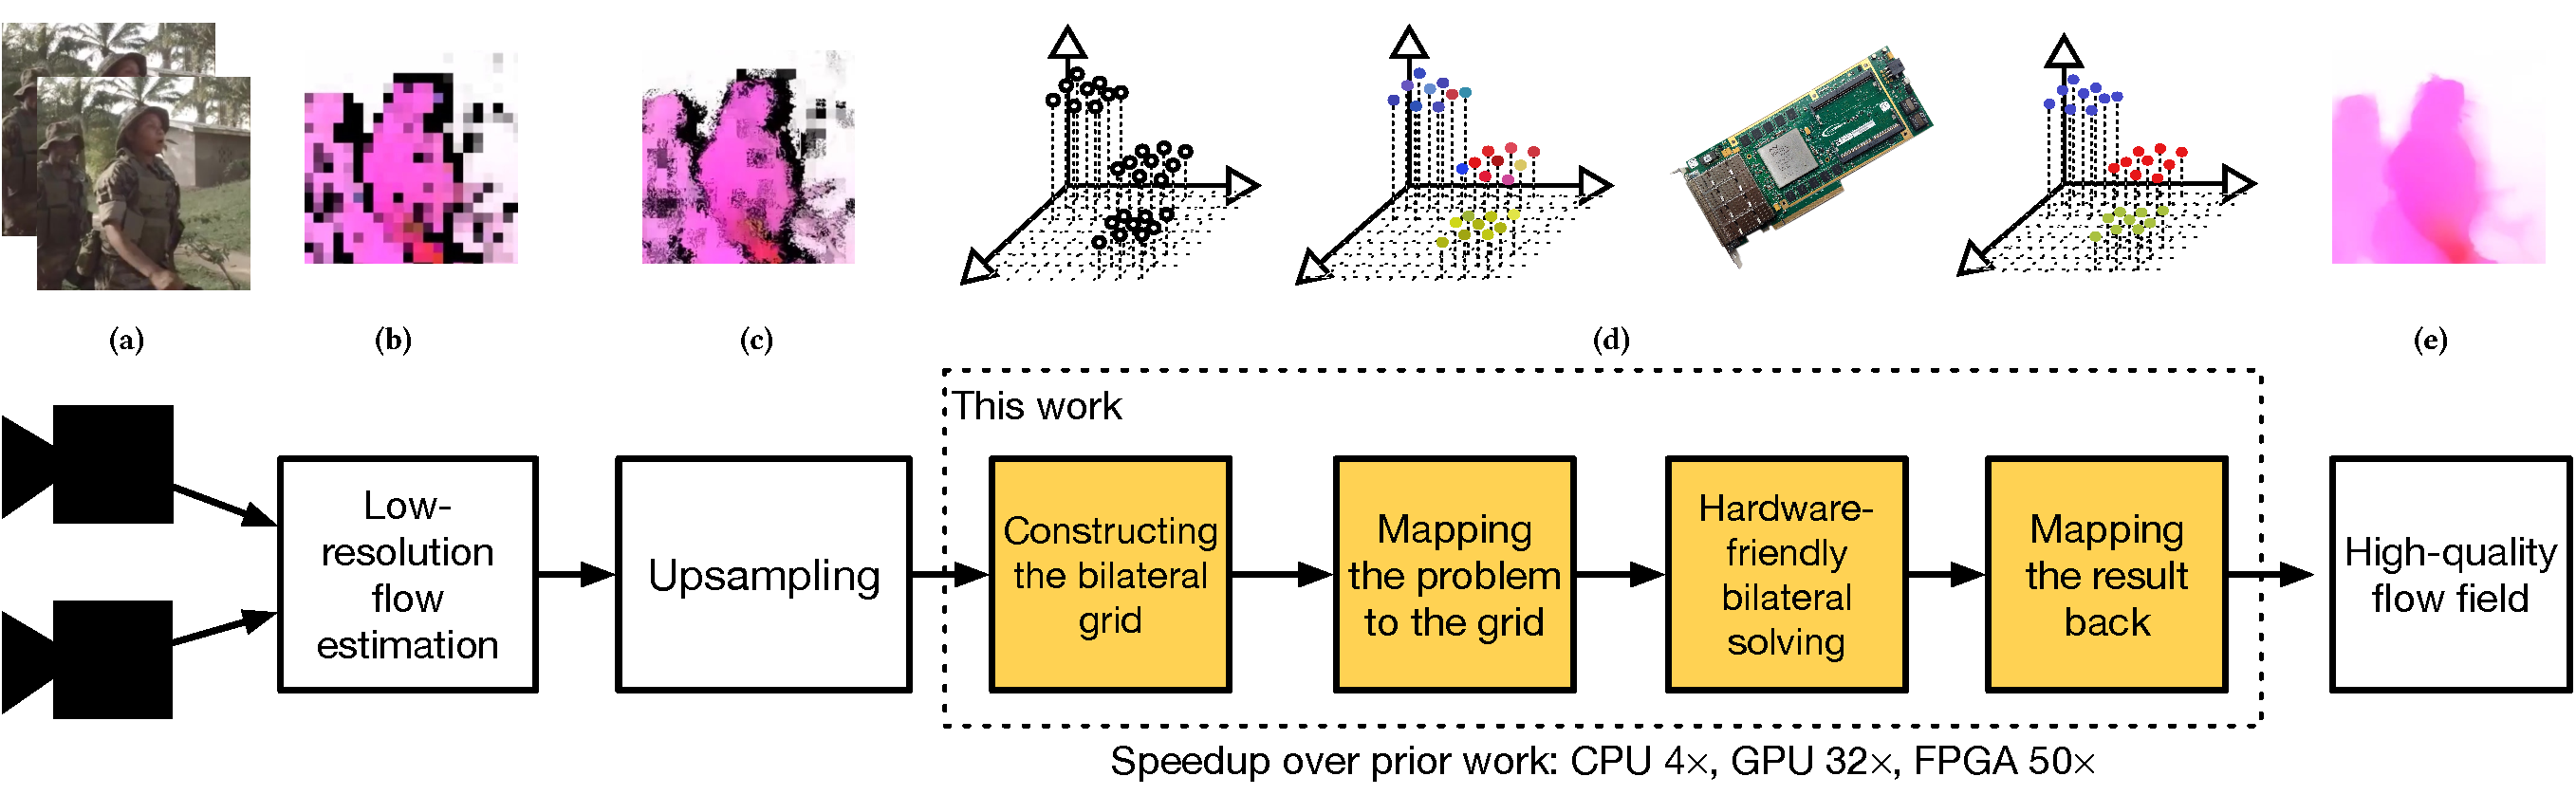
\includegraphics[width=\columnwidth]{hfbs-figs/depth_estimation_steps.pdf}
  \caption{Our bilateral solver produces smooth, edge-aware flow fields.  Given an input pair of images (a), a low-resolution flow is estimated (b),  upsampled to a noisy high-resolution flow (c), and processed with the bilateral solver (d)  to produce an edge-aware smoothed flow (e). Our algorithm for bilateral solving is better-suited for hardware acceleration and results in speedups of up to 50$\times$ over prior work \cite{googlejump, BarronPoole2016}.}
  \label{fig:teaser}
\end{figure*}

\section{Background: Bilateral Filtering and the Bilateral Grid}

\label{sec:hfbs-background}

We base our design for fast and accurate VR video on a state-of-the-art bilateral-space optimization algorithm, the bilateral solver~\cite{BarronPoole2016}.
The bilateral solver is general-purpose and scalable, and can be applied to the many vision applications: optical flow, stereo, depth superresolution, image colorization, and semantic segmentation.
The bilateral solver can be used as part of an edge-aware optical flow algorithm for VR video, and scales to high resolutions efficiently \cite{googlejump}.

This optical flow algorithm generates a correspondence map from a pair of images by computing a rough flow vector for every pixel (Figure~\ref{fig:teaser}b-c), and then refining that flow field until a cost function has been minimized.
To compute this edge-aware per-pixel flow field, the bilateral solver resamples a coarse flow field into \emph{bilateral-space} (Figure~\ref{fig:teaser}d), and then solves an optimization problem in bilateral-space to infer the smoothest possible flow-field that is similar to the input coarse flow field.
In bilateral-space, simple local filters are equivalent to costly, global, edge-aware filters in pixel-space---consequently, flow refinement in bilateral-space is much faster than its pixel-space equivalent.
We perform optimization in a three-dimensional \emph{bilateral grid} data structure \cite{Chen2007}.

Figure~\ref{fig:teaser} describes how we map our optical flow problem to the bilateral solver. We first compute a coarse, tile-based flow field, shown in Figure~\ref{fig:teaser}b, and then upsample it to noisy flow field. As seen in the figure, the upsampled flow in Figure~\ref{fig:teaser}c is very noisy, so we use the bilateral solver to smooth our noisy flow field while maintaining information . This last step (shown as a dotted box in Figure~\ref{fig:teaser}) translates into a computation-intensive optimization problem since multiple factors must be considered.

\begin{figure*}
\centering%
\center
\includegraphics[width=\textwidth]{hfbs-figs/bilateral_grid_3d.pdf}
\caption{Smoothing a noisy flow field in (a) regular 2D space and (b) bilateral space. Regular smoothing produces undesirable artifacts at edges as the flow values blur together. The bilateral grid allows edge-aware smoothing and produces a correct denoised output.}%
\label{fig:bilateral_grid_3d}%
\end{figure*}

To solve the optimization problem, the bilateral solver resamples the problem into \emph{bilateral space}, which is a multi-dimensional space that allows edge-aware operations to be performed on an image.
Figure~\ref{fig:bilateral_grid_3d} illustrates a simplified version of bilateral space and its use in our problem.
We begin with the noisy flow field of Figure~\ref{fig:bilateral_grid_3d}a-i, where color corresponds to some flow value.
If we attempt to denoise this noisy flow field by applying a simple smoothing kernel, the result will present undesirable blurring at color edges.
In Figure~\ref{fig:bilateral_grid_3d}a-ii, for instance, the green region is successfully denoised, but the blue and red regions (which likely belong to different objects) blend around the edges, producing incorrect flow values there.


To smooth this flow field while maintaining sharp edges, we map the problem to bilateral space.
First, we construct a \emph{bilateral grid} for the original image, where a pixel in the image at location $(x,y)$ with luminance $l$ corresponds to a grid block at location $(x,y,l)$ (Figure~\ref{fig:bilateral_grid_3d}b-i, b-ii).
In the 3D bilateral space, the lighter pixels are separated from neighboring darker pixels.
We then map the flow value of each pixel (Figure~\ref{fig:bilateral_grid_3d}b-iii) to its corresponding grid location (Figure~\ref{fig:bilateral_grid_3d}b-iv).
When we smooth this noisy flow in bilateral space, the blue and red areas are no longer neighbors and do not affect each other's value.
Finally, we map the smoothed 3D flow (Figure~\ref{fig:bilateral_grid_3d}b-v) back to the 2D representation (Figure~\ref{fig:bilateral_grid_3d}b-vi).
The resulting  bilateral-smooth output in Figure~\ref{fig:bilateral_grid_3d}a-vi retains sharp edges.

\section{Hardware-Friendly Bilateral Solving}
\label{sec:solver}

In this section, we formulate a bilateral solver that maintains speed, scalability, and accuracy, while also being parallelizable.
We first describe the original bilateral solver of~\cite{BarronPoole2016}, and motivate the requirements for a hardware-friendly bilateral solver. We then provide a detailed formulation of our algorithm and its advantages.

\subsection{Bilateral-Space Optimization}
The original bilateral solver (OBS) consists of (1) an objective and (2) optimization technique~\cite{BarronPoole2016}.
The input to the solver is a reference RGB image, a target image that contains noisy observed quantities we wish to improve, and a confidence image.
The goal is to recover an ``output'' vector $\mathbf{x}$, which will resemble the input target where the confidence is large while being smooth and tightly aligned to edges in the reference image.
To achieve this, Barron and Poole construct an optimization problem of the following form:
\begin{align}
  \underset{\mathbf{x}}{\mathrm{minimize}} &\,\, \frac{\lambda}{2} \sum_{i, j} \hat W_{i,j} \left(x_i - x_j \right)^2  + \sum_i c_i (x_i - t_i)^2
\label{eq:pixel_loss}
\end{align}

The first term of the loss encourages that for all pixel pairs $i$ and $j$, the overall difference between their flow values $x_i$ and $x_j$ is minimized if they are neighboring pixels in the bilateral space.
The second term of Eq.\ref{eq:pixel_loss} encourages each pixel $x_i$ to be close to the target input $t_i$ if that pixel's confidence $c_i$ is high.

The affinity matrix $\mathbf{\hat W}$ is a \emph{bistochastized} (all rows and columns sum to 1) version of a bilateral affinity matrix $\mathbf{W}$.
Each element of the bilateral affinity matrix $W_{i, j}$ describes the affinity between pixels $i$ and $j$ in the reference image in the YUV colorspace:

\begin{align}
W_{i,j} = \exp\left( - { \frac{ \norm*{ \left[ p^x_i, p^y_i \right] - \left[ p^x_j, p^y_j \right] }^2 } { 2 \sigma_{xy}^2 } } -  { \frac{ \left( p^l_i - p^l_j \right)^2 }{ 2 \sigma_{l}^2 } } -  { \frac{\norm*{ \left[ p^u_i, p^v_i \right] - \left[p^u_j, p^v_j \right] }^2 }{ 2 \sigma_{uv}^2 }} \right)
\label{eq:bilateral_affinity}
\end{align}

where $p_i$ is a pixel in the reference image with location $(p^x_i, p^y_i)$ and color $(p^l_i, p^u_i, p^v_i)$.
The $\sigma_{xy}$, $\sigma_{l}$, and $\sigma_{uv}$ parameters control the support of the spatial, luminance (luma), and chrominance (chroma) components of the filter.
Bistochastization normalizes this affinity matrix while maintaining symmetry~\cite{Barron2015A}.

Bilateral operations (e.g., filtering) can be sped up by treating the filter as a ``splat/blur/slice'' procedure in the bilateral grid.
The splat/blur/slice filtering approach corresponds to a compact factorization of $\mathbf{W}$:
\begin{equation}
\mathbf{W} = \mathbf{S}^\mathrm{T} {\mathbf{B}} \mathbf{S} \label{eq:factorization}
\end{equation}
where $\mathbf{S}$ and $\mathbf{S}^\mathrm{T}$ are splatting and slicing, and $\mathbf{B}$ is a $[1$ $2$ $1]$ blur kernel. As in ~\cite{BarronPoole2016},
$\mathbf{S}$ defines a per-pixel mapping from a pixel to a coarse bin in the bilateral grid, where that mapping is a function of the $x$ and $y$ coordinates, $l$ luma, $u$ and $v$ chroma of that pixel.
Multiplying by $\mathbf{S}$ is a data-dependent histogramming operation, and multiplying by $\mathbf{S}^\mathrm{T}$ is a data-dependent interpolation.
The bilateral space optimization formulation of~\cite{Barron2015A} performs bistochastization by calculating two matrices $\mathbf{m}$ and $\mathbf{n}$ that satisfy the following:
\begin{equation}
\hat{\mathbf{W}} = \mathbf{S}^\mathrm{T} \operatorname{diag}\left( \mathbf{n} \over \mathbf{m} \right) \mathbf{B} \operatorname{diag}\left( \mathbf{n} \over \mathbf{m} \right) \mathbf{S} \label{eq:equiv}
\end{equation}
where $\hat{\mathbf{W}}$ is a bistochastic version of matrix $\mathbf{W}$.
The vectors $\mathbf{m}$ and $\mathbf{n}$ describe a normalizing transformation required by the solver.

Barron and Poole also perform a variable substitution \cite{BarronPoole2016}, transforming the high-dimensional pixel-space optimization problem into one with lower-dimensional bilateral-space vertices:
\begin{equation}
\mathbf{x} = \mathbf{S}^\mathrm{T} \mathbf{y} \label{eq:substitution}
\end{equation}
where $\mathbf{y}$ is a small vector of values for each bilateral grid vertex, and $\mathbf{x}$ is the large vector of values for each pixel.

Equations~\ref{eq:factorization} and \ref{eq:substitution} allow us to reformulate the pixel-space loss function of Eq.~\ref{eq:pixel_loss} into bilateral-space in a quadratic form:
\begin{align}
& \underset{\mathbf{y}}{\mathrm{minimize}} \quad  {1 \over 2} \mathbf{y}^\mathrm{T} \mathbf{A} \mathbf{y} - \mathbf{b}^\mathrm{T} \mathbf{y} + c \label{eq:quad_min} \\
&\quad \mathbf{A} = \lambda ( \operatorname{diag}(\mathbf{m}) - \operatorname{diag}(\mathbf{n}) \mathbf{B} \operatorname{diag}(\mathbf{n})) + \mathrm{diag}(\mathbf{S} \mathbf{c}) \nonumber \\
&\quad \mathbf{b} = \mathbf{S} ( \mathbf{c} \circ \mathbf{t} ) \quad\quad c = {1 \over 2} (\mathbf{c} \circ \mathbf{t})^\mathrm{T} \mathbf{t} \nonumber
\end{align}
where $\mathbf{y}$ is the solution to the problem in bilateral-space, $\mathbf{m}$ and $\mathbf{n}$ are defined by Eq.~\ref{eq:equiv}, and $\mathbf{t}$ and $\mathbf{c}$ are per pixel initial solutions and confidences (Eq.~\ref{eq:pixel_loss}).
The Hadamard (element-wise) product is denoted by $\circ$.
%%



The optimization problem of Eq.~\ref{eq:pixel_loss} is intractably slow to solve naively. However, the bilateral-space formulation allows feasible and fast execution.
Minimizing Eq.~\ref{eq:quad_min} is equivalent to solving a sparse linear system:
\begin{equation*}
\mathbf{A}\mathbf{y} = \mathbf{b}
%\label{eq:linear_system}
\end{equation*}
and we can produce a pixel-space solution $\mathbf{\hat x}$ by slicing out the solution from the linear system:
\begin{equation}
\mathbf{\hat x} = \mathbf{S}^\mathrm{T}(\mathbf{A}^{-1} \mathbf{b})
\label{eq:solution}
\end{equation}

In summary, OBS takes an input image vector and a confidence image to construct a simplified bilateral grid from the reference image. With that, it produces the $\mathbf{A}$ matrix and $\mathbf{b}$ vector of Eq. ~\ref{eq:quad_min} to solve the linear system in Eq. ~\ref{eq:solution} and obtain an output image.

\subsection{Algorithmic Modifications}\label{sec:alg_mod}
Though computationally efficient, OBS as presented has a number of properties that make it difficult to implement in hardware, or even to achieve real-time operation on modern CPU or GPU systems.
Vectorizing and parallelizing CPU or GPU processing on the sparse 5D bilateral grid $\mathbf{\hat W}$ demonstrates too-irregular memory access patterns to achieve large performance benefits from parallelization.
Moreover, the use of second order global optimization limits the level of parallelism we can extract from the algorithm.
We modify OBS to construct a hardware-friendly bilateral solver and address these specific challenges: color and sparse memory indexing, and second order global optimization.
Our modifications also allow for an alternative, more efficient initialization and reduced quantization artifacts, which we will discuss after formulating our algorithm.

\paragraph{Color and sparse memory indexing.}
The bilateral solver of~\cite{BarronPoole2016} was designed around a hard bilateral grid or a permutohedral lattice \cite{Adams2010}, meaning that optimization takes place in a ``sparse'' five-dimensional bilateral space (where the five dimensions are position in $x$ and $y$, pixel luma, and two pixel chroma values).
The resulting 5D grid has an image-dependent ``sparsity'' that is challenging to exploit in parallel algorithms.
Moreover, the connectivity structure of the graph used in the bilateral solver varies as a function of the input, leading to expensive and unpredictable memory access patterns.
Attempting to resolve this by solely converting the sparse grid into a ``dense'' representation of the 5D space requires a prohibitive amount of memory.
Instead, HFBS ignores the color of the input image and uses a ``dense'' 3D bilateral grid~\cite{Chen2007}, which makes memory indexing predictable and enables further optimizations. Ignoring color this way induces a small decrease in accuracy, as we will demonstrate.

\paragraph{Second order global optimization.}
The numerical optimization in OBS was performed using the preconditioned conjugate gradient method with a Jacobi or Jacobi-like hierarchical preconditioner.
%Conjugate gradient (and most other second-order optimization techniques) can significantly hasten optimization in tasks such as ours by modeling the curvature of the energy surface being optimized, but
Conjugate gradient methods use a global optimization step: at each iteration, updating each variable of the optimization vector requires reasoning about the gradient at all other variables.
Such global communication requirements make parallel hardware implementation difficult, as we want to be able to individually update and optimize any variable in our state space via local communication with the ``neighboring'' variables in our bilateral grid.
To avoid global communication, HFBS performs optimization using gradient descent with momentum (i.e., the ``Heavy Ball'' algorithm), which can be shown to have similar asymptotic performance as conjugate gradient~\cite{polyak1964some}.
This converts an irregular number of global matrix operations into a regular, but larger, number of local updates that are much easier to execute in parallel.

The Heavy Ball algorithm does not naturally accommodate a preconditioner, so we reformulate our optimization problem with a transformation that indirectly applies a Jacobi preconditioner during optimization.
We find that HFBS slightly underperforms the preconditioned conjugate gradient solver of~\cite{BarronPoole2016} and therefore requires roughly twice as many steps for convergence.
However, since each step is significantly faster to compute (roughly 4$\times$ faster on CPU and much faster on GPU/FPGA), we see an overall increase in performance.

\subsection{Formulating a Hardware-friendly bilateral solver}
We now formalize the details of HFBS and how it relates to the original bilateral solver. Both OBS and HFBS minimize an optimization problem of the form of Eq.~\ref{eq:pixel_loss}. In this case, the $t_i$ is the low resolution flow shown in Figure~\ref{fig:teaser}b. We derive the confidence image for these low resolution flow fields by computing normalized sum-of-squared differences.
The resulting confidence is larger for areas that are near each other and match well.

We obtain the weight $\hat W_{i,j}$, which determines the bilateral-space distance between two pixels $i$ and $j$, from a bistochastized version of the matrix $\mathbf{W}$ whose elements are calculated via the following:
\begin{equation}
W_{i,j} = \exp\left( - { \norm*{ [[p^x_i, p^y_i] - [p^x_j, p^y_j] }^2 \over 2 \sigma_{xy}^2 } -  { ( p^l_i - p^l_j )^2 \over 2 \sigma_{l}^2 }  \right)
\label{eq:hfbs-bilateral_affinity}
\end{equation}
where each pixel $p_i$ has a spatial position $(p^x_i, p^y_i)$ and luminance $p^l_i$.
% The $\sigma_{xy}$ and $\sigma_{l}$ parameters control the support of the spatial and luminance components of the bilateral filter, respectively.
While OBS includes color information in $\hat W_{i,j}$ (Eq.~\ref{eq:bilateral_affinity}), HFBS only considers luminance.


%Both OBS and HFBS reformulate the optimization problem of Eq.~\ref{eq:pixel_loss} as a linear system.
%Before getting into the details of this formulation, we explain another difference that exists between OBS and HFBS.
The bistochastization step in ~\cite{BarronPoole2016} requires 10-20 iterations to achieve low error.
To reduce the fixed cost of this step, we use a faster, approximate bistochastization step for initializing the bilateral solver.
Unlike OBS, which fully-bistochastizes $\mathbf{W}$ into $\hat{\mathbf{W}}$,
we construct an approximately bistochastized $\hat{\mathbf{W}}$ (equivalent to one iteration of bistochastization)
that still satisfies the requirements of the bilateral solver:
\begin{align}
\mathbf{m}_0 = \mathbf{S} \mathbf{1}
\quad\quad
\mathbf{n} = \sqrt{ \epsilon + \mathbf{m}_0 \over \epsilon + \mathbf{B} \mathbf{1} } \quad\quad
\mathbf{m}_1 = \mathbf{n} \circ \left( \mathbf{B} \mathbf{n} \right) \label{eq:m_equals}
\end{align}
% where $\circ$ and $/$ denote element-wise multiplication and division.
In OBS, bistochastization is done to convergence, which produces a $\mathbf{n}$ which satisfies $\mathbf{m}_0 = \mathbf{n} \circ \left( \mathbf{B} \mathbf{n} \right)$.
Partial bistochastization requires that we treat this equality as an assignment, thereby constructing $\mathbf{m}_1$ to explicitly obey this constraint (Eq.~\ref{eq:m_equals}). This produces nearly-indistinguishable output while being faster and easier to compute.

Our normalization also differs from OBS by the use of $\epsilon \sim 0.00001$ in the construction of $\mathbf{n}$.
Adding $\epsilon$ to the numerator prevents divide-by-zero later and
ensures that empty grid cells do not propagate information during optimization. Adding it to the denominator prevents the addition of $\epsilon$ in the numerator from biasing the solution towards $0$.
Note that the partial bistochastization step of HFBS is not iterative and does not require any convergence, and thus is significantly faster than the bistochastization step of OBS.

As described earlier, the expensive per-pixel optimization in Eq.~\ref{eq:pixel_loss} can be reformulated to a much more tractable optimization problem inside a bilateral grid. For convenience we will define $\mathbf{B} \mathbf{y}$ (the product of some grid $\mathbf{y}$ with a blur $\mathbf{B}$) as a scaling of and ``diffusion'' of $\mathbf{y}$:
\begin{align}
%\operatorname{blur}(G) &= 2G + \operatorname{diffuse}(G) \\
\label{eq:diffuse} \mathbf{B} \mathbf{y} &= 2 \mathbf{y} + \mathbf{D} \mathbf{y} \nonumber\\
 \mathbf{D}\mathbf{y} = D(\mathbf{y}) &= \mathbf{y}(x + 1, y, z) + \mathbf{y}(x - 1, y, z) \nonumber \\
& + \mathbf{y}(x, y+1, z) + \mathbf{y}(x, y-1, z) \nonumber \\
& + \mathbf{y}(x, y, z+1) + \mathbf{y}(x, y, z-1) \nonumber
\end{align}
where $\mathbf{D}$ is a diffusion operator (which we can interchangeably refer to as a matrix and  a function) that replaces each element in $\mathbf{y}$ with the sum of its neighbors. Because our 3D bilateral grid is dense in memory, this diffusion process is a simple stencil operation.

We now perform a variable substitution, as in Eq.~\ref{eq:substitution}. For us, this simply requires dividing by the square root of the diagonal of the $\mathbf{A}$ matrix:
%\begin{align}
\begin{equation*}
  \mathbf{y} = \mathbf{p} \circ \hat{\mathbf{z}} \quad \quad  \quad \quad  \mathbf{p} = {1 \over \sqrt{ \mathbf{S} \mathbf{c} + \lambda \left( \mathbf{m}_1 - 2 \left( \mathbf{n} \circ \mathbf{n} \right) \right)}}
  %\mathbf{y} &= \mathbf{p} \circ \hat{\mathbf{z}} \nonumber\\
  %\mathbf{p} &= {1 \over \sqrt{ \mathbf{S} \mathbf{c} + \lambda \left( \mathbf{m}_1 - 2 \left( \mathbf{n} \circ \mathbf{n} \right) \right)}} \nonumber
%\end{align}
\end{equation*}
where $\hat{\mathbf{z}}$ is the solution to the substituted problem.

With our variable substitution in place, we can reformulate Eq.~\ref{eq:quad_min}:
\begin{align}
& \underset{\mathbf{z}}{\mathrm{minimize}} \quad {1 \over 2} \mathbf{z}^\mathrm{T} \tilde{\mathbf{A}} \mathbf{z} - \tilde{\mathbf{b}}^\mathrm{T} \mathbf{z} + c  \nonumber \\
& \quad \tilde{\mathbf{A}} = \mathbf{I} -  \operatorname{diag}\left( \mathbf{q} \right) \mathbf{D}  \operatorname{diag}\left( \mathbf{q} \right) \nonumber \\
  & \quad \tilde{\mathbf{b}} = \mathbf{p} \circ  \left( \mathbf{S} \left( \mathbf{c} \circ \mathbf{t} \right) \right) \nonumber \\
& \quad \mathbf{q} = \sqrt{\lambda} \left( \mathbf{n} \circ \mathbf{p} \right) \nonumber
\end{align}

Here $c$ is the same as in Eq.~\ref{eq:quad_min}. Note that the diagonal of $\tilde{\mathbf{A}}$ is $\mathbf{1}$, so optimizing this problem without a preconditioner is the same as optimizing Eq.~\ref{eq:quad_min} with a Jacobi preconditioner. Minimizing this problem requires solving a linear system, undoing our preconditioning variable substitution, and then slicing out a solution:
\begin{equation*}
\hat{\mathbf{z}} = \tilde{\mathbf{A}}^{-1} \tilde{\mathbf{b}}  \quad  \quad \quad \quad
\mathbf{\hat x} = \mathbf{S}^\mathrm{T}\left( \mathbf{p} \circ \hat{\mathbf{z}}  \right)
\end{equation*}

We will solve this problem using the ``Heavy Ball'' method (gradient descent with momentum).
This problem is fully-described by the diffusion operator $D(\cdot)$ and the bilateral grids $\tilde{\mathbf{b}}$ and $\mathbf{q}$.

Algorithm~\ref{alg:heavy} shows pseudocode describing how optimization is performed:

\begin{algorithm}[h]
\caption{Bilateral-Space Heavy Ball Method \label{alg:heavy} \\
\textbf{Input:}
problem description $\{ D(\cdot), \tilde{\mathbf{b}}, \mathbf{q} \}$,
initial state $\mathbf{z}_{\mathrm{init}}$,
step size $\alpha = 1$,
momentum $\beta = 0.9$,
number of iterations $n = 256$.
\\
\textbf{Output:} state after $n$ iterations $\mathbf{z}$ }
\begin{algorithmic}[1]
\State $\mathbf{z} \gets \mathbf{z}_{\mathrm{init}}$
\State $\mathbf{h} \gets \mathbf{0}$
\For{$i = 1 : n$ }
\State $ \mathbf{g} \gets \mathbf{z} -\mathbf{q} \circ D( \mathbf{q} \circ \mathbf{z} ) - \tilde{\mathbf{b}}$
\State $ \mathbf{h} \gets \beta \mathbf{h} + \mathbf{g}$
\State $ \mathbf{z} \gets \mathbf{z} - \alpha \mathbf{h}$
\EndFor
\end{algorithmic}
\end{algorithm}

It can be shown that if the momentum and step size hyperparameters are set correctly, this heavy ball method has the same asymptotic performance as conjugate gradient \cite{polyak1964some}.
Because preconditioning has been absorbed into the problem, performance approaches preconditioned conjugate gradient.
Since the diffusion operator $D(\cdot)$ is a local stencil, the gradient update to $\mathbf{g}$ and the optimization update to $\mathbf{h}$ and $\mathbf{z}$ can be performed efficiently (i.e., vectorized, parallelized, etc).

\paragraph{Better Initialization to Reduce Optimization Iterations}
Our objective function is convex and thus invariant to the initialization $\mathbf{z}_{\mathrm{init}}$, but a better initialization may allow us to converge in fewer iterations. We can achieve this with a simple weighted blur in our bilateral grid.
\begin{equation*}
\mathbf{z}_{\mathrm{init}} = { \operatorname{blur}( \mathbf{S}( \mathbf{c} \circ \mathbf{t}), \sigma_b) \over \mathbf{p} \circ \operatorname{blur}( \mathbf{S}(\mathbf{c}), \sigma_b ) }
\end{equation*}
where $\operatorname{blur}(\mathbf{a}, \sigma_b)$ is a large-support 3D Laplacian blur of $\mathbf{a}$ with a scale of $\sigma_b$:
%\begin{align}
\begin{equation*}
\begin{split}
  & \operatorname{blur}(\mathbf{a}, \sigma_b)(t_x, t_y, t_z) =  \\
  & \displaystyle \iiint_{-\infty }^{\infty } e^{ \left( \frac{-|\tau_x|-|\tau_y|-|\tau_z|}{\sigma_b} \right)}
      \mathbf{a}(t_x-\tau_x, t_y-\tau_y, t_z-\tau_z ) d \tau_x d \tau_y d \tau_z
\end{split}
\end{equation*}
%\end{align}
and $t_x$, $t_y$, and $t_z$ are 3D coordinates.
This can be efficiently implemented as three separable infinite impulse response filters  (i.e., exponential smoothing, forward and backward) in the three dimensions of the grid.
The intuition
behind this initialization is that the solution should be close to $\mathbf{b}$
where the confidence is large and smooth where confidence is small.
We found that this initialization can be implemented efficiently on a CPU and
roughly halves the number of required iterations.

\paragraph{Reduced Quantization Artifacts}
In OBS, slicing can
 introduce ``blocky'' quantization artifacts in the output~\cite{BarronPoole2016}.
This quantization requires post-processing, adding to the computational cost
of running the bilateral solver.
However, HFBS uses a dense and low-dimensional grayscale bilateral grid
which allows us to efficiently slice out of our bilateral grid using trilinear
interpolation. As shown in~\cite{Chen2007}, this produces smooth results
without post-processing. The trilinear interpolation can be done through a weighted slice, where
$\mathbf{S}_{\mathrm{tri}}$ is analogous to $\mathbf{S}$ but with trilinear
weights instead of hard ``one-hot'' assignment:
\begin{equation*}
\mathbf{\hat x} = { \mathbf{S}_{\mathrm{tri}}^\mathrm{T} \left( \mathbf{m}_0 \circ \mathbf{p} \circ \mathbf{\hat z} \right) \over \mathbf{S}_{\mathrm{tri}}^\mathrm{T} \left( \mathbf{m}_0 \right)} \label{eq:soft_slice}
\end{equation*}
By performing a weighted slice according to the per-vertex grid occupancy
$\mathbf{m}_0$ this process produces artifact-free results in comparison to results from OBS, even if trilinear
interpolation is not used in the splatting step. This ``soft'' slicing is only
slightly more expensive than its ``hard'' equivalent, though both forms can be
implemented very efficiently by virtue of being simple gather operations in a
dense bilateral grid.


% \begin{itemize}
% 	%\item Briefly repeat the high-level VR video process
% 	%\item Then mention the depth estimation step is the slowest
% 	%\item Discuss existing algorithms. Basically previous work from Jon's paper, and then mention the benefits of Jon's algorithm.
% 	%\item Why depth estimation is hard? Mention that it has the common tradeoff between quality and speed. Most of existing fast algorithms are not good enough for VR purposes. Most of high-quality algorithms are slow. Jon's algorithm is pretty fast, and meets VR requirements. However, it does not meet real-time constraints.
% 	\item More details of Jon's older algorithm
% 	\item Other applications of Jon's algorithm
% 	\item Baseline speed report (for the old algorithm)
% 	\item ``Compatibility'' with hardware implementation. In other words, say why the original algorithm is not easy to implement in hardware. For instance, sparse matrix representation is not necessarily efficient. Global optimization steps can be troublesome. Not a lot of room for parallel processing.
% 	\item Discuss the new algorithm
% 	\item New math from Jon
% 	\item Why this algorithm fits a hardware implementation better
% \end{itemize}

% Possible figures and tables:
% \begin{itemize}
% 	\item Re-use the high-level block diagram of VR. Include Google Jump and Google Cardboard. Report run time of each block.
% 	\item Illustration of depth estimation from a pair of images. Show flow of two pixel groups.
% 	\item Figure illustrating Jon's depth estimation algorithm steps: block matching, upsampling, smoothing, etc. Report their run time percentage
% 	\item Figure showing Jon's algorithm being used in other applications.
% 	\item Table reporting speed
% \end{itemize}

% As discussed in Section~XX, VR video preparation involves a high-quality depth estimation (DE) step that turns out to be the slowest step of the pipeline. A natural tradeoff exists between the quality and the speed of DE algorithms. Real-time DE algorithms do not meet the quality requirements of VR [refs], while the existing high-quality algorithms are too slow for real-time VR.

% Barron et al. [ref] present a DE algorithm that meets the VR quality requirements and is XX$\times$ faster than algorithms of similar quality. Nevertheless, this algorithm also fails to meet real-time requirements.

\section{Hardware Architecture}

The formulation of HFBS allows for fast bilateral solving on high\hyp{}performance CPUs or GPUs, but the resulting power consumption may prove prohibitively costly for a full system.
FPGA platforms, on the other hand, can demonstrate fast performance with better power efficiency.
This makes them a more suitable target for a system requiring multiple high\hyp{}performance processors in a single chassis that can support processing 16-camera outputs simultaneously.
To demonstrate power and performance efficiency on FPGAs, we co-designed our hardware implementation with the HFBS algorithm.
In addition to the algorithmic optimizations, we apply hardware-specific techniques such as customized variable bitwidths and bilateral-space memory partitioning to enable better performance.

We first discuss the hardware system at a high level, and then our specific design exploration for bitwidth precision and bilateral grid memory layout.
Finally, we describe the hardware-software interface of our design and how we integrate the accelerator into an application.


\subsection{Microarchitectural Design}

We focus on executing the inner loop of Algorithm~\ref{alg:heavy} with custom hardware, and maintaining the higher-level control flow in software.
In this scheme, a software application splats the optimization problem defined in Section~\ref{sec:solver} onto a bilateral grid, and transfers it to the accelerator for iterative solving.
Figure~\ref{fig:sys-overview} shows a high-level overview of how application functionality is distributed across the system.
The figure also illustrates details of our design's microarchitecture.

\begin{figure}[h]
\centering
\includegraphics[width=.5\columnwidth]{hfbs-figs/system_architecture.pdf}

\caption{High-level system overview of our accelerator. Parallel workers process bilateral grid vertices stored in partitioned memory banks.
Neighboring bank access is controlled with MUXes.
}
\label{fig:sys-overview}

\end{figure}

\paragraph{Data transfer process. }The CPU constructs the bilateral grid based on the input reference image and the initial low-resolution solution provided from prior steps.
This data is splatted onto the grid and transferred to the accelerator via direct memory access (DMA).
The transferred data includes $\hat{\mathbf{b}}$, $\mathbf{q}$, and the initial solution $\mathbf{z}_{\mathrm{init}}$ shown in Algorithm~\ref{alg:heavy}.
First-in-first-out queues (FIFOs) buffer data transfers at the input and output of the accelerator.
During transfer, the memory controller of Figure~\ref{fig:sys-overview} interleaves the data corresponding to each bilateral grid vertex, and partitions the data into memory banks.
After the data transfer is complete, a pool of parallel workers iteratively solve the optimization problem by running the loop of Algorithm~\ref{alg:heavy}.
Multiple grid vertices are processed in parallel and the results are updated in place.
After some number of iterations (we chose 256 iterations for our experiments to ensure convergence), the CPU reads back the final solution and slices it into a 2D result.

\begin{figure}[h]
\centering
\includegraphics[width=.5\columnwidth]{hfbs-figs/worker_microarchitecture.pdf}

\caption{Block diagram of a single worker in our design.
Each worker receives the data for a grid vertex's stencil computation through an input FIFO, processes the grid vertex, and then sends the result out through an output FIFO.
}
\label{fig:microarch-single-worker}

\end{figure}



\begin{figure}[h]
\centering
\includegraphics[width=.5\columnwidth]{hfbs-figs/worker_scaling.pdf}
\caption{Performance scales almost linearly with increased numbers of workers.}
\label{fig:worker-perf}
\end{figure}

Each worker (shown in in Figure~\ref{fig:microarch-single-worker}) performs the inner loop of Algorithm~\ref{alg:heavy} on one grid cell.
It computes the result by streaming in the data from the neighboring cells (required for the ``blur'' operation), as well as the normalization factors required for the optimization process.
For each grid cell, a total of 6 add/subtract operations and 3 multiplications are performed. The updated result is written back to the memory.
The workers compute their local stencil operations synchronously, interfacing primarily with an assigned memory bank and occasionally the neighboring memory banks to access grid blocks that may be stored across banks.
Because each worker executes in lockstep, there are no memory collisions when accessing data in other banks.
Figure~\ref{fig:sys-overview} demonstrates how multiplexers, managed by the main controller, shepherd access to neighboring banks.
As we scale the number of workers, we find that parallelism introduces a 1\% reduction in speedup against perfect linear scaling.
This near-linear scaling can entirely be attributed to our inclusion of the ``Heavy Ball'' algorithm in HFBS, which allowed our design to use only local-neighbor communication rather than global synchronization after each iteration.


Ideally, we want the memory to be partitioned along one grid dimension only, to simplify the neighbor connections between the workers (i.e., simplify the MUXes in Figure~\ref{fig:sys-overview}).
However, this limits the number of parallel workers, to the number of grid blocks along the selected dimension.
If more parallel workers are necessary, the memory should be partition along multiple dimensions, leading to a more complicated neighbor connections.



\paragraph{Number of workers}
The number of workers is affected by several parameters such as run time requirements, power budget, and available resources. Assuming we want the fastest design and have not power constraint, the number of workers will be determined by the available FPGA resources including digital signal processing units (DSPs), look-up tables (LUTs), and memory banks.

  \begin{figure}[h]
		\centering
		\includegraphics[width=.5\columnwidth]{hfbs-figs/fixed_point.pdf}
		\caption{MSE of fixed-point implementations at varied fractional widths, for different bitwidths. MSE is reported relative to 32-bit floating-point. We chose a configuration with 31 bits of fractional precision to reduce chance of overflow in the integer portion.}
		\label{fig:fixed-point}
  \end{figure}

  \begin{table}[h]
		\centering
		\caption{Worker resource utilization and maximum workers at varied bitwidths. Reported MSE is relative to 32-bit floating-point.}

		\begin{tabular}{l|lll}
		\toprule
		Bitwidth        & 32                   & 47                    & 64                   \\ \midrule
		DSPs per Worker & 1                    & 4                     & 16                   \\
		Maximum Workers & 6840                  & 1710                    & 427                   \\
		Min. MSE        & $8.30\times 10^{-4}$ &  $6.69\times 10^{-7}$  & $7.16\times 10^{-13}$ \\ \bottomrule
		\end{tabular}
		\label{table:dsp-workers}


  \end{table}


\paragraph{Fixed-point Conversion} To improve resource utilization, we converted the algorithm from floating-point to fixed-point number representation.
We first implemented our workers using single-precision floating-point, like our CPU and GPU implementations.
We found that the large number of digital signal processing units (DSPs) required for a single floating-point multiplier prohibitively limited the number of workers we could employ, and consequently, the amount of parallelism.
Converting FPGA designs from floating-point to fixed-point number representation resolves this by reducing the resource requirements of hardware multipliers.
Using the cheaper fixed-point multiplier, however, required us to evaluate three competing tradeoffs: (1) the bitwidth of our fixed-point numbers, (2) the precision at a given bitwidth for the integer and fractional portions of the number, and (3) convergence of the solver.
If less than $12$ bits were used for the integer portion, the bilateral grid data would quickly populate with overflow values.
If less than $24$ bits were used for the fractional component of the number, the bilateral solver would not converge, because grid vertices would not have enough precision to capture the change in a value after blurring.
These constraints prevented us from using 32-bit fixed-point numbers, as highlighted by the high mean squared error (MSE) shown in Figure~\ref{fig:fixed-point} across integer-fraction-ratio configurations.
We delineate a maximum error threshold of $\sim 0.00001$, because any errors exceeding that precision eliminate the positive benefits of using an $\epsilon$-value to reduce zero-propagation.
Qualitatively, we also observed that a low MSE correlated with visually similar solver output that converged at the same rate as a 32-bit floating-point solver.
Using 64-bit fixed-point numbers resulted in very low MSE, but, as seen in Table~\ref{table:dsp-workers}, required 16 DSPs per worker, limiting the number of parallel workers we could deploy with these configurations.

As a compromise, we evaluated a 47-bit number representation that was more accurate than 32-bit fixed-point, with 75\% less DSPs than 64-bit fixed-point.
To maintain some precision of 64-bit numbers during non-multiplier arithmetic, we chose a 64-bit fixed-point representation with 15 bits of integer precision and 48 bits of fractional precision, and cast it to and from 47-bit for multiply operations only.
Before multiplying two 64-bit numbers, we round off the bottom 16-bits of each number, resulting in the 1-bit sign, 15-bit integer, 31-bit fraction number highlighted in Figure~\ref{fig:fixed-point}.
We zero-extend the resulting 47-bit output back to a 64-bit number for the rest of the computation.
This fixed-point configuration has a MSE of $3.17\times10^{-7}$ compared to the floating-point implementation, resulting in negligible accuracy loss at the solver output, and the solver converges at the same number of iterations.


\subsection{Bilateral Grid Storage and Memory Layout}

\paragraph{Grid storage size's impact on quality.} Instead of a simple filter like moving average, BSSA maps a noisy depth map to a bilateral grid, refines the depth map by solving an optimization problem, and remaps the bilateral-grid result to pixel-space. Varying the number of pixels that map to a grid vertex impacts the time to compute the stereo refinement for a frame, and also the quality of the depth map. Figure~\ref{fig:vr-res-qual} demonstrates the tradeoff between stereo image quality and bilateral grid size to be processed for high-resolution input images.

\begin{figure}[h]
\centering
    \begin{center}
\includegraphics[width=.45\textwidth]{nsp-figs/vr_res_qual.pdf}
    \end{center}
    \caption{Using a smaller bilateral grid is cheaper to compute but degrades the quality of the output depth map, even at high image resolutions. }
    \label{fig:vr-res-qual}
\end{figure}

Here, we scaled bilateral grid sizes from 4 pixels-per-grid-vertex to 64 in each of three dimensions in a bilateral grid and evaluated the resulting impact on quality using MS-SSIM~\cite{msssim}. We find the resolution of the input images is less impactful than choosing an appropriate grid size to balance quality and computational complexity.

\paragraph{On-chip memory layout.}
To take advantage of block RAM distribution on the FPGA, we partitioned the bilateral grid into chunks along different dimensions, and dedicated grid workers for each partition.
For large, finely divided grids with many vertices (the largest grids we consider have up to 5 million vertices), we could achieve full resource utilization simply by partitioning the grid along one dimension and allocating a single worker to process each memory bank.
For more coarse grids, we partitioned the memory in multiple dimensions.

Our method for laying out data in memory consists of storing all the data needed for a grid vertex in a single packet, and writing the packets sequentially in memory.
Rather than storing multiple bilateral grid data structures separately and repeatedly indexing into each of them to process a single vertex, we interleave the data structures together to access all the information for processing a grid vertex as a single packet.
When a worker is assigned a grid vertex to process, it can fetch most of the data required for its computation from a single partition, including neighboring vertex data for some dimensions.
For large grids, where we only partition on one dimension, the data for two of the three dimensions is stored in the same memory bank, and the worker only has to communicate across banks for the two neighbors in other partitions.
For smaller grids, where we partition along multiple dimensions to improve parallelism, workers may need to fetch more of their neighbors from neighboring partitions.
All inter-bank communication is handled via the main controller of Figure~\ref{fig:sys-overview}.

To aid in fetching grid vertex data for a worker's vertex or neighboring ones, we abstracted this memory layout into a simple addressing method: we dedicate $\lceil\log_2(k)\rceil$ bits of address space for each grid dimension with size  $k$, and use the last three bits to index into the packet for a grid vertex.
For instance, with a bilateral grid of shape $\big[ 247, 166, 16\big]$ partitioned on the first dimension only, a worker assigned the address \texttt{0b 00001010 10100001 0100 001} would map the first dimension's value to memory bank $10$, and use the second and third dimensions to fetch the second item in the packet for grid vertex $\big[ 10, 161, 4\big]$.
Indexing into a neighboring vertex in any dimension means incrementing or decrementing a dimension's tag; the main controller detects when a worker is requesting an address in a neighboring bank and multiplexes the request appropriately.
This discrete mapping of grid dimensions to address spaces results in simple logic for memory addressing, but at the cost of wasted memory space.
Each grid vertex packet contains five items but requires the memory space for eight.
The same is true at the grid partition level, since the number of grid vertices along a dimension is a function of the image resolution and the $\sigma_{xy}$ or $\sigma_{l}$, and does not often fit nicely in power-of-two partitions.



\subsection{FPGA Implementation}

To invoke the bilateral solver accelerator in an application, the application sends a bytestream of bilateral grid data over the FPGA's PCIe-to-AXI DMA interface.
Once the accelerator finishes processing the bilateral grid, it sends the data back in a bytestream to the program over the same interface.
The FPGA's driver can be invoked with standard Unix I/O system calls like $read()$ and $write()$, and can thus be integrated with software applications written in any high-level language.

Some parameters of our design are fixed at configuration time, while others can be modified by software.
At configuration time, we fix the number of grid workers, memory size, and partitioning based on a chosen set of parameters for image resolution and bandwidths in the luma and spatial dimensions.
The parameters essentially define the maximum memory size and number of partitions, which can be interpreted as the upper bound of grid sizes that can be run under a certain configuration.
The bilateral grid dimensions and number of iterations are software-defined at program runtime.
Before an application sends a bilateral grid to the accelerator for processing, it first sends these software-defined parameters.
If the program requests to process a grid too large for the FPGA's configuration, the accelerator will return an error.
This level of flexibility in our design allows applications to process images of varied resolutions at varied grid bandwidths, but can result in wasted resources if the grid size being processed is much smaller than the accelerator's configured grid size.


% !TEX root = paper.tex

\subsection{Experimental Methodology \& Results}
We designed HFBS with the goal of improving bilateral solver performance by parallelizing on modern hardware, while maintaining comparable visual accuracy. 
We compare our algorithm across CPU, GPU, and FPGA implementations. 
The CPU is a Xeon E5-2620 with six cores, and the GPU is an NVIDIA GTX 1080 Ti.
Both platforms execute optimized implementations of the kernels written and tuned with Halide~\cite{halide}.
We prototyped our FPGA design on two devices, and simulated a third. 
To evaluate performance and host-device memory traffic, we experimentally prototyped on a Xilinx Zynq-7020 SoC and  a Xilinx Kintex-7 connected to a host CPU over PCIe.
We also synthesized and simulated a target evaluation design for the Xilinx Virtex UltraScale+ VU9P to evaluate full-resolution frame processing.
Details of each platform are listed in Table~\ref{evaluated-platforms}.

\begin{table}[h]
\centering
\caption{Evaluated platforms}
\begin{tabular}{@{}llrrr@{}}
\toprule
Platform & Type & Cores & Process (nm) & Freq (MHz) \\ \midrule
Xeon E2620 & CPU & 6 & 32 & 2000 \\
Nvidia 1080 TI & GPU & 3584 & 16 & 1582 \\
Zynq SoC & FPGA & N/A & 28 & 125 \\
Kintex Ultrascale+ & FPGA & N/A & 16 & 250 \\
\bottomrule
\end{tabular}
\label{evaluated-platforms}
\end{table}

Both FPGA-based accelerator systems use DMA, either over an on-chip interconnect for the Zynq or PCIe for the Kintex devices. 
The CPU prepares the bilateral-grid data structure with pixels mapped to grid vertices, and transfers them via DMA to the FPGA fabric. 
The hardware accelerator processes the vertices with the bilateral-space filtering and streams them back to the CPU, where the bilateral-grid-filtered result is converted into the fully-processed depth map.

Applying the computation of $B_3$ to a high-resolution video is equivalent to applying millions of blurs to the bilateral grid representation of the video frames. Across a single frame, most of these filters can run in parallel, so we designed streaming compute units to run bilateral filters on a stream of grid vertices. We find that BSSA requires at least 32-bit floating-point precision to produce high-quality depth maps, and use DSP units on the FPGA fabric to compute efficient floating-point operations. Each compute unit requires 18 DSP units in our design, so we can scale up to 12 parallel compute units on the ZC702. However, we project that if we scale up to a top-of-the-line Xilinx Virtex UltraScale+ FPGA, we can parallelize up to 682 compute units, which are more than enough for real-time operation. Table~\ref{table:vr-resources} summarizes the setup we use in our evaluation and resource requirements for real-time performance with a 16-camera system.

\begin{table}[h]
  \centering
\caption{Requirements for FPGA acceleration platform.}
  \begin{tabular}{ l @{\hskip 6pt}l @{\hskip 6pt}l @{\hskip 6pt}l  }
\toprule
 & \textbf{Resource} & \textbf{Evaluation} & \textbf{Target} \\
\midrule
System   & FPGA Model       & Zynq-7000 & Virtex UltraScale+ \\
         & FPGA (\#)        & 1                 & 16                       \\
         & Cameras          & 2                 & 16                       \\
         % & Camera Model     & GoPro HERO4 Black & GoPro HERO4 Black        \\
         % & Image Resolution & 3840x2160         & 3840x2160                \\
         % & Camera FPS       & 30                & 30                       \\
\midrule
Per FPGA & Logic            & 46\%           & 44\%                  \\
         & RAM              & 7\%            & 99\%                  \\
         & DSP              & 94\%           & 100\%                  \\
         & Clock (MHz)      & 125               & 250       \\
\bottomrule
\end{tabular}


\label{table:vr-resources}
\end{table}

\paragraph{Benchmarking.} To benchmark our algorithm, we execute the bilateral solver on flow fields and confidences generated from the ten training images in the Middlebury stereo dataset~\cite{middlebury-data}, and evaluate runtime and accuracy. 
We compare runtimes for our algorithm on CPU, GPU, and FPGA with the bilateral solver of~\cite{BarronPoole2016} on CPU as the baseline.
For CPU and GPU implementations, we report the average runtime from $8$ trials; the FPGA runtime is deterministic and did not vary across trials. 
We characterize power consumption for the CPU and GPU by measuring utilization and scaling from the reported device power.
For the FPGA, we report estimated power consumption from Xilinx Vivado's power report.

\paragraph{Bilateral grid sizes.} The size of the bilateral grid data ranges from 4KB-1.8GB, depending on the $\sigma_{xy}$ used to construct the grid.
All results use a $\sigma_{l} = 16$. 
We use $256$ iterations of optimization in all cases, more than enough guarantee convergence for all algorithms and implementations. 
Note that our performance comparison is not at iso-quality, as our algorithm has slightly more error but qualitatively similar results, which we discuss more in Section~\ref{sec:depth_superres}.
All computation is single-precision floating-point, except for bilateral solving on the FPGA which is conducted with 64-bit fixed-point numbers.
We observe transfer throughput for the FPGA over a single PCIe channel to range between 9.6-11.3 Gbps, which is in keeping with reported estimates.
Since both GPU and FPGA communicate with the host over PCIe and we assume frames can be pipelined, we omit the transfer time between the host processor and the device from reported runtimes.



\subsubsection{Experimental Results}

We now evaluate the performance of our algorithm and hardware, including runtime comparison, power consumption measurements, and accuracy evaluation.

\paragraph{Runtime Results}

Figure~\ref{fig:latency-all} plots the runtime results of bilateral solver implementations on all our benchmarks, as a function of the spatial bandwidth.
Figure~\ref{fig:latency-all}a shows the runtime for the optimization portion of the solver, and Figure~\ref{fig:latency-all}b shows the runtime for the complete bilateral solver including pre-processing.

  \begin{figure}[h!]
    \includegraphics[width=0.235\textwidth]{hfbs-figs/runtime_opt.png}
    \caption{Runtime (Optimization Only)}
  \end{figure}
  \begin{figure}[h!]
    \includegraphics[width=0.235\textwidth]{hfbs-figs/runtime_total.png}
    \caption{Runtime (Total)}
  \end{figure}
% \caption{Runtimes of the baseline, CPU, GPU, and FPGA implementations of HFBS, as a function of the spatial bandwidth ($\sigma_{xy}$ of Eq.~\ref{eq:hfbs-bilateral_affinity}).
% }

% \label{fig:latency-all}
% \end{figure}

As we increase the spatial bandwidth ($\sigma_{xy}$ of Eq.~\ref{eq:hfbs-bilateral_affinity}), we see that the overall grid size decreases, and runtimes shorten for all implementations.
We find that our algorithm outperforms the baseline on all platforms at all spatial bandwidths.
For optimization alone, CPU and FPGA results scale with the grid size, while the GPU results scales until the size of the grid is too small to fully utilize resources.
Because splatting and slicing is not accelerated on the FPGA, runtime for the entire bilateral solver does not scale as well at large grid sizes.

Table~\ref{table:jump_runtimes} highlights the runtime results specifically for the VR Video use-case, where $\sigma_{xy} = 12$ as in~\cite{googlejump}, as well as the power consumption of each hardware configuration. Our algorithm's speed outperforms the CPU baseline on all platforms evaluated, and our FPGA accelerator is significantly faster than the baseline while also reducing power consumption.

\begin{table}[h]
\centering
\caption{Runtimes for different variants of the bilateral solver on different hardware for the VR video use-case. Runtimes for optimization by itself and for the entire algorithm (problem construction/splatting, optimization, and slicing) are shown independently.}


\begin{tabular}{@{}lc@{}cc@{}cc}
\toprule
Algorithm / Platform & \multicolumn{2}{c}{Opt. (ms) } & \multicolumn{2}{c}{Total (ms)} & Power (W) \\ \midrule
 Baseline (CPU) & $1322$ & $\pm 171$ & $2529$ & $\pm 271$ & $16$ \\
                               Our Algorithm (CPU) & $545$ & $\pm 77$ & $588$ & $\pm 77$ & $152$ \\
                         Our Algorithm (CPU + GPU) & $49$ & $\pm 3$ & $78$ & $\pm 5$ & $245$ \\
                        Our Algorithm (CPU + FPGA) & $23$ & $\pm 1$ & $52$ & $\pm 3$ & $25$ \\
\bottomrule
\end{tabular}

\label{table:jump_runtimes}

\end{table}

Note that the CPU-only HFBS runtime reported in Table~\ref{table:jump_runtimes} is still far from the real-time requirement of 30 frames-per-second. The GPU and FPGA implementations get very close to real-time for $\sigma_{xy} = 12$, but still do not make it.
By selecting $\sigma_{xy} = 32$ and losing some accuracy, both FPGA and GPU implementations meet the real-time requirements.

We also observe that HFBS significantly reduces pre-processing. This is mainly caused by the elimination of the Jacobi preconditioner. The switch to a dense 3D bilateral grid improves available parallelism in the splat-slice routines as well.


\paragraph{Computation-communication Tradeoffs}

We consider the throughput of the data output as the ``communication cost'' for offloading, and the cost to compute the pipeline block as the ``computation cost''. We treat the communication cost as fixed for each block; it is simply the cost of offloading the data from each block, as shown in Figure~\ref{fig:vr-data-scale}.

\begin{figure}[h]
\centering
    \begin{center}
\includegraphics[width=.48\textwidth]{nsp-figs/vr_input_data.pdf}
    \end{center}
    \caption{Computation distribution and output data size for blocks in a VR video pipeline (2 of 16 cameras). }
    \label{fig:vr-data-scale}
\end{figure}

For all blocks except disparity refinement, we assume the computation cost to be the compute time evaluated using the ARM CPU baseline's performance numbers. We average the compute time for the disparity refinement block over five executions of the kernel over a frame. Because this processing flow can be pipelined across frames in a video stream, the ``total cost'' of the system can be considered to be dominated by the lowest-throughput block of the system.

Figure~\ref{fig:vr-fps} shows the runtime results of different pipeline configurations, uploaded on a networked connection to a viewing device supporting at least 30 FPS. We seek to uncover scenarios in which both computation and communication surpass our minimum frame rate of 30 FPS---if one or both costs falls below the threshold, the system cannot support real-time operation.

\begin{figure*}[h]
\centering
    \begin{center}
\includegraphics[width=1.0\textwidth]{nsp-figs/vr_compute_transfer.pdf}
    \end{center}
    \caption{Pipeline configurations with different bilateral smoothing implementations (CPU, GPU, FPGA), and resulting upload rates (frames per second). Only the full pipeline with FPGA acceleration can meet a 30 FPS upload requirement.}
    \label{fig:vr-fps}
\end{figure*}


For the first three scenarios, the cost of doing little computation before offloading is cheap, even on the ARM core, but the communication cost for the raw captured data falls short of our 30 FPS threshold. Computing the disparity refinement in $B_3$ is more costly, and the CPU and GPU implementations are not fast enough to support real-time operation. Moreover, the cost of offloading the computed depth maps before image stitching is significantly lower.

The computation cost of image stitching in $B_4$ is marginal compared to BSSA, as well, and the resulting FPS is virtually the same. The data size to communicate after $B_4$, however, is much smaller, as discussed in Figure~\ref{fig:vr-data-scale}, and is the only data size small enough to support real-time uploading. We find that the configuration with all the blocks processed in-camera and $B_3$ mapped to the FPGA is the only configuration where both computation and communication pass the threshold and support real-time processing.

Our analysis indicates that this camera system is primarily constrained by network bandwidth. For our evaluation, we assumed transfer speeds of 25 Gigabit Ethernet. As network connections grow faster, our results will trend towards offloading computation right off the sensor. For instance, at a hypothetical ultra-high-throughput network link of 400-Gb Ethernet, the 16-camera output can be uploaded at 395 FPS, reducing the efficiency incentive for in-camera processing in this scenario.

\paragraph{Depth Superresolution}
\label{sec:depth_superres}

Because our proposed model is an approximation to the bilateral solver, we
should expect some drop in the quality of our output relative to that
of \cite{BarronPoole2016}. To quantify this drop in accuracy, we evaluate on the
depth superresolution task of \cite{ferstl2013b}, which was the primary
evaluation used in \cite{BarronPoole2016}. We evaluate using the same experimental
setup and the same hyperparameters as \cite{BarronPoole2016} ($\sigma_{xy} = 8$, $\sigma_{l} = 4$), and report MSE with respect to ground truth from the Middlebury Stereo Dataset~\cite{middlebury-data}.

\begin{table}[h]
\centering
\caption{Depth Superresolution Task \cite{ferstl2013b}}

\begin{tabular}{@{}lcc@{}}
\toprule
Algorithm & Error (MSE) & Runtime (sec) \\
\midrule
            Chan \etal \cite{chan2008}   &  $ 3.89 $  &  $ 3.02 $   \\
            Min \etal  \cite{Min2014}   &  $ 3.78 $  &  $ 0.383 $  \\
    Domain Transform \cite{Gastal2011}   &  $ 3.60 $  &  $ 0.021 $  \\
           Ma \etal   \cite{Ma2013}   &  $ 3.53 $  &  $ 18 $  \\
        Zhang \etal  \cite{Zhang2014}   &  $ 3.51 $  &  $ 1.346 $  \\
    Guided Filter (Matlab) \cite{He2010}   &  $ 3.51 $  &  $ 0.434 $  \\
        Fast Guided Filter \cite{He2015}   &  $ 3.45 $  &  $ 0.225 $  \\
           Yang \etal  \cite{Yang2015}   &  $ 3.44 $  &  $ 0.304 $  \\
         Farbman \etal \cite{FFLS2008}   &  $ 3.24 $  &  $ 6.11 $  \\
          JBU \cite{Adams2010,Kopf2007}   &  $ 3.19 $  &  $ 1.98 $  \\
        Barron \& Poole \cite{BarronPoole2016}   &  $ 2.75 $  &  $ 0.234 $  \\ \hline
                               Our Model   &  $ 3.27 $  &   $ 0.047 \pm 0.002$ \\
\bottomrule
\end{tabular}

\label{table:depth_superres}
\end{table}

As can be seen in Table~\ref{table:depth_superres}, our model produces a slightly
higher error than that of \cite{BarronPoole2016}, but has a significantly
lower runtime (here we report runtime on a Nvidia 1080 Ti). This increase in error
is due to the fact that our model ignores color in the input image, and so has
difficulty distinguishing between pixels with different chroma but similar
luma. The images in this task are unusually colorful and ``cartoonish'',
by virtue of being a constructed vision task, so this increase in error
represents an upper-bound on the increased error we expect to see in natural scenes.
Even with this reduction in error, we see that
HFBS is significantly faster than all more-accurate techniques, and
significantly more accurate than all faster techniques.

% \begin{figure}[h]
% \centering
%   \subfloat[Input reference image,\\ from \cite{middlebury-data} ]{
%     \includegraphics[width=0.235\textwidth]{hfbs-figs/super_depth/1_image.png}
%     }
%   \subfloat[Input noisy depth,\\ before filtering ]{
%     \includegraphics[width=0.235\textwidth]{hfbs-figs/super_depth/1_bicubic.png}
%     }
%   \subfloat[Improved depth \\ from \cite{BarronPoole2016} ]{
%     \includegraphics[width=0.235\textwidth]{hfbs-figs/super_depth/1_bsqs.png}
%     }
%   \subfloat[Our improved depth \\ (with HFBS) ]{
%     \includegraphics[width=0.235\textwidth]{hfbs-figs/super_depth/1_grayscale_bs.png}

\begin{figure}[!ht]
  \subfloat[Input reference image, from \cite{middlebury-data}]{%
    \includegraphics[width=0.45\textwidth]{hfbs-figs/super_depth/1_image.png}
  }
  \hfill
  \subfloat[Input noisy depth, before filtering]{%
    \includegraphics[width=0.45\textwidth]{hfbs-figs/super_depth/1_bicubic.png}
  }
  \subfloat[Improved depth from \cite{BarronPoole2016}]{%
    \includegraphics[width=0.45\textwidth]{hfbs-figs/super_depth/1_bsqs.png}
  }
  \hfill
  \subfloat[Our improved depth  (with HFBS)]{%
    \includegraphics[width=0.45\textwidth]{hfbs-figs/super_depth/1_grayscale_bs.png}
  }
  \caption{A qualitative comparison of HFBS's performance
  compared to the model of \cite{BarronPoole2016} on the depth superresolution
  task of \cite{ferstl2013b}. HFBS produces similar output to \cite{BarronPoole2016} and is significantly faster.}
  \label{fig:depth_superres}
\end{figure}


We present qualitative results for this task in Figure~\ref{fig:depth_superres}.
As discussed in Section~\ref{sec:alg_mod}, HFBS requires double the iterations to achieve the same accuracy level of OBS, but still performs significantly faster.
We can see that our output depths are qualitatively very similar to those of
\cite{BarronPoole2016}, as expected.

\subsection{Discussion}
There are a number of optimizations our hardware design can integrate for improved performance.
Nevertheless, we observe that our design can be practically deployed at both the camera node or in the cloud to enable real-time VR video rendering.


\paragraph{Accelerator optimizations.}
There are many opportunites to further optimize our hardware design.
For instance, our design only accelerates the iterative optimization portion of HFBS.
Integrating splat and slice operations into our accelerator, as in~\cite{bilat_isscc}, would reduce transfer costs from GB-large bilateral grid to smaller MB-sized images and further reduce runtimes. 
Also, many vertices of the dense bilateral grid begin as zeros and do not need to be processed;  intelligently ignoring these zero-valued grid vertices can reduce wasted computation and potentially improve the runtime. 
Similarly, the wasted memory space from our addressing scheme can be mitigated with increased control logic, which may allow us to maximize the bilateral grid size.
We can also more tightly pipeline the three phases of reading, processing, and writing out grid data to reduce latency; these stages currently execute sequentially.
To ease prototyping portability, our design used single PCIe channels for reading and writing, which leaves the remaining channels idle. 
The board we target, Xilinx Virtex UltraScale+, supports up to 16 PCIe channels that can be leveraged to improve transfer times.

\paragraph{System specifications for real-time VR video processing platforms.}
While our design can execute bilateral solving under real-time constraints, the bilateral solver is just one step in the Jump VR video rendering pipeline. 
Moreover, the design we present processes the flow field from a camera pair while the VR video capture system we target processes 16 flow fields from a 16-camera rig. 
We outline the specifications and cost for a system that could process the full 16-camera input to produce virtual reality video in real-time in Table~\ref{vr-shoebox}. 
\begin{table}[h]
\centering
\caption{Full-system specification for an end-to-end real-time VR pipeline}
\label{vr-shoebox}

\begin{tabular}{llrrrr}
\toprule
\textbf{Item}     & \textbf{Use}          & \textbf{\#} & \textbf{Unit \$} & \textbf{Total \$} & \textbf{Max. Power} \\ \midrule
GoPro      	 & Camera      & $16$   & \$$360$       & \$$5,760$       & N/A            \\ 
Virtex Ultrascale+	 & HFBS   & $16$   &  \$$2,995$    	& \$$47,920$ 		& $\approx$$400$ W   \\
Intel i7-7700K     & Host CPU     	  & $1$     & \$$350$   	& \$$350$         &  $\approx90$ W              \\
Nvidia Titan X    	 & Etc. acceleration  & $1$        	& \$$1,600$       & $\approx$$250$    \\ \midrule 
\midrule \textbf{Full-System} &  & & & \$55,360 & 490 W \\ \bottomrule
\end{tabular}

\end{table}


The monetary cost of deploying such a many-FPGA system in both configurations is high, but the power consumption of our FPGA-based system, with 16 high-end fully-utilized FPGAs, is approximately that of two GPUs.
Such power savings can be critical for mobile camera rigs.
At the data center level, power constraints are less stringent, but deploying custom hardware for high-bandwidth tasks can still reduce power consumption and operating costs.


\subsection{Conclusions}

The hardware-friendly bilateral solver enables scalable, real-time processing of VR video on modern hardware.
We explore a hardware-software codesign approach to construct an algorithm that is both faster \emph{and} more accurate than prior work, optimizing algorithm details and hardware implementation together. 
In particular, HFBS uses a bilateral-space Heavy Ball algorithm and a 3D dense bilateral grid that allows fast and predictable memory accesses. 
In contrast, the baseline algorithm~\cite{BarronPoole2016} uses a 5D sparse grid and is about 4$\times$ slower than HFBS. 
We also design an FPGA accelerator for HFBS using reduced-precision fixed-point numbers and customized memory layout. 
Our CPU, GPU, and FPGA implementations of HFBS are 4$\times$, 32$\times$, and 50$\times$ faster than the original bilateral solver. 
We observe that our FPGA accelerator is more energy-efficient than comparable CPU and GPU implementations, and can be practically deployed at both the camera node or in the cloud to enable real-time VR video rendering.


%************************************************
\chapter{Perceptually-Compressed Video Storage and Streaming}\label{ch:vignette}
%************************************************
\markboth{Perceptually-Compressed Video Storage and Streaming}{Perceptually-Compressed Video Storage and Streaming}

%!TEX root = paper.tex

\newcommand{\videoDataVsStorageFigure}{
\begin{figure}[h]
  \centering
\includegraphics[width=\linewidth]{vignette-figs/storage-video-growth.pdf}
  \caption{Normalized growth of total storage produced and video data captured since 2008~\cite{cisco2016zettabyte,fontana2018storage}. Video data is outgrowing  storage capacity, taxing storage system capacity.}
  \label{plot:video-data-vs-storage}
\end{figure}
}

\newcommand{\tileVsSizeFigure}{
\begin{figure}[h]
  \centering
\includegraphics[width=.6\linewidth]{vignette-figs/tileSizeQuality2.pdf}
  \caption{Compression ratio and PSNR at the optimal number of tiles for each video. The optimal number of tiles is video-dependent, not correlated with quality or compression ratio.}
  \label{plot:tile-vs-size}
\end{figure}
}

\newcommand{\computeTable}{
\begin{table}[h]
\centering
\caption{Mean processing time per video, evaluated over all videos in our datasets.}
\label{table:compute}

\begin{tabular}{lrcrc} \toprule
   & \multicolumn{2}{c}{Exhaustive} & \multicolumn{2}{c}{Heuristic }\\
    \cmidrule(lr){2-3}\cmidrule(lr){4-5}
  Task                       & Time (s) & \%   & Time (s) & \% \\ \midrule
  Generate saliency map      & 1633     & 49\% &  1633     & 95\%   \\
  Compute tile configuration & 1696     & 50\phantom{\%} &  59      & 4\phantom{\%}   \\
  Saliency-based transcode   & 21       & \phantom{0}1\phantom{\%}  &  21      & \phantom{0}1\phantom{\%}   \\ \midrule
  Total                      & 3350     &      &  1713     & \\ \bottomrule
\end{tabular}

\end{table}

}

\newcommand{\userStudyFigure}{

\begin{figure}[h]
  \centering
  \includegraphics[width=.6\linewidth]{vignette-figs/user-study.pdf}
  \caption{Results of perceived quality preference user study, averaged across participants and videos by bitrate. Participants either preferred \name or perceived no difference between 20 Mbps \hevc videos and \name videos at 5--20 Mbps.}
  \label{plot:user-study}
\end{figure}
}
\newcommand{\failureModeFigure}{

\begin{figure}[h]
  \centering
  \includegraphics[width=\linewidth]{vignette-figs/tile-failure.pdf}
  \caption{Two instances of failure from tiling (top-left tile) during fast-motion sequences.}
  \label{fig:vignette-failures}
\end{figure}
}


\newcommand{\vbenchScoreFigure}{
\begin{figure}[h]
  \centering
  \includegraphics[width=\linewidth]{vignette-figs/vbench-scores.pdf}
  \caption{\texttt{vbench} scores comparing \nameCompress to their reference. \todo{fake data}}
  \label{plot:vbench}
\end{figure}
}

\newcommand{\saliencyTilesOverviewFigure}{
\begin{figure}[h]
  \centering
  \includegraphics[width=.6\linewidth]{vignette-figs/tiled-bitrate}
  \caption{Overview of \nameCompress algorithm.}
  \label{fig:saliency-tiles-overview}
\end{figure}
}

\newcommand{\architectureOverviewFigure}{
\begin{figure}[h]
  \centering
  \includegraphics[width=.6\linewidth]{vignette-figs/high-level-architecture}
  \caption{\name provides two features: \nameCompress, a perceptual compression algorithm, and \nameStore, a storage manager for perceptually compressed videos.
  Integrating perceptual information with the storage manager reduces network bandwidth and storage costs.}
  \label{fig:high-level-architecture}
\end{figure}
}

\newcommand{\exampleVidSaliencyFigure}{

\begin{figure*}[h]
  \centering
  % \begin{subfigure}{.32\textwidth}
  %   \centering
  %   \includegraphics[width=.9\linewidth]{vignette-figs/elfuente_in.png}
  %   \caption{Input video frame from Netflix dataset~\cite{netflix2016data}.}
  %   \label{subfig:og-stil}
  % \end{subfigure}%
  % \begin{subfigure}{.32\textwidth}
  %   \centering
  %   \includegraphics[width=.9\linewidth]{vignette-figs/elfuente_sal.png}
  %   \caption{Saliency map, produced by MLNet~\cite{mlnet2016}, overlaid on input.}
  %   \label{subfig:sal-still}
  % \end{subfigure}%
  % \begin{subfigure}{.32\textwidth}
  %   \centering
  %   \includegraphics[width=.9\linewidth]{vignette-figs/elfuente_vignette.png}
  %   \caption{Perceptually-compressed \name video, 85\% smaller at iso-quality.}
  %   \label{subfig:sal-vign}
  % \end{subfigure}%

  \subfloat[Input video frame from Netflix dataset~\cite{netflix2016data}.]{
  \label{subfig:og-stil}
  \includegraphics[width=.275\linewidth]{vignette-figs/elfuente_in.png}
  }
  \qquad
  \subfloat[Saliency map produced by MLNet~\cite{mlnet2016}, overlaid on input.]{
  \label{subfig:sal-still}
  \includegraphics[width=.275\linewidth]{vignette-figs/elfuente_sal.png}
  }
  \qquad
  \subfloat[Perceptually-compressed \name video, 85\% smaller at iso-quality.]{
  \label{subfig:sal-vign}
  \includegraphics[width=.275\linewidth]{vignette-figs/elfuente_vignette.png}
  }
  \caption{Example video still, neural network-generated saliency map, and output \name perceptually compressed video.}
  \label{fig:example-vid-saliency}
\end{figure*}


}


\newcommand{\systemOverviewFigure}{
\begin{figure*}[h]
% \begin{subfigure}{.48\textwidth}
%   \centering
%   \includegraphics[width=.9\linewidth]{vignette-figs/system-overview-open.pdf}
%   \caption{Open-loop offline saliency compression:~\name automatically generates saliency maps to include perceptual data during video transcoding.}
%   \label{fig:system-overview-open}
% \end{subfigure}\hfill%
% \begin{subfigure}{.48\textwidth}
%   \centering
%   \includegraphics[width=.9\linewidth]{vignette-figs/system-overview-closedloop.pdf}
%   \caption{Closed-loop re-compression:~\name~can leverage perceptual cues from VR headsets and other eyetracking devices to improve compression.}
%   \label{fig:sub2}
% \end{subfigure}
\caption{High-level architecture of~\name~system design.}

  \centering
  \subfloat[Open-loop offline saliency compression:~\name automatically generates saliency maps to include perceptual data during video transcoding.]{
    \label{fig:system-overview-open}
    \includegraphics[width=.46\textwidth]{system-overview-open.pdf}
  }
  \qquad
  \subfloat[Closed-loop re-compression:~\name~can leverage perceptual cues from VR headsets and other eyetracking devices to improve compression.]{
    \label{fig:system-overview-closed}
    \includegraphics[width=.46\textwidth]{system-overview-closedloop.pdf}
  }
  \caption{High-level architecture of~\name~system design.}
  \label{fig:system-overview}
\end{figure*}
}

\newcommand{\videoMetadataFigure}{
\begin{figure}[h]
  \centering
  \includegraphics[width=.65\linewidth]{vignette-figs/physical-layout}
  \caption{Physical layout of video metadata in~\lightdb. \name-specific features are highlighted.}
  \label{fig:video-metadata}
\end{figure}
}

% \newcommand{\benchmarkInformationFigure}{
% \begin{figure}[t]
%   \centering
%    \subfloat[Benchmarks used for video profiling]{
%      	\label{table:benchmarks}
%        \resizebox{\linewidth}{!}{%
%        \begin{tabular}{l|l l l l}
%        Type                      & Benchmark & Description & Bitrate (Mbps) & Size (MB)        \\\hline
%        \multirow{2}{*}{Standard} & vbench~\cite{vbench}    & YouTube dataset & 0.53 - 470 & 757  \\
%                                  & Netflix~\cite{netflix2016data}   & Netflix dataset & 52 - 267 & 1123 \\
%        \multirow{2}{*}{VR}       & VR-360~\cite{saliency-map}    & 4K-360 dataset & 10 - 21 & 1400   \\
%                                  & Blender~\cite{blender}   & UHD / 3D movies & 10 - 147 & 6817 \\
%        \end{tabular}
%        }
%      } \\
%  \subfloat[Resolution and entropy distribution]{
%  \label{subfig:benchmark-entropy-res}
%   \includegraphics[width=\linewidth]{resolution-entropy2}
%
%  }
%   \caption{Characteristics of benchmark videos used to characterize \name. }
%   \label{fig:benchmark-info}
% \end{figure}
%
% }

\newcommand{\benchmarkInformationFigure}{
\begin{table}[h]
  \centering
       \begin{tabular}{l l l l l} \toprule
       Type                      & Benchmark & Description & Bitrate (Mbps) & Size (MB)        \\\midrule
       \multirow{2}{*}{Standard} & vbench~\cite{vbench}    & YouTube dataset & 0.53--470 & 757  \\
                                 & Netflix~\cite{netflix2016data}   & Netflix dataset & 52--267 & 1123 \\
       \multirow{2}{*}{VR}       & VR-360~\cite{saliency-map}    & 4K-360 dataset & 10--21 & 1400   \\
                                 & Blender~\cite{blender}   & UHD / 3D movies & 10--147 & 6817 \\ \bottomrule
       \end{tabular}


  \caption{Video datasets used to characterize \name. }
  \label{table:benchmarks}
\end{table}

}


\newcommand{\bitrateLadderFigure}{
\begin{figure}[h]
  \centering
  \subfloat[We varied bitrate and resolution for each video.]{
    \label{fig:bitrate-ladder-all}
    \includegraphics[width=1.05in]{vignette-figs/bitrate-ladders-subset}
  }
  \qquad
  \subfloat[The final bitrate ladder is the convex hull that maximizes PSNR.]{
    \label{fig:bitrate-ladder-max}
    \includegraphics[width=1.4in]{vignette-figs/bitrate-ladders-max}
  }

  \caption{Example bitrate ladder generated for one video in our dataset. We generated resolution-bitrate curves for all videos in our datasets.}

  \label{fig:bitrateladder}
\end{figure}

}

\newcommand{\avgStorageBitrateSavings}{
\begin{figure}[h]
  \centering
    \includegraphics[width=.6\linewidth]{vignette-figs/bitrate-storage-savings}

  \caption{Aggregate storage savings by dataset. \nameCompress reduces videos to 1--15\% of their original size while maintaining PSNR of 34--39 dB and EWPSNR of 45-51 dB.}

  \label{fig:average-storage-bitrate-savings}
\end{figure}

}

\newcommand{\awsBreakevenFigure}{
\begin{figure}[h]
  \centering
    \includegraphics[width=.6\linewidth]{vignette-figs/aws-breakeven}
  \caption{Estimated AWS costs for deploying \name versus traditional video transcoding. \name's additional compute cost is amortized after $\scriptstyle\sim$2 billion video views over a 1-million video library.}

  \label{fig:aws-utilization}
\end{figure}

}
\newcommand{\powerFigure}{
\begin{figure}[h]
  \centering
    \includegraphics[width=.6\linewidth]{vignette-figs/power}
  \caption{Time to dissipate a Google Pixel 2 phone battery from 100\% to 30\% when viewing \hevc and \name videos continuously. \name videos provide 1.67$\times$ longer video playback on mobile phones.}

  \label{fig:power}
\end{figure}

}

%!TEX root = ../paper.tex


For decades, video codecs have exploited how humans see the world, for example, by devoting increased dynamic range to spatial features (low frequency) or colors (green) we are more likely to observe.
One such perceptual cue, \emph{saliency}, describes where in a video frame a user focuses their perceptual attention.
As video resolutions grow, e.g., \threesixty video and 8K VR displays, the salient regions of a video shrink to smaller proportion of the video frame~\cite{sitzmann2018saliency}.
Video encoders can leverage saliency by concentrating bits in more perceptually interesting visual areas.
Prior work, however, focuses only on achieving bitrate reduction or quality improvement at the cost of complicated, non-portable prototypes designed for a single codec implementation \cite{li2011visual,hadizadeh2014vidcomp,8117038,5223506}.
Exploiting saliency in video compression can ease the burden of video data growth while maintaining perceptual quality.
In this work, we address the challenges of storing and integrating this perceptual data into cloud video storage and processing systems.


In this section, we describe \name, a cloud video storage system that leverages perceptual information to reduce video sizes and bitrates.
\name is designed to serve as a backend for large-scale video services, such as content delivery systems or social media applications.
\name has two components: a compression scheme, \textit{\nameCompress}, and a storage manager, \textit{\nameStore}.
\nameCompress leverages a new saliency-based compression algorithm to achieve up to 95\% lower bitrates while minimally reducing quality.
\nameStore uses a simple API to trigger saliency-based compression when needed, allowing applications to trade off between faster traditional compression and \name's smaller video sizes.
The system uses low-overhead metadata, can be easily integrated into existing media storage structures, and remains transparent to standard video applications.
% \nameStore supports generating saliency maps with a neural network as well as integrating perceptual information from VR headsets or other eye tracking devices to improve the quality of its perceptual compression. %, shown in~\ref{fig:system-overview}.
% \todo{do we get power savings?}

\name is \textit{not} a new standalone codec or compression standard.
Instead, it extends existing, modern codecs to take advantage of the untapped perceptual compression potential of video content, especially high-resolution video served in VR and entertainment settings.
% \todo{drop in two examples of situations you'd use \name: video popularity or 360 video players}
% We explicitly designed our saliency-based compression scheme to work with standard codec features.\brandon{Redundant?}
As a result, off-the-shelf software and hardware accelerators can decompress \name's perceptually compressed videos with no modifications.
We implement \name as an extension to \lightdb~\cite{lightdb}, a database management system for video.
Our prototype of \name demonstrates cost savings to cloud video providers and power savings during mobile video playback.
Our work thus complements other advances in codec implementations and can easily be implemented with new standards, like \avone.

This chapter makes the following contributions:

\begin{itemize}
  \item \textbf{Systems support for perceptual video compression.} We propose \name, a system for producing and managing perceptually compressed video data. \name produces videos that are 80--95\% smaller than standard videos, consume 50\% less power during playback, and demonstrate minimal perceived quality loss.
  \item \textbf{A forward-compatible perceptual encoding pipeline.} \name leverages existing features of modern video codecs to implement perceptual compression, and can be deployed in any video processing system that supports such codecs, such as \hevc or \avone. % \hevc-based encoding.
  \item \textbf{Custom storage for perceptual data.} \name's storage manager efficiently stores and manages perceptually compressed videos and is integrated in a modern video processing database system. \nameStore supports both a heuristic-guided search for fast perceptual compression and an exhaustive mode to compute an optimal saliency-based compression configuration.
\end{itemize}

% \noindent\textbf{Quantitative evaluation and user study:}
\noindent To our knowledge, this is the first work to consider storage management of perceptually-compressed video information.
Using saliency as a motivating perceptual cue, we evaluate the limits of perceptual compression in a video storage system with a collection of modern and high-resolution video datasets.
\name's compression scheme uses a neural network trained to predict content saliency and an off-the-shelf \hevc encoder to reduce bitrate requirements by 80--95\%.
Our results show that \name can reduce whole-system power dissipation by 50\% on a mobile phone during video playback.
Quantitative evaluation and user study results validate that these bitrate and power savings come at no perceived loss in video quality.
 %\brandon{Oh, right, here's the evaluation stuff.  Consider moving most of this into a contribution unless this is a normal thing for the conference?}

%!TEX root = ../paper.tex

\section{Background: Perceptual Compression Using Saliency Maps}

\label{sec:saliency}
Saliency is a widely-utilized measure of the perceptual importance of visual information.
Saliency data encodes the perceptual importance of information in a video, such as foreground and background or primary and secondary objects.
Video codecs already use some perceptual information, like motion and luminance, to improve compression performance~\cite{hevc}, but new modes of video viewing (such as with a VR headset) introduce the opportunity to integrate richer cues from the human visual system~\cite{lee2012perceptualcodingsurvey}.
In this paper, we use saliency as an example of one such perceptual cue to demonstrate the potential of perceptual compression.
This section provides background on saliency, compares methods for generating and encoding saliency information, and introduces the machine learning technique \name uses to gather perceptual information about video data.
We also describe \emph{tiles}, the codec feature we use to compress videos with saliency information.

\subsection{Salience Maps and Detection Algorithms} Saliency-detection algorithms highlight visually significant regions or objects in an image.
A saliency map captures visual attention in the form of a heatmap, where the map's values correspond to the salience of pixels in the input.
In this paper, we visualize saliency maps as grayscale video frames or heatmaps for clarity.
% \name, however, uses a more efficient technique for saliency map compression, described in~\ref{sec:tiled-compression}.

In the past, saliency information was hard to generate accurately without detailed per-video information, such as hand annotation or detailed eye gaze logs.
Moreover, the low latency and poor spatial resolution of eye-tracking devices prevented effective deployment of eye-tracker-based saliency prediction~\cite{bulling}.
VR headsets, however, are natural environments for the efficient deployment of eye tracking, and they have motivated improvements in the performance and accuracy of eye trackers~\cite{Whitmire:2016:ESC:2971763.2971771}.
Recent work combining these improved eye tracker-generated fixation maps with deep learning has improved the accuracy of saliency prediction algorithms, especially for natural images and video~\cite{bylinskii2016saliency}.

\subsection{Systems Support for Perceptual Video Compression} Prior work has investigated many techniques for including saliency information in video compression, reducing bitrate at iso-quality by 20-60\%.
However, these techniques required significant changes to video codecs, i.e., maintaining full-frame saliency maps to use as additional input~\cite{8117038}, computing saliency models on-the-fly at high computational cost~\cite{5223506}, or solving complex optimization problems to allocate video bits~\cite{li2011visual}, as the quality of saliency map generation was the limiting factor to deploying perceptual compression.
% \todo{explain that we don't actually want to plug perceptual compression into the video encoer}
Recent interest in applying machine learning techniques to problems in visual comprehension resulted in accurate saliency prediction models that effectively mimic the human visual system~\cite{bylinskii2016saliency}.
Moreover, interest from VR developers in deploying fast and accurate eye tracking for improved VR experiences further improved the accuracy of saliency maps with high quality fixation data, leading to a virtuous cycle of saliency map prediction and improvement~\cite{Whitmire:2016:ESC:2971763.2971771}.
The final challenge in closing the gap for deploying perceptual video compression is to design storage systems that manage and support perceptual information.

\subsection{Tiled Video Encoding} \name uses tiles to implement perceptual compression.
Tiling a video divides a single video stream into independent regions that are encoded as separate decodable streams \cite{6547985}.
Encoders can code tiles at separate qualities or bitrates, and decoders can decode tiles in parallel.
Tiles are simple to express using standard encoding libraries, like \texttt{FFmpeg}~\cite{ffmpeg} and are supported in many video codecs.
% \name uses the spatial video tile implementation provided by \hevc~\cite{6547985}.
Restricting our implementation to native tiling features introduces some loss of detail compared to designing a custom encoder.
Standard encoders only support rectangular tiles, and cannot leverage motion across tiles during encoding process.
Using only native features, however, guarantees that our compression scheme is compatible with any modern codec that implements tiling, like \hevc or \avone~\cite{avone}.
As video standards and codec efficiency improve, using general codec features to perform encoding and manage storage ensures that perceptual information remains useful.
\begin{comment}
  \section{Automatically Generating Saliency Maps}
  \name generates saliency maps for existing video datasets using \mbox{MLNet~\cite{mlnet2016}}, a convolutional neural network that extracts saliency features and uses learned priors to encode those features into a single saliency model.

  A saliency predicting algorithm identifies important objects or regions. A saliency map then captures that information in the form of a heatmap overlaid on top of video frames.

  Saliency is closely related to eye fixation, or where a user's eyes dwell in a scene.
  At a semantic level, eye fixation does not necessarily correlate with visual salience, such as when a task-focused user may ignore a spatial area that would otherwise be visually interesting.

  In prior work, the low latency and poor spatial resolution of eye-tracking devices prevented effective deployment of eye-fixation-based saliency prediction~\cite{bulling}.
  Once generated, this saliency information
  As videos increase in resolution and viewing media diversity, the region-of-interest areas in a video scale inversely, further increasing the potential gains from integrating saliency into video compression~\cite{sitzmann2018saliency, lee2012perceptualcodingsurvey}.
  \brandon{It's ROI/diversity that is motivating work in saliency?  If that's not the important part, why not just ``One such cue is \textit{saliency}, which... ''  Or was ``viewing media diversity'' supposed to capture new modes of viewing / VR headsets?  If so, it wasn't clear to me.}
  However, saliency information does not necessarily correlate with other motion or frequency information traditionally used by modern video codecs, and, as such, is an underutilized source of compression information.\brandon{Is it really underutilized because of the correlation, as stated?  Ideally you'd link the ``new modes of viewing'' from the first sentence to the increased applicability of saliency.  But maybe that's because I misunderstood the second sentence.}

  Video consumers primarily consume video on mobile devices with cameras, gyroscopes, and stabilization sensors.

  future media systems, e.g., VR headsets with sensor-rich mobile devices with large immersive displays and high-accuracy eye trackers, provide new opportunities to leverage context-aware video viewing trends and characteristics for video compression.
  Entertainment content providers like Netflix already leverage information about mobile viewing habits to optimize video quality for display and device characteristics~\cite{netflix2015encoding}.
  Most videos are stored for the purposes of viewing by humans or for human analytics, both which are concerned with the perceptual information in the video, not necessarily the raw bit representation of each pixel.

  \section{Saliency from Eye Fixation Maps}
  \brandon{This also feels like related work -- do I need to know it to survive sections 3-7?  Maybe just because I haven't read the latest introduction in detail yet.}
  are a core codec feature, providing functionality to

  , and present low overhead compared to similar implementations with older video coding features, like slices.
  Predicting salience influences many fundamental tasks in human and computer vision, such as object recognition, image/video compression, summarization, and content-aware resizing~\cite{lee2012perceptualcodingsurvey}.
  Early techniques used hand-coded features to capture saliency~\cite{itti1998model}, but recent deep learning-based methods provide near-perfect saliency prediction~\cite{mlnet2016, huang2015salicon, 7298731}.

  , and we found it generates acceptable saliency maps for our video compression.

  \brandon{Unfortunately the images are a little small to demonstrate how the visual importance is captured.}

  but we also describe in~\ref{} a method for compressing saliency maps into a low-overhead bitstring during compression.\brandon{If \name always does this, maybe change to read ``However, \name uses a more efficient technique for saliency map compression, which we describe in section X.'' and leave the bitstring details for later.}

\end{comment}

%!TEX root = ../paper.tex

\section{\name System Overview}

We designed \name to be easily deployed in existing video storage systems and transparent to video applications that do not require perceptual information.
% \name consists of two components: \nameCompress
% which operates atop any standard video codec to provide smaller videos at similar quality,
% and \nameStore. %, which we describe next.
Figure~\ref{fig:high-level-architecture} shows how \name can be deployed on a typical video storage system, with \nameCompress used during the transcoding pipeline, and \nameStore managing the integration of perceptual information with video data.

\architectureOverviewFigure


% Storage                       & Maintain and replicate data                                        \\
% Worker                        & Execute regular and perceptual transcoding                         \\
% Storage Manager               & Observe and trigger compression policies                           \\
% Front-end device              & Manage and serve videos                                            \\
% Eye-tracker                   & Optionally log eyetracking/other perceptual data \\
%                               & to improve compression

% \vspace{.5em}
\paragraph{\nameCompress} uses native features found in modern video codecs.
Our implementation of \nameCompress produces videos that work out-of-the-box with any system that supports \hevc, including hardware accelerators.
% \nameStore is a storage manager that allows systems to trigger perceptual compression when needed and further optimize saliency-based compression as perceptual information is refined.
\nameCompress perceptually compresses videos by enumerating configurations of video tiles and saliency-quality correspondences to maximize quality while minimizing video size.
% We implement \nameCompress on top of \hevc.
The algorithm has three high-level steps: generate a perceptual data map (e.g., saliency map) for a given video file (Section~\ref{subsec:supersal}), determine the optimal number of rows and columns, which we call a ``tile configuration'', to spatially partition the video into (Section~\ref{subsec:tiles}), and select a mapping of saliency values to encoder qualities, for each tile (Section~\ref{subsec:mapping}).

% \vspace{.5em}
\paragraph{\nameStore} manages perceptual information as simple metadata embedded within videos or maintained in the storage system.
This reduces storage complexity for data management and ensures \name data is transparent to saliency-unaware video applications such as VLC or Optasia~\cite{optasia2016lu}.
% Our storage manager integrates perceptual information into standard video storage systems.
\nameStore can use a neural network to generate saliency information or collect them from end-user video viewing devices.
% \brandon{These modes aren't clearly defined here, so maybe just omit until later?}
%where video is perceptually compressed once based on automatically generated saliency maps, and a ``closed loop'' mode, where perceptually compressed video can be updated based on cues from user-end viewing devices.
The storage manager supports the following features: low-overhead perceptual metadata transmitted alongside video content, without impeding the functionality of applications that choose not to use it (Section~\ref{sec:system:metadata}), storage management policies to trigger one-time perceptual compression during ``open loop'' mode, support for refining perceptual video compression with cues from user viewing devices in a ``closed loop'' mode (Section~\ref{sec:system:interface}), and a heuristic-based search for faster perceptual compression (Section~\ref{subsec:search-algo}).

\section{\name Perceptual Compression Design}
\label{sec:tiled-compression}

% Before designing a storage system to support perceptually compressed video,
\nameCompress uses off-the-shelf video codec features to encode perceptual information and improve coding efficiency.
Our technique takes a video as input, generates a per-frame perceptual map for the video, and aggregates the per-frame maps into a single video saliency map.
\nameCompress then transcodes the input video with a tiled encoding, where the quality of each tile corresponds to the saliency of the same tile in the video's saliency map.
It uses only the native features of the \hevc codec to ensure compatibility with other video libraries.
% Whenever possible, it overestimates saliency to minimize the potential of degrading video quality in areas of interest.

\subsection{Automatically Generating Saliency Maps}
\label{subsec:supersal}

We use MLNet (\cite{mlnet2016}) to automatically generate a corresponding saliency map for a video input.
Figure~\ref{fig:saliency-tiles-overview} shows the saliency map generated for a video frame and how the generated maps capture the visual importance of a given video frame.
MLNet uses Keras with Theano~\cite{chollet2015keras, theano} to perform saliency prediction from video frames.
The process requires decoding the video and processing each frame through the neural network to produce output saliency maps.
We accumulate the per-frame saliency maps into a single map by collecting the maximum saliency for each pixel in the frame across the video file.
These aggregated saliency values produce a single saliency map of importance across the video.
This method uses much more compute time than a method only generating saliency maps for keyframes or at a set timestep, but more generously accommodates motion and viewpoint changes during a scene.
Because video storage systems slice videos into short segments (10-20 seconds) for better coding efficiency, these video saliency maps capture aggregate saliency information without oversaturating the saliency heatmap.
% In comparison to a single video frame, an aggregated video saliency map can indicate many more salient pixels, especially for videos that have fast changes in saliency across frames.
% Our aggregated per-video saliency maps, however, provide more information for salient regions than that derived from a computed average across single frames.
 % an aggregated video saliency map indicates many more salient pixels than for any single video frame, but provides more complete information for salient regions that appear briefly than if we were to compute the average across frames.

\subsection{Leveraging Saliency With Tiled Video Encoding}
\label{subsec:tiles}

Once a saliency map for each video is produced, we then use it to perceptually encode videos with the tiling feature in \hevc~\cite{hevc}.
To produce saliency-based tiled video encoding, we divide a video segment spatially into tiles and then map each tile to a quality setting.
The saliency map's value at each tile determines the tile's quality setting.
For simplicity and generality, the tiling patterns we use are rectangular tiles with uniform width and height across the video frame.
We use the same tile configuration throughout the entire 10-20 second video segment for coding simplicity.
We select the number of rows and columns in each a tiling pattern based on either an exhaustive search of all tile configurations or a heuristic-guided search, described in Section~\ref{subsec:search-algo}.

While tiling is simple and provides coding benefits, a given tile configuration can incur overheads from introducing suboptimal encoding boundaries.
Tiles are self-contained video units that can be decoded separately.
They cannot compress information beyond per-tile boundaries.
As a result, information that may be efficiently coded using partial frames in a standard encoding must be repeated if it appears in multiple tiles.
A poor tile configuration produces less efficient videos than a standard encoding pass, especially for fast-moving scenes.

We minimize the penalty of adding tile boundaries in areas that would benefit from being encoded together by exhaustively enumerating all tile configurations.
We consider only uniform-sized tiles by evaluating across all row-column pairs a video frame allows.
The \hevc standard constrains the minimum size of row and column tiles, which restricts the row-column tile configurations allowed.
In practice, we enumerate tile configurations ranging from 2$\times$2 to 5$\times$10 and 10$\times$5, compress the tiles according to their saliency values, and measure the resulting bitrate and video quality achieved.
This exhaustive enumeration takes about 30 minutes per 15-second video to find the best tile configuration with our experimental setup.

\saliencyTilesOverviewFigure

\subsection{Mapping Saliency to Video Quality Rates}
\label{subsec:mapping}

Each \hevc tile is encoded at a single quality or bitrate setting throughout the video stream, requiring \nameCompress to select per-tile encoding qualities.
We deconstruct saliency maps into per-tile parameters by mapping the highest encoding quality to the maximum saliency value in the tile's saliency map.
% Using the maximum saliency value over-emphasizes saliency and reduces unnecessary tile compression.
Selecting the video encoding quality that corresponds to a tile's saliency value is less straightforward.
Mapping saliency to video quality involves determining how video quality should be expressed during encoding and how saliency should correspond with that quality measure.

\hevc exposes different modes of controlling quality and bitrate, such as constant bitrate or constant rate factor, with varying levels of effort and efficiency.
For evaluation simplicity, we use a perceptually-controlled version of a target bitrate, where the target bitrate either corresponds to the bitrate of the original video or is specified by the API call.
The highest-saliency tiles in the video are assigned the target bitrate, and tiles with lower saliency are assigned lower bitrates, with a minimum bitrate of 10\% the original video bitrate.
% The intermediate bitrate points are a linear mapping betwee
% We use a target bitrate to weight the visual salience of each tile. \alvin{how is the target chosen?}
% Specifying a bitrate in CBR mode holds bitrate constant across video length and makes video size predictable, but it can waste bits and may reduce quality.
As shown in Figure~\ref{fig:saliency-tiles-overview}, we encode a 0-255 saliency map as discrete bitrates corresponding linearly from a minimum value to the target bitrate or quality, which is the maximum.
Because \name supports standard codec features, target bitrate could be replaced with a codec's quality control, i.e. constant rate factor, as well.

%!TEX root = ../paper.tex

\section{\nameStore System Design}
\label{sec:system}


We now describe \name's storage manager for maintaining perceptual video information.
\nameStore uses low overhead metadata to encode perceptual data and a heuristic-guided search to reduce the compute load of generating perceptual transcodings.
\nameStore's metadata representation reduces full-resolution frames to a small number of bytes, and its heuristic search algorithm reduces the time taken to find an optimal tile configuration by $\sim$30$\times$ in our experiments.

\subsection{Overview of \nameStore}
\label{sec:system:goals}

\nameStore exposes perceptual video compression to applications by providing three features: (1) transparent perceptual metadata, (2) simple storage management policies, and (3) a search algorithm that reduces transcoding cost.
We embed perceptual metadata as a side channel within the video container.
Standard video containers (i.e., mp4) encapsulate saliency information along with video content, so that applications with and without perceptual support can decode \name videos.
A \threesixty video player, for example, can initialize videos to be oriented in the direction of a high-saliency region it decodes from \name metadata, but the videos can also be played traditionally in a standard video player like VLC. % perceptually-aware video applications can use information from the saliency metadata but a perceptually agnostic video applications can  and thus do not impede the functionality of video applications that choose not to use it.

\systemOverviewFigure

\nameStore can be used in both open and closed-feedback loops for perceptual transcoding; \ref{fig:system-overview} shows how \nameStore can switch between an ``open loop'' mode, where video is perceptually compressed once based on automatically generated saliency maps, and a ``closed loop'' mode, where perceptually compressed video can be updated based on cues from user-end viewing devices.
The heuristic search feature included in \nameStore leverages intrinsic video features to enable $\sim$30$\times$ faster perceptual transcoding at near-optimal quality results.

\nameStore operates like similar large video management services~\cite{vbench, huang2017sve, netflix2018shotbased}.
Upon upload, it chunks videos into segments, typically 6-12 seconds in length.
Each video segment consists of one keyframe and an ensuing set of predicted frames.
\nameStore can perform perceptual compression on a per-video basis, or across the video library when a specified condition is met (e.g., low storage capacity, or video popularity decreasing beneath a threshold).

\subsection{Saliency Map Metadata}
\label{sec:system:metadata}
% \vspace{-.5em}

Video storage systems maintain containers of compressed video data that store relevant video features in metadata.
\nameStore adopts this approach, and injects a small amount ($\sim$100 bytes) of saliency metadata inside each video container.
% \nameCompress uses a single saliency map to encode perceptual information for a video segment, so \nameStore needs only to associate a single map with each video.
We encode this map as a bitstring that includes fields for the number of rows and columns used for tiled saliency and the saliency weights for each tile.
These bitstrings typically range in size from 8--100 bytes.
\ref{fig:video-metadata} shows how this metadata is included as a saliency \texttt{trak}, similar to other metadata atoms in a video container.

\videoMetadataFigure

\subsection{\nameStore API}
\label{sec:system:interface}


The \nameStore API defines functions to support the open- and closed-loop modes shown in~\ref{fig:system-overview}.
% \nameStore's API consists of three functions: \texttt{vignette\_transcode}, \texttt{vignette\_squeeze}, and \\ \texttt{vignette\_update}.
\ref{table:policies} shows the programming interface for \name, which includes three perception-specific operations: \texttt{vignette\_transcode()}, \texttt{vignette\_squeeze()}, and \texttt{vignette\_update()}.
Each API operation ingests a video and some required parameters and outputs a video with any generated perceptual metadata encapsulated in the video container.

\begin{table*}[h]
\centering
\label{table:policies}
\rowcolors{2}{gray!20}{white}

\resizebox{\textwidth}{!}{%
\begin{tabular}{lll} \toprule
Function           & Compression Type & Data required                                                                                          \\ \midrule
\texttt{transcode}        & General          & \texttt{\textless{}IN video, IN CRF/target bitrate, OUT video\textgreater{}}                                        \\
\texttt{vignette\_transcode} & Perceptual       & \texttt{\textless{}IN video, (IN CRF/target bitrate,) OUT video, OUT saliency metadata\textgreater{}}                 \\
\texttt{vignette\_squeeze}   & Perceptual       & \texttt{\textless{}IN video, IN CRF/target bitrate, OUT video\textgreater{}} \\
\texttt{vignette\_update}    & Perceptual       & \texttt{\textless{}IN video, IN fixation map, OUT video, OUT saliency metadata\textgreater{}} \\ \bottomrule
\end{tabular}
}
\caption{\name API}

\end{table*}

The \name API is included as a shared library linked into~\lightdb.
System developers using \nameStore to manage video data can write storage policies or preconditions to execute \nameStore functions for a specific video or collection of videos.
For instance, a social media service could apply perceptual compression as videos decrease in popularity to reduce storage capacity.
A VR video-on-demand service that ingested eye tracking information could apply perceptual compression as new perceptual information is collected for certain videos.

\noindent\textbf{Transcode Functions.}
Transcode operations express the most basic \nameStore function, video transcoding.
When a new video is uploaded to the storage system, the storage manager triggers the general-purpose \texttt{transcode()} function to transcode the video to any specified bitrates and formats for content delivery.
This function takes as input a video and target quality parameter, expressed either by CRF or bitrate, and produces a regularly transcoded video.

The \texttt{vignette\_transcode()} function is the default saliency-based API call.
It takes as input a video and an optional quality or bitrate target, and produces both a video and its corresponding generated saliency metadata.
When \texttt{vignette\_transcode} is triggered, \nameStore generates new saliency maps, and then compresses the video according to the target quality expressed.

\nameStore's transcode functions use similar signatures, letting the system easily switch between regular and perceptual compression when storage system pressure changes.
Including saliency information as a metadata stream included in the video file container makes it transparent to saliency-agnostic applications or commands like \texttt{mediainfo} or \texttt{ffprobe}.

\noindent\textbf{Quality Modulation Functions.}
As noted in \ref{subsec:mapping}, \nameCompress maps saliency to quality levels for each tile.
A \texttt{vignette\_squeeze()} call will re-compress a video using a specified, reduced bitrate or quality threshold.
It takes in a video, target bitrate, and saliency mapping and produces the newly compressed video.
For instance, \texttt{vignette\_squeeze(input.mp4,100k)} transcodes a previously saliency-encoded video from a higher bitrate to a maximum of 100kbps in the most salient regions.
The \texttt{vignette\_squeeze()} function will recompress videos from a higher quality mapping to a lower one, but it will not transcode low-quality videos to a higher-quality mapping to avoid encoding artifacts.
This function only executes transcoding and compression with pre-generated saliency metadata, but does not update or generate new saliency metadata.
A system can invoke \texttt{vignette\_squeeze()} before video data is sent to smaller cache or in preparation for distribution to devices with smaller displays.

\noindent\textbf{Functions for Updating Perceptual Maps.}
\nameStore also supports a ``closed-loop'' mode, where saliency maps are updated with new information from eye tracking devices.
To invoke this mode, \nameStore uses the \texttt{vignette\_update()} function to ingest and re-process videos with new perceptual information.
A 2-dimensional eye tracker map is easy to convert to the saliency map input used in \nameCompress.
Similar to how \name constructs per-video saliency maps, \texttt{vignette\_update()} updates the video's saliency map with eye tracker information by executing a weighted average of the original map and the input eye tracker map.
The update function takes in a fixation map and generates a new metadata bitstream of saliency information that is attached to the video container.

\subsection{Heuristic Search for Tile Configurations}
\label{subsec:search-algo}

Most of \name's computation overhead comes from the exhaustive search over tile configurations for a given video.
This exhaustive search is typically performed once, upon video upload, but consumes significant processing time.
\nameStore contributes a lower cost search algorithm that achieves near-optimal results with a $\sim$30$\times$ performance improvement, for situations where fast saliency-based transcoding is required, e.g., for a newly uploaded video.
Depending on available resources, a video storage system could choose the exhaustive search for optimal results or heuristic-guided search for faster processing.

\name's search technique uses motion vector information from encoded video streams to estimate the size of video tiles.
It enumerates tile configurations that group regions of high motion together, and selects a configuration that minimizes the difference in motion vector values across tiles.
% We compute this difference by evaluating the average standard deviation of motion vector values within a tile, and comparing to the last best result seen.
This heuristic approximates the observation that high-motion areas should not be divided across multiple tiles.

The algorithm extracts motion vector information from encoded videos using {{MPEGflow}}~\cite{mpegflow} and requires one transcoding pass.
Similar to our tile configuration search from \ref{subsec:tiles}, the search exhaustively evaluates tile configurations of the motion vectors.
The search evaluates the motion encapsulated by tiles under a configuration and chooses the configuration with the minimum deviation of motion vectors in each tile.
This heuristic approximates the result of exhaustive encoding but uses much less computation.
Yet, this technique works well because good tile configurations are able to encapsulate redundant motion or frequency information with a single tile, rather than replicate it across tiles.
Compared with an exhaustive search, which can transcode a video hundreds of times to empirically produce the optimal tile configuration, our algorithm produces a result $\sim$30$\times$ faster than the exhaustive method and within 1 dB of the best-PSNR result when executed over the videos we use in our evaluation.

\begin{comment}
  \begin{itemize}
  \item Search space: min to max tiles, quality per tile / GOP
  \item Search algorithm: for all tile sizes, for all GOPs, for all qualities
  \item Loss function: eye weighted PSNR for a bitrate or CRF
  \item For all tiles, for all GOPs: compress((some map), GOP)
  \end{itemize}

  We define the algorithm in more detail in~\ref{alg:heuristic-search}.

  \begin{algorithm}
    \caption{Heuristic-based search for selecting a near-optimal saliency tile configuration}\label{alg:heuristic-search}
    \begin{algorithmic}[]
      \Procedure{GenTileConfig}{$v$}\Comment{generate tiling for video $v$}
      \LState $bestStdDev\gets 20$\Comment{Initialize to maximum}
      \LState $bestConfig\gets$\textbf{\emph{null}}\Comment{Initialize to empty}
      \LState $motionVectors\gets\textsc{compress}(v)$
      \LState $minTileRows,minTileCols,motionTiles\gets \textsc{cluster}(motionVectors)$
      \LState $lastStdDev \gets 20$
      \While{$\Delta stdDev(motionTiles))\ge .1$}
      \ForAll{$\{rows,cols\}\gets\{1,1\} , \{minTileRows,minTileCols\}$}
      \If{$avgStdDev \le bestStdDev$}
      \LState $bestStdDev\gets avgStdDev$
      \LState $bestConfig \gets \{rows,cols\}$
      \EndIf
      \LState $\Delta stdDev(motionTiles)\gets lastStdDev-avgStdDev$
      \LState $lastStdDev \gets avgStdDev$
      \EndFor
      \EndWhile
      \LState \textbf{return} $bestConfig$\Comment{Return best tile configuration}
      \EndProcedure
    \end{algorithmic}
  \end{algorithm}

  The \texttt{vignette\_transcode} function can also take a saliency mapping as an optional argument, which defines how saliency will correlate to quality.
  It will, by default, invoke a linear mapping unless the developer specifies otherwise.
  Saliency mappings exist in a hierarchy, where the high-quality mapping is the lowest compression tier, and the small file-size mapping is the highest tier.

  r system decides videos are no longer popular} or if another function outlined in \ref{sec:system:interface} is met.
  Each video segment is encoded along a resolution ladder of various resolutions and bitrates.
  Different resolutions support different display device characteristics.
  Different bitrates at each resolution point support different network bandwidth requirements.
  This process of chunking a video and encoding along an encoding ladder of resolutions and bitrates is standard for all videos and does not involve any knowledge of perceptual information.

  The server generates saliency maps from a trained model~\cite{mlnet2016} for each video included in the policy.

  Perceptual map data is stored as additional metadata for the video.
  Applying this function\brandon{which function?} is all that is required to implement the open loop scheme in~\ref{fig:system-overview-open}.
  To implement the closed loop scheme, shown in~\ref{fig:system-overview-closed}, the system must support another function to receive and integrate perceptual data from end-users in the saliency maps attached to a given video.
  \brandon{Oh, I see you talk about policies in 5.3.1-3.  But I haven't read that yet and was confused!}
  \ref{table:system-components} describes the requisite components of a~\nameStore system.
  Standard storage systems like Amazon already provide most of the components required to implement \nameStore.

  \begin{table}[t]
  \centering
  \caption{\nameStore components and their functions \todo{make into figure}}
  \label{table:system-components}
  \resizebox{\columnwidth}{!}{%
  \begin{tabular}{l|l}
  Component                     & Role                                                               \\ \hline
  Storage                       & Maintain and replicate data                                        \\
  Worker                        & Execute regular and perceptual transcoding                         \\
  Storage Manager               & Observe and trigger compression policies                           \\
  Front-end device              & Manage and serve videos                                            \\
  Eye-tracker                   & Optionally log eyetracking/other perceptual data \\
                                & to improve compression
  \end{tabular}
  }
  \end{table}

\end{comment}

%!TEX root = ../paper.tex

\section{Methodology}
\label{sec:vignette-methodology}

We implement \name by extending \lightdb~\cite{lightdb}, a database management system for VR videos.
\lightdb{} lets developers declaratively express queries over large-scale video and uses a rule-based optimizer to maximize performance.
Developers can easily express \hevc-based saliency encoding in \lightdb's query language by combining its \texttt{Encode}, \texttt{Partition}, and \texttt{Subquery} operators:
\begin{figure}
% \vspace{-0.5em}
\begin{lstlisting}[style=VRQL]
Decode("rtp://...")
  >> Partition(Time, 1, Theta, $\pi$ / rows, Phi, $2\pi$ / cols)
  >> Subquery([](auto& partition) {
        return Encode(partition, $saliency\_mapping$(partition) })
  >> Store("output");
\end{lstlisting}
\end{figure}
% \vspace{-0.5em}

\noindent In this example, \texttt{Partition} divides the input video into tiles, \texttt{Encode} transcodes each tile with the corresponding \texttt{saliency\_mapping} value as an argument, and  \texttt{Subquery} executes the given operation over all the partitioned tiles.
We also wrote our object recognition queries for Section~\ref{subsec:qos} in \lightdb to simulate video analytics workloads.
To generate saliency maps, we used MLNet~\cite{mlnet2016} with publicly-available weights trained on the SALICON~\cite{huang2015salicon}, which achieves 94\% accuracy on the MIT300 saliency benchmark.

\paragraph{Baseline:} We compare \name against the HEVC encoding implementations included with \texttt{FFmpeg}.
We configure \texttt{FFmpeg} with support for NVENCODE~\cite{nvenc} GPU-based encoding of \hevc video, as it is supported by large-scale video services and devices~\cite{de2016large}.
We also implement \nameCompress on top of \texttt{FFmpeg} version \texttt{n4.1-dev}, and use the GPU-based NVENC HEVC encoder for tiled encoding.
Unless otherwise specified, we target a constrained bitrate using maximum bitrate mode (VBV) to rapidly generate results.

We performed all experiments on a single-node server running Ubuntu 16.04 and containing an Intel i7-6800K processor (3.4 Ghz, 6 cores, 15 MB cache), 32 GB DDR4 RAM at 2133 MHz, a 256 GB SSD drive (ext4 file system), and a Nvidia P5000 GPU with two discrete NVENCODE chipsets.

\paragraph{Video Workload Datasets:} We use a collection of video datasets, listed in Table~\ref{table:benchmarks}, to evaluate the impact of our techniques across different classes of video.
Standard video formats and emerging VR formats comprise our evaluation datasets.
The former include representative workloads from Netflix~\cite{netflix2016data} and YouTube~\cite{vbench}.
The VR and emerging video datasets highlight demands of ultra high-definition (UHD) formats such as 360$^\circ$ video~\cite{saliency-map} and the Blender stereoscopic and UHD open source films~\cite{blender}.
To construct a representative sampling of Blender video segments, we partitioned the movies in the Blender dataset (``Elephants Dream'', ``Big Buck Bunny'', ``Sintel'', and ``Tears of Steel'') into 12-second segments, and selected five segments that covered the range of entropy rates present in each film.

\benchmarkInformationFigure

In this collection of datasets, we found that the \texttt{vbench} ``desktop'' video, a 5-second computer screencast recording, responded poorly during all compression evaluations because of its low entropy and content style, so we excluded it from our evaluation results.
% We discuss this style of video in relation to \name further in \ref{sec:related}.
We also replaced Netflix's single ``Big Buck Bunny'' video segment with the same video content from Blender's stereoscopic, 4K, 60 frames-per-second version of the video.

\paragraph{Quantitative Quality Metrics:}
We measured video encoding quality using two quality metrics, peak signal-to-noise ratio (PSNR) and eye-weighted PSNR (EWPSNR).
% While manual inspection or user studies are the ideal metric for user satisfaction, they are unsustainable to deploy for large-scale video encoding systems.
% Instead, researchers use quantitative metrics to approximate quality.
PSNR reports the ratio of maximum to actual error per-pixel, in decibels (dB), by computing the per-pixel mean squared error and comparing it to the maximum per-pixel error.
% PSNR is typically computed for each of the three channels in the YCbCr video color space and averaged to produce a single average PSNR value.
PSNR is popular for video encoding research, but researchers acknowledge that it fails to capture some obvious perceptual artifacts~\cite{netflix2016data}.
Acceptable PSNR values fall between 30 and 50 dB, with values above 50 dB considered to be lossless~\cite{vbench}.
For saliency prediction evaluations, researchers developed eye-weighted PSNR to more accurately represent human perception~\cite{li2011visual}.
EWPSNR prioritizes errors perceived by the human visual system rather than evaluating PSNR uniformly across a video frame.
We computed EWPSNR using the per-video saliency maps described in Section~\ref{sec:tiled-compression} as ground truth.
% This metric uses the same core metric as PSNR; however, it accommodates more perceptual qualities but still fails to capture perceptual artifacts.

% Using the VMAF phone model is more generous to distortions from comparing to an already-encoded video.

% We measured quality using all three metrics: PSNR, EWPSNR, and VMAF.
% When possible, we report all results.
% For simplicity, we considered only PSNR when generating our per-video bitrate ladders to best mirror reported practices across the largest number of video services.

%!TEX root = ../paper.tex


\section{Evaluation}
\label{sec:vignette-eval}

We designed our evaluation to answer the following questions:

\begin{itemize}
 \item \textbf{Storage:} What storage and bandwidth savings does \name provide? How do tile configurations affect compression gains and quality?
 \item \textbf{Quality of Service:} How does \name's compression technique affect quality of service (QoS) of video services like video streaming (perceptual quality user study) or machine learning (speed, accuracy)? % Does perceptual compression hamper the quality of standard video services?
 % \item[\ding{205}] \textbf{User Study:} How do viewers respond to our perceptual compression implementation?
 \item \textbf{Compute Overhead:} What is the computational overhead of \name's compression algorithm and storage manager?
 \item \textbf{Data Center \& Mobile Cost:} How do Vignette's storage and network bandwidth savings impact video storage system and mobile viewing costs?
\end{itemize}

\subsection{Storage and Bandwidth Savings}
\label{subsec:storage}
To evaluate the storage and bandwidth benefits of \name, we applied \nameCompress to the corpus of videos described in Section~\ref{sec:vignette-methodology}.
We transcoded our video library at iso-bitrate in salient regions and decreased bitrate linearly with saliency to a minimum 10\% target bitrate in the lowest saliency tiles, as illustrated in Figure~\ref{fig:saliency-tiles-overview}.
In these experiments, we examine how our transcoding performs across a range of resolutions and workloads, as is expected in a video storage system.


\paragraph{Impact of Tiling on Compression and Quality: } We first examined the impact of tiling on compression benefits using a fixed saliency map.
% We used a linear mapping of saliency values to constant bitrate to encode saliency information in individual HEVC tiles.
We used an exhaustive tile configuration search and evaluated all tile sizes to identify an optimal number of tiles for each video.
We observed that, given a fixed saliency map, optimal tile configurations to maximize storage savings and quality varied based on entropy and video content.
Some videos benefited from many small tiles, while others performed best with fewer large tiles.

\tileVsSizeFigure

The smallest tile size we evaluated were 64 pixels in breadth, but most videos performed best with tiles having a breadth of 300--400 pixels.
As Figure~\ref{plot:tile-vs-size} shows, this experiment indicated that the optimal tile configuration for a video is content-dependent and can vary from four tiles to forty, and that tile configuration is an important component of tile-based compression.


\paragraph{Overall Compression, Bandwidth, Quality: }We next explored peak compression, bandwidth, and quality savings by applying \name to our video corpus and evaluating compression and quality savings.
We used the results of our exhaustive tile search to identify the best compression-quality configurations for each video.
Figure~\ref{fig:average-storage-bitrate-savings} shows aggregate storage savings, partitioned by  dataset.

\avgStorageBitrateSavings

Overall, we find that \nameCompress produces videos that are 1--15\% of the original size when maintaining the original bitrate in salient regions.
These compression savings include the fixed overhead of perceptual metadata, which is $<$100 B for all videos.
Datasets with higher video resolutions (Blender, VR-360) demonstrated the highest compression savings.
The vbench dataset, which is algorithmically chosen to have a wide variance in resolution and entropy, exhibits a commensurately large variance in storage reduction.
Of the videos with the lowest storage reduction, we find that each tends to have low entropy, large text, or other 2D graphics that are already efficiently encoded.


Table~\ref{table:dataset-quality} shows the average reduction in bitrate and resulting quality, measured in PSNR and EWPSNR.
Our results show that EWPSNR results are near-lossless for each benchmark dataset.
The PSNR values---which do not take the human visual processing system into account--- are lower, but still above the 35 dB threshold, and so remain acceptable for viewing.

\begin{table}[h]
  \caption{Average bitrate reduction and quality measurements for \nameCompress by dataset. For PSNR and EWPSNR, $>$ 30 dB is acceptable for viewing, 50 dB+ is lossless.}
  \label{table:dataset-quality}
  \centering
  % \resizebox{\linewidth}{!}{%
    \begin{tabular}{lccc}
      \toprule
       & Bitrate  & PSNR & Eye-weighted \\
      Benchmark & Reduction &   (dB) & PNSR (dB)  \\ \midrule
      vbench       &   85.6 \%     & 39       &   51                                    \\
      Netflix      & 98.6\phantom{ \%}       & 34        &  45                                 \\
      VR-360      & 98.8\phantom{ \%}        & 36        &  45                                \\
      Blender     & 98.2\phantom{ \%}        & 39        &  49               \\ \bottomrule
    \end{tabular}
  % }
\end{table}




Figure~\ref{fig:example-vid-saliency} highlights a \name video frame from the Netflix dataset, with an output PSNR of 36 dB and EWPSNR of 48 dB.
Overall, the results indicate that \nameCompress provides acceptable quality for its compression benefit.


\subsection{Quality of Service}
\label{subsec:qos}
To understand the impact of perceptual compression on common video system workloads, we evaluated quality of service (QoS) delivered by \name for two applications: entertainment streaming with a user study and evaluation of a video analytics application that performs object recognition.
These applications optimize for different QoS metrics: perceptual quality for entertainment video, and throughput and accuracy for object recognition.

\exampleVidSaliencyFigure

\paragraph{Perceptual Quality User Study:} We ran a user study to quantify viewer perception of our saliency-based compression.
The study presented users with two versions of the same video: one encoded with \hevc at 20 Mbps, the other with \nameCompress.
The \nameCompress videos were randomly chosen to be either 1 Mbps, 5 Mbps, 10 Mbps, or 20 Mbps.
% One video in the pair was encoded with \hevc and the other with \nameCompress.
The study asked users their preference between the matched pairs for 12 videos.
The bitrate of the \nameCompress video varied randomly across the questionnaire.
The goal was to discover if viewers prefer \nameCompress to \hevc, and, if so, if those preferences are more or less pronounced at different bitrate levels for \name.

The 12 videos included three videos from each dataset, selected to cover a range of entropy levels.
All videos had original bitrates above 20Mbps, except two from vbench.
Each video was encoded at a target bitrate (1Mbps, 5Mbps, 10Mbps, or 20Mbps), and the questionnaire randomly selected which bitrate to serve.
We distributed the questionnaire as a web survey and ensured videos played correctly in all browsers by losslessly re-encoding to \avc.

We recruited 35 naive participants aged 20--62 (51\% women, 49\% men) from a college campus to participate in the study.
Figure~\ref{plot:user-study} shows the results averaged across subjects and videos.
When \name videos are encoded at 1 Mbps in the most salient regions, 72\% users preferred the \hevc baseline.
However, for \name videos encoded at 5, 10, and 20 Mbps, users either could not tell the difference between \hevc and \name, or preferred \name videos 60\%, 79\%, and 81\% of the time, respectively.
This suggests that video systems can deliver \name-encoded videos at 50-75\% lower bitrate with little perceived impact.

\userStudyFigure



\paragraph{Object classification: } Video storage and processing systems often perform analytics and machine learning tasks on their video libraries at scale~\cite{poms2018scanner,shen2017deepvideo,zhang2017livevideoanalytics}.
To evaluate any performance degradation in latency or quality from using \nameCompress, we profile \name while running  YOLO~\cite{redmon2017yolo}, a popular fast object recognition algorithm.
We compare against baseline \hevc-encoded videos to evaluate if \name incurs any additional cost in a video processing setting.

\begin{table}[h]
  \centering
  \caption{\name Speedup and Accuracy Compared to \hevc Baseline on YOLO Object Recognition.}
  \label{table:yolo}
\begin{tabular}{ccc} \toprule
  Decode              & Total Speedup             &  Average    \\
  Speedup             & (Decode + YOLO)           & Accuracy \\ \midrule
  34.6\% $\pm$ 14.3\% & 2.6\% $\pm$ 2.2\% & 84\% $\pm$ 14\% \\ \bottomrule
\end{tabular}
\end{table}

Table~\ref{table:yolo} shows that using \name-compressed videos provides some speedup when decoding videos for object recognition, but this benefit is overshadowed by the cost of running YOLO.
Examining accuracy, we find that \name videos maintain 84\% accuracy on average, compared to the baseline \hevc videos.
% \todo{break out table by benchmark suite}
We find that accuracy on the YOLO task is lowest for the videos in the VR360 suite, and tends to correspond to the areas where the video is distorted from the equirectangular projection.
While saliency-compressed videos can provide slight benefits for video analytics latency, especially if video decoding is the system bottleneck, future work should investigate how to optimize saliency-based compression for video analytics.


\subsection{Compute Overhead}
\nameCompress bears the additional processing overhead of executing a neural network to generate or update saliency maps.
\nameStore can switch between an exhaustive or more computationally-efficient heuristic tile configuration search to uncover optimal tile configurations for a video.
We benchmarked the latency of the combined saliency and transcoding pipeline in two modes: exhaustive, which generates saliency maps per frame and exhaustively evaluates tiling, and heuristic, which uses the heuristic search algorithm to select a tile configuration within 0.25 dB of the best-PSNR choice (Section~\ref{subsec:search-algo}).

\computeTable

Table~\ref{table:compute} shows generating saliency maps in either mode dominates computation time for \name, and that our heuristic search is 33$\times$ faster than an exhaustive search.
This step, however, is only executed once per video and off the critical path for video streaming workloads.


\subsection{Analytical Model of \name Data Center and Mobile Costs}
\label{subsec:datacentermobile}
We use our evaluation results to model \name's system costs at scale for data center storage and end-user mobile power consumption. While these results are a first-order analysis, they suggest the potential benefit of deploying \name.

% \vspace{.25cm}
\paragraph{Data center compute, storage, and network costs. }
Given the high compute cost of \name, we evaluate the break-even point for systems that store and deliver video content.
We used Amazon Web Services (AWS) prices from July 2018 in the Northern California region to characterize costs.
We use a \texttt{c5.xlarge} instance's costs for compute, S3 for storage, and vary the number of videos transferred to the Internet as a proxy for video views.

\awsBreakevenFigure


We assume a video library of 1 million videos that are 10 MB each, encoded at 100 different resolution-bitrate settings (as in~\cite{huang2017sve,netflix2018dynamicopt}) to produce $\sim$500 TB of video data.
We estimate baseline compute cost to be a two-pass encoding for each video at $\$0.212$ / sec and \name's transcode computation to be $5\times$ a baseline transcode.
Larger companies likely use Reserved or Spot Instance offerings, which provide better value for years-long reservation slots or non-immediate jobs; they are 36\% and 73\% cheaper, respectively.
For storage, we estimate costs to be \$0.023 / GB on S3 and assume Vignette-compressed videos would be 10\% of the original videos (Section~\ref{subsec:storage}).
Transferring data out from S3 costs \$0.05 / GB; this cost is where \name achieves the majority of its savings.


% Cost(views) = Proccesing(videos) + Storage(videos) + Network(views)
% P(videos) = videos*encoding_options*transcode_time
% S(videos) = videos*video_size*encoding_options
% Network(views) = views*video_size

Figure~\ref{fig:aws-utilization} shows how different compute pricing models produce different savings at small numbers of video library views, but that \name becomes cost-effective at large video viewing rates.
For all compute pricing levels, a system would need to service $\sim$2 billion views across a million-video library before \name's compute overhead would be amortized across transmission and storage savings.
This number is easily reached by large video services; Facebook reported 8 billion daily views in 2016~\cite{fbviews}.

\powerFigure

% \vspace{.25cm}
\paragraph{Mobile Power Consumption.}
We explicitly designed \name to work with the \hevc{} standard so off-the-shelf software and hardware codecs could decompress \name videos.
\nameCompress's tiling strategy, however, makes video bitstream density highly non-uniform across the visual plane.
This results in inefficiency for hardware architectures that decode variably-sized tiles in parallel.
On the other hand, even such designs will achieve a higher overall power efficiency because of the reduced file sizes to decode and display.
To investigate whether \name videos can achieve power savings, we profiled power consumption on a Google Pixel 2 phone during video playback of \name videos and standard \hevc-encoded videos.


We measured battery capacity on a Google Pixel 2 running Android 8.1.0, kernel 4.4.88-g3acf2d53921d, playing videos on MX Player v1.9.24 with ARMv7 NEON instructions enabled.
When possible, MX Player used hardware acceleration to decode videos.\footnote{MX Player only supported decoding stereoscopic videos with the software decoder.}
We disabled nonessential display and button backlights, as well as any configurable sensors or location monitors, to minimize extraneous power consumption.
We logged battery statistics each minute using 3C Battery Monitor Widget v3.21.8.
We conducted three trials, playing the 93-file video library in a loop until battery charge dissipated from 100\% to 30\%, for our \hevc baseline and \name videos.

Figure~\ref{fig:power} shows our results.
We found that \name video enabled 1.6$\times$ longer video playback time with the same power consumption, or, $\sim$50\% better battery life while viewing a fixed number of videos.
While hardware decoder implementations are typically proprietary, these results indicate that perceptual compression has benefits for mobile viewers, as well as cloud video infrastructure.

\subsection{Discussion}

\paragraph{Using \name in Other Storage Systems.}
We crafted the policies, metadata extensions, and encoder design to make the ideas behind \nameStore{} compatible with pre-existing video storage or transcoding systems.
\name can easily be implemented for other codecs, like the upcoming \avone,
For instance, an Amazon MediaConvert instance with a storage layer in Amazon EBS and Glacier can easily use the policies and metadata in Section~\ref{sec:system} to implement \name.
We could further improve \name by building on other optimizations that work with off-the-shelf video standards.
For instance, \name's heuristic search algorithm could include power and performance information from open-source video transcoding ASICs~\cite{asicclouds, zhang2017racetosleep} to target more power-efficient tiling configurations.
VideoCoreCluster~\cite{liu2016greenvid} demonstrated energy-efficient adaptive bitrate streaming in real-time using a cluster of low-cost transcoding ASICs, which \name could leverage for better server transcoding performance.

\paragraph{Other video system optimizations.}
Using Fouladi~\etal's parallel cloud transcoding could also improve \name's transcode latency, and \name's saliency-based tiling could integrate with their codesigned network transport protocol and video codec to better tune streaming quality~\cite{fouladi2018salsify, fouladi2017excamera}.
At the physical storage layer, Jevdjic \etal's approximate video storage framework, which maps video streams to different layers of error correction, could be coupled with \name's saliency mapping for more aggressive approximation of non-salient video regions~\cite{jevdjic2017approxvid}.
Integrating \name with these systems could further improve power efficiency during playback, transcoding latency, or archival video storage durability.

\subsection{Conclusion}
This section proposes integrating perceptual compression techniques with cloud video storage infrastructure to improve storage capacity and video bitrates while maintaining perceptual quality.
\name combines automatic generation of perceptual information with a video transcoding pipeline to enable large-scale perceptual compression with minimal data overhead.
Our storage system supports a feedback loop of perceptual compression, including updates as an application gathers data from sources such as eye trackers.
Our offline compression techniques deliver storage savings of up to 95\%, and user trials confirm no perceptual quality loss for \name videos 50-75\% smaller in size.

Our limit study of video transcoding shows that significant opportunity for compression can be uncovered by the inclusion of perceptual information.
% \todo{some statistics from limit study here}
\name describes a feasible implementation for managing perceptual information and leveraging it to reduce video data size as more perceptual data is collected.
\name's design complements the contributions of existing large-scale cloud video storage and processing systems.
Video systems can use \name to further improve storage capacity or in anticipation of video workloads that produce perceptual information.
As users adopt new technologies to capture more perceptual cues, \name's techniques can be extended to utilize these perceptual cues as well.
As VR video consumption and new perceptual markers---such as eye trackers in VR headsets---grow in popularity, \name's techniques will be critical in integrating perceptual compression at large scale for higher quality, lower bitrate video. %reduce storage and transmission load on their video streaming and storage infrastructure


%************************************************
\chapter{Perceptually-Compressed Mobile Video Hardware}\label{ch:tvarch}
%************************************************
\markboth{Perceptually-Compressed Mobile Video Hardware}{Perceptually-Compressed Mobile Video Hardware}

\newcommand{\foveatedExampleFigure}{

\begin{marginfigure}
  \centering

  \subfloat[The human eye only perceives the foveal region at full resolution~\cite{foveated-coding}.]{
  \label{subfig:eye}
  \includegraphics[width=\linewidth]{tvarch-figs/foveated-eye.pdf}
  }
  \\
  \subfloat[Foveal region of display devices~\cite{patney2017perceptual}.]{
  \label{subfig:breakdown}
  \includegraphics[width=\linewidth]{tvarch-figs/peripheral-pixels.pdf}
  }

  \caption{When viewing a VR display at close distance, only a small fraction of pixels ($<10\%$) are foveal and viewed at high resolution. VR video compression exploits this feature with \emph{foveated compression}.}
  \label{fig:foveal-motivation}
\end{marginfigure}
}

\newcommand{\vdecBaselineArchFigure}{
\begin{marginfigure}
  \centering
\includegraphics[width=\linewidth]{tvarch-figs/system-arch.pdf}
\caption{System architecture of typical video playback flow on mobile/VR SoC.}
\label{fig:vdec-arch}
\end{marginfigure}
}

\newcommand{\vdecCTUTimingFigure}{

\begin{marginfigure}
        \centering
        \includegraphics[width=\linewidth]{tvarch-figs/decode-ctu-timing.pdf}
        \caption{Decoding \emph{tiles} in parallel, rather than \emph{rows}, removes row-dependencies.}
        \label{fig:ctu-timing}
\end{marginfigure}
\begin{marginfigure}
        \centering
        \includegraphics[width=\linewidth]{tvarch-figs/optimal-scheduling.pdf}
        \caption{Optimal scheduling for tiled video with heterogeneous bitrates. Knowledge of per-tile decode complexity can improve performance.}
        \label{fig:tile-schedule}

\end{marginfigure}
}



\newcommand{\vdoOverview}{
\begin{figure*}
  \centering
\includegraphics[width=.7\linewidth]{tvarch-figs/mvdo-extended.pdf}
\caption{\nameArch accelerator with heterogeneous parallel decoder cores. \nameArch uses a custom scheduler optimized for processing tiled VR video to efficiently distribute work to decode cores. \nameArch maps video tiles to decode cores in different frequency regions to further improve energy consumption, allocating tiles based on the complexity of the video tile.}
\label{fig:mvdo-arch}
\end{figure*}
}

\newcommand{\vdoprofOverview}{
\begin{marginfigure}
\includegraphics[width=\linewidth]{tvarch-figs/vdoprof2.pdf}
\caption{The \nameArchprof framework flow helps VR developers optimize energy consumption of their videos for hardware decoders. \nameArchprof generates energy profiles for video decode architectures and suggests energy-optimal tile configurations for playback constraints.}
\label{fig:vdo-prof}
\end{marginfigure}
}

\newcommand{\perceptualCompressionEnergyFigure}{
  \begin{figure}
    \centering
      \includegraphics[width=\linewidth]{tvarch-figs/perceptual-energy-opportunity.pdf}
      \caption{Normalized video size and decode energy consumption on mobile SoC.}
      \label{fig:mem-compute}
      \end{figure}%
}

\newcommand{\coresVsDecodeSpeedupFigure}{
  \begin{marginfigure}
    \centering
      \includegraphics[width=\linewidth]{tvarch-figs/cores-v-decode-speedup.pdf}
      \caption{Decode performance for in-order and \nameArch's parallel decoding, with and without optimal scheduling.}
      \label{fig:cores-decode}
      \end{marginfigure}%
}

\newcommand{\coresVsEnergySpeedup}{
\begin{figure}
  \centering
    \includegraphics[width=\linewidth]{tvarch-figs/cores-v-power-area-speedup.pdf}
    \caption{Tradeoff between energy consumption per frame and decode speedup as more cores are added to \nameArch. This figure references a homogenous-core design. \todo{still need DVFS results} }
    \label{fig:energy-speedup-cores}
    \end{figure}%
}

\newcommand{\motivationComputeMemEnergyTime}{

\begin{marginfigure}
\centering
\subfloat[Energy consumption decoding 1-, 4-, and 8-tile videos on a 4-core CPU, normalized to 1-tile energy. ]{
\label{subfig:motiv-cpu}
\includegraphics[width=\linewidth]{tvarch-figs/motiv-energy-cpu.pdf}
}
\\
\subfloat[Energy consumption decoding 1-, 4-, and 8-tile videos on a hardware video decoder, normalized to 1-tile energy.]{
\label{subfig:motiv-soc}
\includegraphics[width=\linewidth]{tvarch-figs/motiv-energy-soc.pdf}
}
  \caption{When decoding videos with multiple tiles, hardware accelerators are not as capable as CPUs at capturing this tile parallelism to improve performance.}
  \label{fig:motiv-energy-cpu-soc}

\end{marginfigure}

}
\newcommand{\motPerceptualEnergy}{


\begin{figure*}
    \centering
        \centering
        \includegraphics[width=.75\linewidth]{tvarch-figs/motiv-energy-filesize.pdf}
        \caption{Perceptually compressd video file size and decode energy consumption on a Nvidia Jetson TX2 hardware decoder. Perceptually compressed video files are 5-65\% of standard videos, but the energy consumed on a hardware video decoder, however, does not scale commensurately with file size reduction.}
        \label{fig:mot-percept-energy}
\end{figure*}
}


\newcommand{\perceptualCompressionExampleFigure}{
\begin{figure}

  \subfloat[Input 4K frame from VR-360 dataset~\cite{vr360-mmsys17}. Original size is 19 MB.]{
    \label{subfig:og-stil}
    \includegraphics[width=.35\linewidth]{tvarch-figs/perceptualCompressionExample/diving.png}
  }
  \quad
  \subfloat[CDF of quality target for pixels in frame.]{
    \label{subfig:og-cdf}
    \includegraphics[width=.35\linewidth]{tvarch-figs/cdf-baseline.pdf}
  }
  \\
  \subfloat[Tiled compression, centered around the fovea. Video size is 11 MB.]{
    \label{subfig:tiled-stil}
    \includegraphics[width=.35\linewidth]{tvarch-figs/perceptualCompressionExample/tiled-example.pdf}
  }
  \quad
  \subfloat[CDF of quality target for pixels in frame.]{
    \label{subfig:tiled-cdf}
    \includegraphics[width=.35\linewidth]{tvarch-figs/cdf-baseline.pdf}
  }
  \\
  \subfloat[Tiled compression, centered around the fovea. Video size is 11 MB.]{
    \label{subfig:fov-stil}
    \includegraphics[width=.35\linewidth]{tvarch-figs/perceptualCompressionExample/multi-scale.pdf}
  }
  \quad
  \subfloat[CDF of quality target for pixels in frame.]{
    \label{subfig:layered-cdf}
    \includegraphics[width=.35\linewidth]{tvarch-figs/cdf-layered.pdf}
  }
  \\

    \caption{Example video still and visualizations of tiled and multi-resolution video compression. These VR video compression methods use 40-75\% less storage by distributing quality across video tiles.}
    \label{fig:example-vid-compressed}
\end{figure}

}

\newcommand{\dvfsEnergySpeedup}{
\begin{marginfigure}
    \centering

      \subfloat[\nameArch energy consumption and speedup, sweeping across 2000 multi-core, heterogeneous frequency configurations. ]{
      \label{subfig:dvfs-all}
      \includegraphics[width=\linewidth]{tvarch-figs/dvfs-energy-speedup-all.pdf}
      }
      \\
      \subfloat[Energy consumption and speedup of \nameArch, now filtered to only show results under 50 mW.]{
      \label{subfig:dvfs-sub50}
      \includegraphics[width=\linewidth]{tvarch-figs/dvfs-energy-speedup-sub50mw.pdf}
      }


      \caption{We swept over heterogeneous parallel configurations for our video decoder, varying the number of cores from 4 - 128 and the number of fast and slow cores for each core count. We find a Pareto-frontier of optimal energy-speedup configurations (a). After filtering based on power consumption (b), the spread of optimal energy-speedup configurations shifts. The best Pareto-optimal point under 50 mW is a 52-core design. }
      \label{fig:dvfs-exploration}
\end{marginfigure}
}

\newcommand{\evalEnergyPower}{
  \begin{marginfigure}
    \centering
    \includegraphics[width=\linewidth]{tvarch-figs/eval-energy-breakdown.pdf}
    \caption{Energy breakdown of \nameArch components. }
    \label{subfig:eval-energy-percent}
    \end{marginfigure}%

    \begin{marginfigure}
      \centering
      \includegraphics[width=\linewidth]{tvarch-figs/eval-power-energy-total.pdf}
      \caption{Energy consumption and total power consumption on a single video. Our 4-, 8-, and 52-core designs improve decode latency by .25 - 25$\times$ while keeping power under 15 mW.}
      \label{subfig:eval-power-energy}
    \end{marginfigure}%
}

\newcommand{\evalRegularTileEnergy}{
\begin{figure*}
\centering
  \subfloat[\texttt{vbench} energy consumption results for regularly distributed tiles.]{
    \label{subfig:eval-energy-regular-vbench}
    \includegraphics[width=.5\linewidth]{tvarch-figs/eval-energy-regular-vbench.pdf}
  }
  \quad
  \subfloat[\texttt{vr-360} energy consumption results for regularly distributed tiles.]{
    \label{subfig:eval-energy-regular-vr}
    \includegraphics[width=.35\linewidth]{tvarch-figs/eval-energy-regular-vr.pdf}
  }
  \\
  \subfloat[\texttt{vbench} energy consumption results for irregular foveated tiles.]{
    \label{subfig:eval-energy-fov-vbench}
    \includegraphics[width=.5\linewidth]{tvarch-figs/eval-energy-fov-vbench.pdf}
  }
  \quad
  \subfloat[\texttt{vr-360} energy consumption results for irregular foveated tiles.]{
    \label{subfig:eval-energy-fov-vr}
    \includegraphics[width=.35\linewidth]{tvarch-figs/eval-energy-fov-vr.pdf}
  }
  \\
  \subfloat[\texttt{vbench} energy consumption results for multi-resolution foveation.]{
    \label{subfig:eval-energy-multi-vbench}
    \includegraphics[width=.5\linewidth]{tvarch-figs/eval-energy-multi-vbench.pdf}
  }
  \quad
  \subfloat[\texttt{vr-360} energy consumption results for multi-resolution foveation.]{
    \label{subfig:eval-energy-multi-vr}
    \includegraphics[width=.35\linewidth]{tvarch-figs/eval-energy-multi-vr.pdf}
  }
  \\
  \vspace{10px}
  \caption{Energy consumption for decoding \texttt{vbench} and \texttt{vr-360} videos. \texttt{vbench} videos range in resolution and show a commensurate range in energy consumption. \nameArch reduces energy for all compression styles but is most scalable for foveated tiles and lowest-energy for multi-resolution foveation. \texttt{vr-360} show greater benefit from \nameArch's scalability, indicating that larger, high-resolution VR content benefits more from \nameArch's optimizations.}

\end{figure*}
%
% \begin{figure}
%   \centering
% \\
% \begin{subfigure}{.5\textwidth}
%   \centering
%   \includegraphics[width=\linewidth]{tvarch-figs/eval-energy-fov-vbench.pdf}
%   \caption{\texttt{vbench} energy consumption results for irregular foveated tiles. }
%   \label{subfig:eval-energy-fov-vbench}
%   \end{subfigure}%
% \\
% \begin{subfigure}{.5\textwidth}
%   \centering
%   \includegraphics[width=\linewidth]{tvarch-figs/eval-energy-multi-vbench.pdf}
%   \caption{\texttt{vbench} energy consumption results for multi-resolution foveation. }
%   \label{subfig:eval-energy-multi-vbench}
%   \end{subfigure}%
%
% \end{figure}
%
% \begin{figure}
%   \centering
%   \begin{subfigure}{\linewidth}
%     \centering
%     \includegraphics[width=.675\textwidth]{tvarch-figs/eval-energy-regular-vr.pdf}
%     \caption{\texttt{vr-360} energy consumption results for regularly distributed tiles.}
%     \label{subfig:eval-energy-regular-vr}
%   \end{subfigure}%
% \\
% \begin{subfigure}{\linewidth}
%   \centering
%   \includegraphics[width=.675\textwidth]{tvarch-figs/eval-energy-fov-vr.pdf}
%   \caption{\texttt{vr-360} energy consumption results for irregular foveated tiles.}
%   \label{subfig:eval-energy-fov-vr}
% \end{subfigure}%
% \\
% \begin{subfigure}{\linewidth}
%   \centering
%   \includegraphics[width=.675\textwidth]{tvarch-figs/eval-energy-multi-vr.pdf}
%   \caption{\texttt{vr-360} energy consumption results for multi-resolution foveation.}
%   \label{subfig:eval-energy-multi-vr}
% \end{subfigure}%
% \caption{Energy consumption for decoding \texttt{vr-360} videos. \texttt{vr-360} show greater benefit from \nameArch's scalability, indicating that larger, high-resolution VR content benefits more from \nameArch's optimizations.}
% \end{figure}
}


\newcommand{\dvfsConfigTable}{
\begin{table}
  \centering
  \caption{\nameArch Evaluation Design Points and Configuration Characteristics}
  \label{tab:dvfs-configs}
  \begin{tabular}{@{}llll@{}}
  \toprule
  Configuration           & Base-Opt     & Low-Power    & Pareto       \\ \midrule
  \# Cores (Big - Little) & 4 (2 - 2)    & 8 (2 - 6)    & 52 (2 - 50)  \\
  Energy / Frame (mJ)     & 0.606        & 0.56         & 0.52         \\
  Speedup                 & 2.83$\times$ & 4.41$\times$ & 21.8$\times$ \\
  Power (mW)              & 7.41         & 10.68        & 49.1         \\ \bottomrule
  \end{tabular}
\end{table}

}

\section{Introduction}

Video decoding is a critical motivating workload for virtual reality (VR) headsets.
The most popular VR applications, from \threesixty video tourism and sports to immersive video journalism from the New York Times and National Geographic, all require immersive VR video playback ~\cite{nytvr,nationalgeographic-vr}.
Rendering VR video involves delivering high-resolution (up to 16$\times$ more pixels than traditional video) and high frame rate rendering (4-8$\times$ 2D video) while running energy-efficient hardware designed to accommodate head-worn video playback without heavy physical weight or heat dissipation.
% The mobile devices streaming compressed video, e.g., smartphones or virtual reality (VR) headsets, are constrained by traditional constraints, like a real-time throughput and high energy-efficiency for application quality, as well as minimal weight and heat dissipation to target consumer wearable devices.
% They also must maintain a real-time decode latency, e.g., 30 frames per second (FPS) or higher, for video playback.
To address these competing constraints, mobile architectures use tightly optimized system-on-a-chip (SoC) platforms with hardware video decode accelerators for video playback.
These accelerators support modern video compression standards like \hevc or \vpnine.
However, computation for decoding compressed videos consumes over half of the energy needed for video playback~\cite{google2018asplos,hevcThesis}.
The growing resolution and size of VR video further increases this energy cost.

\foveatedExampleFigure

VR device constraints and VR video bandwidth demands suggest that video decoder hardware is ripe for VR-specific optimizations.
To improve energy efficiency, VR software developers have reduced video data bandwidth by up to 75\% by developing \emph{perception-aware} video compression algorithms~\cite{guenter2012foveated,patney2017perceptual, visualcloud2017haynes,rubiks,fov-cloud-ryoo}.
These optimizations produce VR video experiences with perceived 8K-quality on 4K displays without commensurate increases in power and bandwidth, and they are currently deployed in VR headsets and software~\cite{htc-vive-pro-eye, patney2017perceptual, kaplanyan2019deepfovea}.
Architects have proposed adding energy-efficient hardware for other aspects of the VR video pipeline to operate alongside the video decoder~\cite{evr19isca, leng2018semantic, xie2018perception, zhang2017race}.
While this wave of innovation in software and hardware improve the stack around video decode hardware, video decoder architectures remain fixed.

Prior work shows that the compute portion of the video decode accelerator alone uses 42-50\% of the energy needed,  with optimal data compression~\cite{google2018asplos, tikekar18ijssc, 8khevc-ijssc}.
Despite ongoing improvements to software compression algorithms, the decode computation still consumes a significant fraction of the total energy needed for VR video playback.
Moreover, VR hardware designs do not directly optimize for the heterogeneous characteristics of VR-specific video formats.

This paper revisits the performance of video decoders in the context of energy-efficient VR video, where evolving software workloads and new hardware blocks motivate flexible, application-aware video decoding.
We rearchitect the \emph{video decoder accelerator} to close the performance gap for perceptually-compressed VR workloads with the design of \nameArch, a new video hardware decoder.
To reduce energy consumption, \nameArch introduces \emph{heterogeneous parallel cores} for video decode accelerators and features a new hardware scheduler and decoder configurations optimized for VR video workloads.
We codesigned the video decoder architecture in concert with VR video data patterns, mapping peripheral video regions to decoder cores in multiple frequency domains to achieve better energy efficiency.
To evaluate \nameArch's performance, we used two methods for compressing video perceptually: tile-based foveation and multi-layer foveation.
\nameArch demonstrates that even small changes in the scheduling of video decoding work can improve energy efficiency for VR video workloads.

\nameArch's key optimizations stem from \emph{leveraging irregularity} in perceptually compressed VR video.
Perceptual compression techniques exploit constraints in the human visual system to reduce memory bandwidth and associated rendering costs.
Our central insight is that the human eye perceives only a small portion of the VR display, \emph{the foveal region}, in high resolution, but it still requires peripheral pixels to \emph{approximate} the original image (~\ref{fig:foveal-motivation}).
Though software developers have applied this insight to create optimizations that reduce data bandwidth, fixed-function video decoder architectures have not adopted these advances, suggesting an opportunity for up to 50-75\% improvement in decode cost commensurate with the data reduction.
% \brandon{I think you might have gotten ahead of yourself in this paragraph.  I need to know more about your rearchitecture of the video decoder accelerator before I can pay attention to the techniques that you use in its optimization.  Maybe split into two thoughts: (i) we have a new video decoder accelerator that does X, Y, and Z; (ii) the key optimization that the VDA uses is to take advantage of the characteristics of the human eye in the context of VR video.  Most of this paragraph belongs in (ii).  You can also do the opposite and talk about (ii) and then how (i) takes advantage of it.  Actually you might want to do (ii)->(i) which leads nicely into `In this paper, we propose...'.}

% In this paper, we propose \nameArch, a video decoder architecture for supporting energy efficient decoding of perceptually-compressed video.
\nameArch's optimizations target reduced power consumption on  VR-centric mobile SoCs  for video playback.
We reverse-engineered video decode performance for a commodity video decoder and propose new optimizations for perceptual video.
We capture our characterizations in \nameArchprof, an open-source profiling framework for mobile video decoders.
\nameArchprof abstracts away codec-specific complexity so compression engineers and VR application developers can more easily assess mobile energy consumption for video workloads.

To our knowledge, this paper is the first to propose optimizing video decoder architectures for VR workloads.
It makes the following contributions:
\begin{itemize}
    \item \nameArch, a new video decoder architecture optimized for tile-based parallelism in VR video, using a new scheduler and heterogeneous decoder cores to improve energy efficiency
    \item \nameArchprof, an open-source profiling framework to characterize video energy consumption on real and modelled video decode hardware to help developers of new perceptual compression techniques leverage architecture-specific energy information to tune their designs
\end{itemize}

Our evaluation demonstrates that \nameArch reduces energy consumption by up to 4$\times$ compared to traditional hardware decoders on perceptually compressed VR video and reduces the average energy expended per frame by 12-22\% on parallel, frequency-scaled cores.

\section{Background: Video Compression and Hardware Decoders}
\vdecBaselineArchFigure

This chapter focuses on playing video in VR distributed using traditional 2D video compression methods, e.g., \hevc or \vpnine, in accordance with VR video distributors like YouTube and Oculus.
In this section, we explain in detail VR video perceptual compression using a traditional codec (\hevc~\cite{hevc}).
We focus on \hevc because of its relationship with the baseline hardware architecture used, but our analysis and insights also apply to other codecs, like \vpnine~\cite{mukherjee2015technical}, \avc~\cite{h264spec}, and \avone~\cite{avone}.
Although specific performance and implementation details vary across codecs, each uses similar data structures and decoding processes.
% The following section describes mobile video decoder architectures for VR video playback.
We first discuss the compressed video data structures used (Section~\ref{subsec:hevc}).
We then give an overview of a generic video decode accelerator architecture at a high level (Section~\ref{subsec:vd-arch}).
We finally provide some design details of \emph{video tiles}, a codec feature used heavily for perceptual compression (Section~\ref{subsec:tiles}).

\subsection{HEVC Data Structure Overview}
\label{subsec:hevc}

Compressed \hevc videos consist of individual blocks, called coding tree units (CTUs)~\cite{hevc}.
These CTUs constitute the core representational unit in \hevc.
They can vary in size from 16$\times$16 pixels to 64$\times$64 pixels and internally contain units of different types and sizes, such as motion predictions.
More detail on the \hevc data structure can be found in the codec specification~\cite{hevc}.

Some CTUs reference earlier CTUs in the encoded bitstream for a frame to represent motion or a repeating block.
For instance, some motion predictions can reference earlier instantiations in other CTUs.
This dependency can occur only in raster order; i.e., CTUs can only reference other CTUs that are spatially above and to the left of them.
To accommodate this dependency, CTUs are decoded in row-order.
In video decoder architectures with multiple cores, CTUs can be split into parallel rows, or slices, to be decoded simultaneously.
Parallel decoding incurs an added delay to account for the spatial dependencies~\cite{hevcThesis}; we analyze further in Section~\ref{sec:vdo-hw}.

\subsection{Video decode accelerator microarchitecture}
\label{subsec:vd-arch}
Video decoder chips ingest a compressed video bitstream and decode the bitstream into discrete video frames for display or GPU processing.
Video decoders are typically deployed on mobile devices as a fixed-function ASIC.
Figure~\ref{fig:vdec-arch} presents a high-level video decode accelerator architecture for \hevc.

The video decoder initially reads compressed video data from memory.
An arithmetic entropy decoder then decodes the compressed data.
It produces syntax elements, or individual data elements (e.g., motion predictions, other coding units), to be processed by the appropriate processing unit.
Processing units can be grouped together and considered to be a single ``decoder core'' that operates at a per-CTU granularity, as shown in Figure~\ref{fig:vdec-arch}.
Some hardware decoders instantiate multiple decoder cores to execute in parallel~\cite{tikekar18ijssc} or run a single decoder core at a high clock frequency~\cite{8khevc-ijssc} to decode large videos at fast speeds.
CTU decoding is typically pipelined across the stages shown in Figure~\ref{fig:vdec-arch}'s decoder core~\cite{8khevc-ijssc}, but a decoder core must wait for any CTU dependencies to finish before decoding.
After an entire frame is decoded, the video decoder chip writes it back to the frame buffer, where it can be read by the GPU for further processing or written to the display frame buffer for rendering.

\subsection{Video Tile Design Details}
\label{subsec:tiles}

Recent codecs introduced the notion of \emph{tiling} video content~\cite{misra2013tiles}.
With the growth in popularity of virtual reality headsets and \threesixty streaming, tiled video has reduced streaming bandwidth and data movement on mobile devices.
Perceptual compression schemes partition videos into tiles and use tile-specific parameters to encode quality and bitrate on a per-tile basis~\cite{visualcloud2017haynes}.
Unlike traditional \hevc tiles, perceptually compressed tiles are not regular streams of tiles with evenly distributed bitrate; instead, they leverage application-specific information about how VR video is consumed (e.g., where the viewer is looking) to produce \emph{irregular}-bandwidth tiling patterns.
Software developers intend for these videos to be decoded by hardware decoders on the mobile SoC, but today's hardware decoders do not optimize for irregular-bandwidth tiling workloads.

The \hevc standard specifies that splitting an encoded video into tiles effectively constructs multiple neighboring video streams, encoded separately, from a single compressed video.
Each tile has its own contiguous set of CTUs.
Though CTUs in a video stream can reference earlier CTUs, tiling constraints break this dependency: CTUs within one tile cannot reference CTUs in any other tile.
This constraint imposes overhead in video coding by making tiles duplicate motion vectors or blocks that appear across tiles, reducing compression opportunities.

Despite overheads, tiling features also introduce new opportunities for parallelism.
% Both video encode and decode of tiles can be separated into parallel streams.
By partitioning a single video stream into multiple tiles, both video encoding and decoding can be executed with parallel cores.
Software decoders can decode tiled video streams in parallel, by using, multiple threads or cores, but hardware decoders cannot decode in parallel unless they have multiple cores to enable parallelism.
To facilitate parallel hardware decoding, the \hevc standard includes a bitstream with the locations and entry points for each tile in the compressed video.
We leverage this bitstream in the design of \nameArch.

\section{Motivation: Irregularity in Perceptually-Compressed Video}
\label{sec:tva-characterization}

This section describes two popular perceptual compression schemes and characterizes their energy consumption and scalability gap.
The two compression schemes are tile-based foveation and multi-resolution foveation.
We describe each technique and evaluate performance on a mobile SoC from Nvidia using its hardware video decoder; \ref{sec:vdoprof} lists a complete experimental setup.

\perceptualCompressionExampleFigure


\subsection{Foveated video compression}

Perceptual video compression reduces memory bandwidth and associated rendering costs by incorporating information about the human visual system.
The most faithful method for applying perceptual compression is \emph{foveated compression}.
Foveated compression mimics the human eye's performance in the center of the eye, or \emph{foveal} region, with resolution declining exponentially for pixels not at the center of the eye (\ref{subfig:eye}).
The point where the eye gaze is centered is the \emph{fixation point}, and the region of pixels around it that maintains the highest resolution is called the \emph{foveal region}, corresponding to the area around the center of the eye's retina, the fovea.

\motivationComputeMemEnergyTime

True foveated videos are significantly smaller than conventional videos.
They use sparse samples and upsampling to best emulate a true foveated viewing experience~\cite{patney2017perceptual}.
However, they require custom hardware or high-energy GPU processing to decompress and still present challenges related to temporal aliasing and visual artifacts~\cite{kaplanyan2019deepfovea}.
As an alternative, video distribution services have designed different ways to approximatae a true foveated user experience.
These perceptual compression methods discard or downscale visually unimportant areas of the image, e.g., peripheral areas of the video frame outside the foveal region~\cite{google-foveation,fov-cloud-ryoo, visualcloud2017haynes}.
In this paper, we use the term \emph{perceptual compression} to describe any technique that mimics a foveated viewing experience.


\subsubsection{Tile-based foveated compression}
The most popular method of foveated video compression is \emph{tile-based} compression, where many small tiles encode regions of different quality (\ref{subfig:tiled-still}).
This method approximates the foveated resolution degradation by partitioning the video into rectangular regions with resolution correlated with the distance from the foveal region.
Tile-based compression divides the video into contiguous tiles encoded at qualities matching the foveated pattern.
In this scheme, the bitrate $B$ for each tile is determined by
\begin{align}
    B \leq c_{r}HWb_{pp}f_{r}
\end{align}
where $H$ and $W$ are the height and width of the video, $b_{pp}$ the bits per pixel--set to 12 as in~\cite{kaplanyan2019deepfovea}, $c_r$ the compression rate, and $f_r$ the frame rate.
For a set number of quality levels $l$, the bitrate is distributed as
\begin{align}
  B = w_{1}B_{1} + w_{2}B_{2} + ... + w_{l}B_{l}
\end{align}
where $w_{1} ... w_{l}$ are weights corresponding to the number of tiles allocating that bitrate.
For instance, the toy example in~\ref{subfig:tiled-still} has $l=4$ foveation quality levels, and $c_r = {1.0, .75, .5, .1}$.

Foveated tiling (\ref{subfig:tiled-still}) produces larger videos than true foveation, but it can be decoded using traditional video decoder hardware.
Tile-based compression can be considered a coarse mode of foveated compression; instead of dropping single pixels in a continuous function, it downscales contiguous tiles and compresses at different scales.
Recent work tiles videos into as few as 4 and as many as 128 tiles to improve network bandwidth and streaming latency.

\subsubsection{Multi-resolution compression} This second technique more aggressively compresses video by partitioning the frame into two layers: one small, high-quality tile for the foveal region that is layered over a larger background tile for the peripheral region~\cite{guenter2012foveated}  (\ref{subfig:fov-still}).
Based on visual perception parameters from~\cite{guenter2012foveated}, multi-resolution allocates two bitrate regions $B = w_{1}B_{1} + w_{2}B_{2}$, where $w_{1} \ll w_{2}$ and $B_{1} \gg B_{2}$.

The multi-resolution technique has significantly better compression efficiency than the tile-based method but less granularity in controlling the amount of foveation available.
On an implementation-level, it can be understood as a minimum-viable foveation method: it leverages human visual models to dedicate the minimum number of bits required for necessary resolution at the cost of the more subtle gradation provided by tiling methods.
Recent work deployed multi-resolution foveated compression using two tiles, one for the low-resolution region and the second for the high-resolution, foveal region \cite{google-foveation}.
However, the size and bitrate of these two tiles are extremely uneven.

\subsection{Memory-compute tradeoffs for perceptual compression}
Despite the requent deployment of tiled and multi-resolution compression, hardware video decode performance of these workloads is not well understood.
To motivate the design of \nameArch, we first characterized perceptual video decode performance on the hardware video decoder of the Nvidia Jetson TX2 board, the basis for recent VR headsets, e.g., the VR device from Gameface Labs~\cite{gameface}.
The TX2 board contains a state-of-the-art Tegra X2 mobile SoC~\cite{nvidia-jetson-tx2}, and its design is similar to the smartphone-grade SoCs used by other VR device vendors (like Samsung and Facebook Oculus).
We used the TX2's on-board Texas Instruments INA 3221 voltage monitor IC to conduct detailed power measurements of the video decode chip.
We disabled WIFI and display rendering to isolate energy consumption related specifically to the video decode accelerator.
We ran the TX2 in MAX-Q mode~\cite{nvidia-jetson-reference} to maximize power efficiency.
We activated the hardware decoder through GStreamer~\cite{gstreamer} while decoding videos from two video benchmark datasets (described in~\ref{tab:workloads}). We report normalized values averaged across the datasets.

\vdoOverview

\subsubsection{Experimental Energy Consumption and Runtime}

At a minimum, we expected perceptual compression methods reduce energy consumption by reducing memory traffic required to read and decode the videos.
To quantify this, \ref{fig:mot-percept-energy} characterizes the memory bandwidth and decode energy consumption characteristics when playing perceptually compressed versions of a video on a hardware decoder.
We evaluated: (1) a baseline \hevc video, (2) the same \hevc video foveated using 16 tiles, and (3) the same \hevc video foveated using multi-layer compression.
We normalized our measurements to decode performance under the baseline \hevc-compressed video.

Though the video file size reduced by 15--85\% with perceptual compression methods, the decode energy consumption for all three methods remained nearly identical.
This demonstrates that video decode chips do not exhibit energy consumption changes from reducing compressed video size.
% From this, we infer that video decode accelerators do not scale with reduced compressed video size to reduce video decode energy consumption, and they do not effectively leverage tile parallelism.

To further understand video decoder performance on tiles, we examined the decoder's behavior when partitioning a video into sets of tiles.
We distributed the bitrate equally across tiles to gain insight on how the decoder core executes on tiles without introducing the  bitrate irregularity of foveated tiles.
We experimentally measured decode energy consumption and latency, and we repeated this process for a varying number of tiles.

Dividing a video into tiles effectively introduces more parallelism since the video is partitioned into more discrete parallel chunks.
As the number of tiles increases, we expected a parallel decoder to leverage this parallelism to scale runtime or energy consumption.
Ideally, this benefit would scale proportionally with the spatial size of the tile, so a 16-tile video will demonstrate better performance than a 4-tile one.

\ref{fig:mot-tile-energy-time} shows that decode runtime and energy stayed effectively constant across all software tile sizes.
However, energy and time reached a minima at 8 software tiles.
% This implies that the hardware decoder can balance the row-order dependencies with an 8-tile configuration more efficiently, but only for the 8-tile configuration.
% Moreover, this improvement does not scale linearly, but drops only for the 8-tile configuration, and then increases back to the baseline rate.
This demonstrates decode inefficiency: the decoder used tiled parallelism to a small extent, but not nearly commensurate with memory bandwidth reduction.

\subsubsection{Analysis}
We find video decoders do not optimize decoding for VR-centric forms of video compression.
Further, current video decoder architectures do not effectively scale energy or decode runtime with the smaller tile sizes.
As a result, while VR video compression methods reduce memory traffic, decode performance remains effectively constant.
This inefficiency predominantly stems from an inability both to leverage parallelism across tiles (\ref{fig:mot-percept-energy}) and to scale energy or runtime for single tiles (\ref{fig:mot-tile-energy-time}).
These findings motivate an architecture that (1) can scale video decode for multiple tiles and (2) efficiently manage energy consumption and runtime latency for smaller video tiles.

\vfill\null

\section{RABBIT: Hardware Support for Perceptual Video Decoding}
\label{sec:vdo-hw}

This section describes \nameArch, a new video decoder that optimizes for tile-level parallelism in VR video workloads and tile-proportional execution.
It enables perceptual decoding by:(1) adding custom logic to support scalable tile decoding and (2) heterogeneous decoder cores to handle the non-uniformity of perceptually compressed videos.

\ref{fig:mvdo-arch} shows a prototype design for \nameArch, which builds on a recent low-power video decoder architecture for VR devices~\cite{tikekar18ijssc}.
To rapidly explore the design space, we constructed a simulator based on this baseline architecture and added support for our custom scheduling and dual-frequency zones for the decode cores.
We optimized decode latency for tiling and multi-layer video and assessed potential speedup from optimal scheduling (\ref{subsec:tile-sched} ).
% We first optimize the latency of decoding tiled and multi-layer perceptual video on this parallel architecture with a custom scheduler (\ref{subsec:tile-sched}).
We then explored the optimal number of parallel cores needed to efficiently decode tiled and multi-resolution perceptual video (\ref{subsec:parallel-design-space}).
Having selected an appropriate number of parallel cores for a mobile VR video decoder, we considered the energy and latency impact of partitioning the decode units into separate frequency domains to balance tile irregularity across our design (\ref{subsec:hetero-cores}).

\subsection{Scheduling tile decode for lower latency}
\label{subsec:tile-sched}
\nameArch optimizes hardware decoding for tile-based compressed VR video.
To understand the change in performance when decoding tiles as opposed than sequential rows, we first present an example using four decoder cores, as in the original baseline decoder architecture~\cite{hevcThesis}.


\vdecCTUTimingFigure

For a conventional hardware decoder architecture, parallel decoder cores must still abide by dependencies on previous rows and columns, as shown in \ref{fig:ctu-timing}.
Because tiles break this dependency, decoders can execute on multiple regions without synchronization.
This allows decoding to execute with reduced latency.
The short example in \ref{fig:ctu-timing}, for instance, terminates in 7 cycles for the sequential decoding process, but it can be reduced to four cycles with tile-based decoding.
For large-resolution video where complex 64$\times$64 CTUs can bottleneck decoding, these gains can be more significant.

However, the irregularity of data within a tile introduces more inefficiencies.
\ref{fig:tile-schedule} illustrates how a naive parallel schedule for distributing tiles across multiple cores can result in unequal distribution of work across the cores.
In this example, the default schedule distributes tiles in raster order because they are decoded from the \hevc bitstream.
This ordering considers only the position of tiles in a frame, even though tiles have no dependencies and can be decoded in any order.
As a result, the load is unevenly distributed across cores: Decoder 1 spends the longest time, while Decoder 3 sits idle for almost half the runtime.

A more intelligent solution takes advantage of tile size and complexity, which are known at encode time.
We encode this data into the video bitstream as metadata, to be processed by a scheduler during decoding.
Knowing the complexity of tiles lets the scheduler more evenly distribute tiles to decoder cores.
To meet this goal, \nameArch places a simple scheduler in front of the decoder core, as shown in~\ref{fig:mvdo-arch}.
This scheduler augments the tile metadata bitstream with the bitrate for each tile, as an approximation of the decode complexity.
Based on this information, the scheduler sorts the tile indices, and uses that order to distribute tiles to cores.

\coresVsDecodeSpeedupFigure


The scheduler uses a fast bitonic sort to sort the tiles in $O(log^2(n))$ time, or about 25 cycles for 128 tiles.
Based on the spread of bitrates and tiling configurations in our benchmark workloads, we determined that the sorter needs to support a bitrate range from 1--$\sim$100,000 kbps, or a 16-bit range.
This means that \nameArch does not correctly sort tiles below 1 kbps or 100 Mbps.
For the highest resolution video we evaluated, partitioned into 128 tiles, the metadata consumed $<300$ bytes.

\subsection{Exploring performance impacts of scaling parallel core count}
\label{subsec:parallel-design-space}
Using the approach described above, \nameArch efficiently balanced work across decoder cores.  We next assessed how \nameArch decoded tiled videos.
As our workload, we characterized decode performance on a 4K video partitioned into 128 tiles.
We scaled the hypothetical number of cores from 4 to 128 and evaluated simulated runtime and decode energy per frame.


\ref{fig:cores-decode} shows how decode performance scales with the number of cores.
Compared to a theoretically optimal speedup, in-order decoding was consistently 2--3$\times$ slower, due to decode dependencies constraints from row-order decoding.
The Parallel-Naive design broke row dependencies by decoding tiles, but it maintained the naive scheduling pattern.
On average, this design outperformed in-order decoding, but poor load distribution degraded performance as the number of cores grew to 128.
The Parallel-Sched design added \nameArch's optimal scheduler algorithm to the parallel cores.
Even with the overhead of sorting the tile bitstream, it achieved near-optimal performance at low numbers of cores and the closest-to-optimal performanc as the number of cores grew significantly.

\dvfsEnergySpeedup

\subsection{Optimizing decode latency with scalable-frequency cores}
\label{subsec:hetero-cores}
% Even a highly-utilized, parallel decoder architecture with optimal scheduling still performs poorly on the multi-resolution foveated configuration (\ref{subfig:fov-still}).
% This style of foveation has the best compression efficiency and, as a result, lowest memory-related energy consumption, but only requires two tiles for decoding.
% The parallel architectures, using 8-16 cores on separable tiles, exhibit a different distribution of complexity across the video.
% \todo{figure here to illustrate}

To further optimize resource distribution on a chip with decoder units, \nameArch runs cores in multiple frequency domains to enable heterogeneous decode performance across cores.
By operating at different frequencies, these heterogeneous cores can support different decode rates for tiles with varying bitrates or encoding complexity.
% Supporting multiple performance targets with different decoder designs is feasible because VR videos provide a range of CTU complexities and bitrates across tiles in a VR video.
As described in~\ref{sec:tva-characterization}, VR videos can be encoded at a range of tiling configurations, which strain a parallel video in different ways.
At one extreme, videos with tiled foveation may have 20-60 low-complexity tiles for peripheral regions and a smaller number of higher-complexity tiles for foveal regions.
At the other extreme, a multi-layer foveated video uses only two tiles: one high-complexity tile for the foveal region, and one low-complexity tile servicing the entire peripheral region.
Leveraging multiple frequency domains for \nameArch's decode cores allows us to explore configurations of faster, energy-consuming cores for high-resolution areas and energy-efficient cores for low-resolution regions to optimally balance energy and delay.

To explore parallel designs with partitioned frequency domains, we swept the number of parallel cores and partitioned the cores between low- and high-frequency operating regions.
The low frequency was selected to be the lowest frequency that could sustain 30 FPS throughput of a video tile, and the high frequency was constrained the be the highest operating frequency for the decoder core.
Based on the video decoder architecture we simulated, this frequency ranged from 8 - 20 MHz.
To evaluate energy consumption, we calculated the energy needed to decode a synthetic video sequence engineered to represent the average of our video benchmarks in video frame complexity and CTU sizes.
We computed the energy for this synthetic video and divided by the number of frames in order to report the energy consumed per frame in the synthetic video, and we evaluated across all video decoder configurations generated.

\ref{fig:dvfs-exploration} shows the results. In~\ref{subfig:dvfs-all}, we consider all architectural design points between 4 and 128 cores and all partitions of these cores across the high- and low-frequency domains; we did not eliminate any datapoints.
We found a Pareto-frontier of optimal energy-speedup configurations that allowed for 60-100$\times$ decode latency improvement, typically requiring over 100 cores.

We used this information to select target configurations on which to evaluate \nameArch performance.
Keeping in mind our VR target hardware, we constrained the design space to only those designs that were under a 50 mW power budget~\cite{tikekar18ijssc}.
This resulted in the configurations shown in~\ref{subfig:dvfs-sub50}.
Though more sparse, the design space still showed performance-optimal points.
From these, we selected: (1) a Pareto-optimal design point, representing the fastest point with low energy; (2) a low-power design point, demonstrating the highest speedup while maintaining low power consumption; and (3) a baseline-optimized point, which was the dual-frequency configuration with the best energy-speedup using 4 cores, as in the baseline architecture.
\ref{tab:dvfs-configs} provides more performance details on these design points.

\dvfsConfigTable

\section{Video Energy Estimates with the {mVDOprof} Framework}
\label{sec:vdoprof}

While new video decode architectures like \nameArch can improve energy efficiency for video playback in constrained settings, evaluating this improvement across a range of different video encoding parameters, resolutions, and bitrates is challenging.
Moreover, without access to detailed specifications and hardware designs, comparing performance across new and existing video decode architectures presents challenges.
To resolve these issues, we design \nameArchprof, our profiling and simulation framework for estimating energy consumption for perceptually compressed videos.
\nameArchprof targets mobile video decoder architectures, abstracting codec-specific complexity so creators of perceptual video compression software can evaluate the energy efficiency of their encoded videos.
We use \nameArchprof in this paper to characterize energy-efficiency of videos using \nameArch's simulated decoder architecture. \nameArchprof can also characterize video energy on other existing architectures.
% \nameArchprof helps VR developers optimizing video for mobile devices to tune their perceptual compression for optimal energy consumption.


\subsection{\nameArchprof Overview}
\nameArchprof's characterizes video decode energy and latency, taking into account new perceptual compression methods to optimize energy consumption.
Current approaches to these characterizations involve running exhaustive experiments on real-world hardware~\cite{evr19isca} or hand-tuning a simulator based on research prototypes and validating against full-system traces~\cite{zhang2017race}.
\nameArchprof automates and codifies this process, decoupling the relationship between hardware decoders, input videos, and playback constraints.
This enables more efficient characterization of video decode performance across more decode devices, yielding more energy-efficient VR video applications.
Figure~\ref{fig:vdo-prof} shows a high-level \nameArchprof architecture.

\vdoprofOverview

\subsection{Hardware Decoder Profiles}
\label{subsec:profiles}

Given a new hardware decoder, \nameArchprof first automates profiling on large video workloads to construct a model of decode performance, the \emph{hardware decoder profile}.
This profile collects information about how a decoder performs on video benchmarks in terms of power and latency to help characterize its performance on new videos.
It contains configuration and statistics files for \nameArchprof and can be distributed or shared to facilitate analyzing video decode performance without access to the physical accelerator.

\nameArchprof also provides an interface to construct a model from provided parameters for research prototypes or simulated chips.
Hardware vendors could provide \nameArchprof decoder profiles for validation, or consumer VR video application developers could build profiles for each hardware decoder their application supports.

To generate a hardware decoder profile from an existing design, the developer would run \nameArchprof on the device with a power-monitoring interface enabled.
For instance, to characterize the hardware decoder provided with the NVIDIA Jetson TX2 board, \nameArchprof would use the on-board power monitor, to capture power consumption and latency on the video benchmarks.
\nameArchprof would also instrument the characterization video datasets using {FFmpeg}\cite{ffmpeg} and extract video statistics to profile decode events from existing data.
\nameArchprof would log accelerator performance on videos varying in the complexity and size of video tiles, to assess parallelism and energy efficiency.
\nameArchprof would then link this information to characteristics of the test videos, like number of CTUs and CTU complexity in the tile.
From these logs, \nameArchprof would construct a hardware decoder profile.
A developer could then use this extrapolated hardware decoder profile to estimate latency and power consumption of new videos without requiring access to the physical accelerator.

\nameArchprof also supports generating profiles on integrated or next-generation hardware where capturing power numbers \emph{in situ} is challenging.
For instance, to profile the hardware decoder on a Google Pixel 2 phone, the battery status monitor could be polled as a proxy for power consumption.
For devices without a physical interface, e.g., next-generation decode accelerators or experimental prototypes, \nameArchprof could generate a decoder profile from a given specification or simulator that provides per-video power and latency numbers.

\subsection{Video Encoding Constraints}
\nameArchprof provides optimal encoding parameters to support energy efficiency for a VR video application.
Some applications pre-determine or constrain the number of tiles used (to optimize video quality, or for integration with other performance optimizations) or mandate a specific codec for compatibility.
VR video applications can specify the type of perceptual compression, such as a foveation pattern, to be explored in the simulation process.
\nameArchprof ingests these constraints and use it to guide energy consumption estimates.

\subsection{Device Playback Constraints}
\nameArchprof can optimize for a specific display device target resolution, frame rate, or potential battery life.
For instance, a developer seeking to optimize video encoding to ensure the entirety of the video plays within a device's battery life could specify it via playback constraints.
If playback constraints are not set, \nameArchprof could suggest reducing playback parameters, i.e., resolution, to reduce energy consumption during playback.

\subsection{Decode Energy Estimation}
\nameArchprof uses the hardware decoder profile to estimate decode energy for a specific video.
This process involves using the same instrumentation of {FFmpeg} described in Section~\ref{subsec:profiles}, but this time on a new video without power consumption details.
\nameArchprof uses {FFmpeg}'s trace of the new video's structure along with the profile's logs for previous videos to estimate decode energy for the new video.
Coupled with playback constraints, it can guide the encoding process to best optimize video decode energy consumption for a target architecture.


\subsection{Implementation \& Methodology}
\nameArchprof generated the results for our evaluation using hardware decoder profiles for each of the \nameArch configurations.
For \nameArch's custom scheduler hardware unit, we characterized performance and energy overhead from post-synthesis results from an RTL configuration.

\paragraph{Hardware Accelerator Design Details}
We constructed a baseline video decoder simulator from~\cite{hevcThesis} to emulate a scalable parallel design.
We implemented the \nameArch decode scheduler in RTL and synthesize the designs with Yosys~\cite{yosys}.
Our scheduler design targeted maximally supporting 128 parallel tiles.
% yosys output: 36942 area, in micron? so
Mapped to the Nangate FreePDK 45nm library, our scheduler incurred .035$mm^2$ and sustained a clock rate of 3.4 GHz, much more than required to maintain the 100 MHz peak clock rate of the baseline architecture.

\paragraph{Workloads}
\nameArchprof uses two video characterization workloads to evaluate decode characteristics: \texttt{vbench}, a representative benchmark dataset from YouTube~\cite{vbench}, and \texttt{vr-360}, a representative benchmark dataset of 4K-resolution, \threesixty video~\cite{vr360-mmsys17}.

\begin{table}[h]
  \centering
  \caption{Video Workloads Evaluated}
  \label{tab:workloads}

  \begin{tabular}{l|ll}
    \toprule
  Workload       & \texttt{vbench} {[}22{]} & \texttt{VR-360} {[}6{]}                   \\ \midrule
  Description    & YouTube         & 4K-\threesixty VR \\
  \# Videos      & 15              & 9                                \\
  Bitrate (Mbps) & 0.53-470        & 10-21                            \\
  Pixels / Frame & 410K - 8M       & 8M \\ \bottomrule
  \end{tabular}

\end{table}

We used the videos at their original encoded bitrate and constructed foveated tiled and multi-resolution patterns to encode them for VR consumption.
For both compression techniques, we assumed a fixed, center-weighted foveation pattern and generated videos accordingly.
The foveated tile formation was uniformly tiled, with one center tile with maximum quality and concentric rings of tiles around the center tile at 75\%, and 50\%.
We filled the rest of the frame with 10\% bitrate tiles.
The multi-resolution foveation pattern used two tiles: one for the entire video at 10\% bitrate, and another cropped to just the central foveal region at the original bitrate.
These tiles were generated and encoded by {FFmpeg}, invoked by \nameArchprof.


\section{Experimental Evaluation}

We now evaluate \nameArch's performance on video characterization workloads, using \nameArchprof to generate results.
We first describe the energy overhead and power dedicated to \nameArch at three design points.
We then examine \nameArch's energy consumption for regularly tiled videos, foveated tiled videos, and multi-resolution foveated videos.

\evalEnergyPower


\subsection{\nameArch Overhead}
We first compare the energy consumption of \nameArch's design with the baseline architecture~\cite{tikekar18ijssc}.
\ref{subfig:eval-energy-percent} shows the distribution of energy consumption by different aspects of the memory system when decoding a baseline 1920$\times$1080 video.
Even with the overhead from \nameArch's hardware scheduler, \nameArch shows a decrease in decode energy consumption compared to the baseline. We attribute this efficiency improvement to \nameArch's ability to leverage parallelism with no inter-line dependencies.
Since \nameArch does not require line buffers to interface between cores, its per-core energy consumption decreases by 8\%.
In terms of area, our scheduler takes up $\sim1\%$ of the area, and incurs only a few cycles of latency at the initiation of the decode pipeline.

\subsection{Energy Efficiency}
To characterize \nameArch's energy efficiency, we evaluated on our three \nameArch design points: Base-Opt, Low-Power, and Pareto. For these designs, we characterized energy-efficiency in three video compression settings: (1) regularly distributed tiles, where the video was partitioned into 128 tiles of equal resolution and complexity, (2) irregular foveated tiles, where the video was partitioned into 128 tiles in a foveated pattern, and (3) multi-resolution foveation, where the video was partitioned into two regions, foveal and peripheral. We report energy consumption for the full video decoder chip.

\evalRegularTileEnergy

\textbf{Regularly tiled video. } \ref{subfig:eval-energy-regular-vbench} and \ref{subfig:eval-energy-regular-vr} show the results of \nameArch's architecture on a regularly tiled workload.
Compared to the 4-core design, the 8- and 52-core designs provided a 6-15\% energy-efficiency benefit.
This benefit is more pronounced for the larger, high-resolution videos in \texttt{vr-360}.
At smaller video sizes (e.g., \texttt{vbench}'s $v1$ video) this energy-efficiency benefit is negligible.
This indicates that for small-display, resource-constrained video playback, a small number of cores can provide sufficient energy efficiency, especially for traditionally encoded video.
The speedup and potential energy-efficiency gains provided by the Pareto or even Low-Power design point did not significantly reduce energy consumption.

\textbf{Tiled, foveated video.} For tiled, foveated video, however, the results differed.
For this workload, energy consumption dropped significantly across the three designs
This demonstrates how our heterogeneous parallel cores reduced energy consumption.
\ref{subfig:eval-energy-fov-vbench} and \ref{subfig:eval-energy-fov-vr} demonstrate the energy consumed across all videos.

We observe that energy consumption was particularly sensitive to the distribution of tiles across the two frequency domains.
\nameArch's scheduler found an optimal balance between the two cores, but a poor allocation of tiles to decoder cores results in much higher energy consumption for the three \nameArch designs.
While even poor tile decode scheduling can demonstrate scalability on our designs, with energy consumption decreasing as we add more cores, the change in energy consumption was not as significant.
With the optimal decode schedule, the Low-Power design reduced energy consumption by a factor of 2, and the Pareto-optimal design achieved almost a 4$\times$ energy consumption reduction.
Though this performance did not scale linearly, it was much more scalable than the baseline at 1-core.

\textbf{Multi-resolution video. }Multi-resolution is the most extreme video compression method.
The only effective decode schedule available is for \nameArch's scheduler to map the high-resolution foveal tile to the big core and the low-resolution peripheral tile to the little core.
This highlights a limitation in \nameArch's scheduling design: distinct decode cores cannot reclaim work from a tile and instead sit idle.
\ref{subfig:eval-energy-multi-vbench} and \ref{subfig:eval-energy-multi-vr} graph energy consumption for the three designs, which showed similar trends.
Like the regularly-tiled use case, the multi-resolution approach demonstrated a small energy-efficiency benefit, 6--15\%.
However, the energy consumed to decode a multi-resolution video was 200$\times$ lower than that consumed for regularly-tiled video, highlighting the benefits of using perceptually compressed video.

% \section{Related Work}

To our knowledge, this is the first work to evaluate the impact of perceptual compression on conventional video decode accelerators.
Our work combines ideas from heterogeneous parallel accelerator design, mobile visual computing, and foveated compression; we discuss each in turn.

\textbf{Parallel and heterogeneous accelerator design. } \nameArch's design borrows heavily from CPU-based single-ISA heterogeneous system proposals~\cite{Kumar2003micro}.
The design of \nameArch, using a parallel configuration of big/little cores, is inspired by ARM's big.LITTLE architecture and other similar design proposals~\cite{armBigLittle}.
\nameArch's hardware scheduler design, in particular, resembles recent heterogeneous architecture designs for other workloads~\cite{pie2012isca, 6522303}.

\textbf{Mobile visual computing accelerators. }Architecture requirements for mobile visual computing have grown more stringent as algorithms and compute complexity have increased at the cost of power and energy efficiency.
Recent work has improved energy-efficiency across the mobile rendering pipeline by investigating image processing \cite{pu2017taco, qadeer}, VR video rendering~\cite{evr19isca}, and mobile displays \cite{zhang2017race, crayon}, but few works include the decode unit in optimizations.
EVR~\cite{evr19isca} proposes augmenting the mobile SoC with processing to perform the perspective transform on decoded VR video frames.
Multiple recent proposals target optimizing rendering for semantic objects in VR \cite{xie2019isca,leng2018semantic}.
Future work could examine a hardware acceleration fabric that combines these hardware optimizations into a single chip, or fully redesign the pipeline to best optimize data transfer across the VR video workload.

% Prior studies examine mobile energy consumption, visual computing workloads, and VR hardware, this is the first work to examine the growing trend of perceptually compressed video content on conventional video decoder ASICs.
\textbf{Heterogeneous video processing architectures. }The most closely related work evaluates the impact of parallel decoder cores on a \avc chip design~\cite{multicore-avc}.
In that work, Finchelstein~\etal evaluate using multiple cores and the resulting power and area of a parallel video decoder.
Their design, however, predates the trend of tiled video and they do not design for this type of parallelism.
Tikekar \etal contribute a related parallel video decoder design using embedded DRAM to reduce data movement for VR devices~\cite{tikekar18ijssc}.
Boroumand \etal evaluate executing video decode hardware with processing-in-memory (PIM) to reduce energy from data movement~\cite{google2018asplos}; combining \nameArch's parallelism with PIM integration~\cite{8675230} or codesigned caching~\cite{zhang2017race} could further improve performance.

\textbf{Virtual reality video compression. }Foveated compression is well-studied in video coding and perceptual science research, but it has grown even more popular with the emergence of consumer VR headsets \cite{geisler1998real, albert}.
Google's foveation pipeline uses multi-resolution compression~\cite{google-foveation}.
Furion leverages parallel cores to achieve fast tile-based perceptual rendering for games, but their decode is implemented in software and limited to four available mobile CPU cores~\cite{furion2019}.
Tile-based streaming has become a popular method to deliver video content adapted to a VR viewer's head location~\cite{liu2018mobisys}.
Facebook recently described an AI-based decoder for sparse foveated video, requiring machine learning infrastructure to decode frames~\cite{kaplanyan2019deepfovea}.
Coupling foveated sensors and compression has been evaluated recently to optimize video capture and encoding~\cite{8493507}; this work targets the inverse problem of decoding foveated video.
\nameArch's proposal to use additional video metadata to improve decode performance dovetails with recent VR video proposals to use metadata communicating application-specific parameters \cite{vignette,bhaynes_vldb18}.

\section{Conclusion}
Emerging techniques for perceptually compressing videos provide network bandwidth benefits, but video decoder architectures have not innovated alongside them.
To adapt VR video decoder architectures with energy efficiency in mind, this paper proposed \nameArch, a new parallel accelerator optimized for VR video decompression.
\nameArch's design uses heterogeneous parallel cores to minimize decode latency and distribute decode effort efficiently, reducing energy by an average of 12--22\% per frame.
Moreover, \nameArch can efficiently decode perceptually compressed videos to achieve 4.5$\times$ better energy efficiency over traditionally compressed video.
Our new tool, \nameArchprof, helps VR developers characterize the energy consumption of emerging perceptually-compressed video techniques on video decoder hardware.
\nameArchprof can help VR software developers and ASIC designers better tune their workloads and optimize energy consumption as the VR software and hardware ecosystem continues to evolve.
As performance demands for video encoding and processing techniques grow more stringent, \nameArch and \nameArchprof help to close the gap for optimizing the energy consumption of future video workloads.


\cleardoublepage

\chapter{Conclusion}
\label{ch:concl}
\markboth{Conclusion}{Conclusion}

In this thesis, I described a series of systems for applying perceptual information to video capture, processing and storage systems.
The computer systems and architectures targeted by the work in this dissertation span software and hardware design, and leverage application insights and codesign principles to fully leverage perceptual optimizations.
I described an accomplished work of hardware-software codesign for mobile vision on energy-harvesting cameras, real-time virtual reality video synthesis, and energy-efficient mobile video playback.
For cloud-scale video systems, I demonstrated how saliency can be used to improve video storage and processing.

Video data continues to grow with increased video capture and consumption trends, but leveraging perceptual cues can help manage this data.
My thesis presents several examples of applying perceptual cues to modern visual computing tasks to achieve faster or real-time performance, improved energy efficiency, or smaller data bandwidth.
As vision and computational photography algorithms continue to improve, display and camera production continues to increase, and compute infrastructure becomes increasingly specialized, I expect that future efforts will continue to build on these strategies to deliver immersive, real-time visual experiences.



%%
% The back matter contains appendices, bibliographies, indices, glossaries, etc.







\backmatter

\bibliography{thesis}


\printindex

\end{document}
